\documentclass[hidelinks, letterpaper, 12pt, oneside]{tesis}

% Paquetes para idioma
\usepackage[spanish]{babel}
\usepackage[utf8]{inputenc}
\usepackage[fixlanguage]{babelbib}

% Otros paquetes instalados
% Básicos
\usepackage[numbers,sort&compress]{natbib}
\usepackage{enumerate}
\usepackage{enumitem}
\usepackage{textcomp}
\usepackage{csquotes}

%Tablas
\usepackage{caption}
\usepackage{booktabs}

% Para dibujar figuras
\usepackage{tikz}

% Para cambiar el color de las letras
\usepackage{color}

% Para incluir código (básico)
\usepackage{verbatim}
\usepackage{fancyvrb}

% Para incluir hipervínculos
\usepackage{hyperref}
\usepackage{url}
\hypersetup{urlcolor=blue, colorlinks=false}

% Para más símbolos matemáticos
\usepackage{amsmath}
\usepackage{amsthm}
\usepackage{amssymb}
\renewcommand{\vec}[1]{\mathbf{#1}}
\newtheorem*{obs}{Observación}

% Para colocar teoremas en cajas
%\usepackage{mdframed}

% Para manejas la ubicacion de las figuras
\usepackage{float}
\usepackage{wrapfig}
\usepackage{graphicx}
\usepackage{calc}
% Algoritmos y pseudoCodigos
\usepackage{amsmath}
\selectlanguage{spanish} 
\usepackage[ruled,vlined,linesnumbered,noresetcount,spanish,onelanguage]{algorithm2e} %for psuedo code

% Paquetes locales
% Puedes agregar paquetes locales (archivos .sty) en un subdirectorio % 'paquetes'.
% Utiliza la sintaxis \usepackage{paquetes/nombrePaquete}

% Todas las imágenes se cargan del subdirectorio 'img' por defecto.
\graphicspath{{imagenes/}}

% Sangrías de 3 espacios (3 veces el espacio de la x)
\parindent 3ex 

% Interlineado
\setlength{\baselineskip}{1.5pt}

% Interpárrafo
\setlength{\parskip}{16.5pt}

\topmargin 2cm

\renewcommand{\tablename}{Tabla}
\newcommand\listsymbolname{Acrónimos y Símbolos}

\begin{titlepage}
    \title{\vspace{-2cm} 
\includegraphics[width=1.2in]{./usb.png} \\[.2cm]
        \large {UNIVERSIDAD SIMÓN BOLÍVAR} \\
        \textbf{DECANATO DE ESTUDIOS PROFESIONALES \\
        COORDINACIÓN DE INGENIERIA ELECTRÓNICA}
        \vfill \large {\textbf{SISTEMA DE GENERACIÓN DE MOSAICOS 2D PARA ROBOTS MÓVILES A PARTIR DE VIDEO MONOCULAR}}  \vfill}
    \author{Por: \\
        Victor Yovanni Garcia Carmona \\[1.2cm]
        \textbf{PROYECTO DE GRADO} \\
        Presentado ante la Ilustre Universidad Simón Bolívar \\
        como requisito parcial para optar al título de \\
        Ingeniero Electrónico}
    \date{Sartenejas, Marzo de 2018}
\end{titlepage}
\clearpage
\newpage
\begin{titlepage}
    \title{\vspace{-2cm} 
\includegraphics[width=1.2in]{./usb.png} \\[.2cm]
        \large UNIVERSIDAD SIMÓN BOLÍVAR \\
        \textbf{DECANATO DE ESTUDIOS PROFESIONALES \\
        COORDINACIÓN DE INGENIERIA ELECTRÓNICA}
        \vfill \large {\textbf{SISTEMA DE GENERACIÓN DE MOSAICOS 2D PARA ROBOTS MÓVILES A PARTIR DE VIDEO MONOCULAR}}  \vfill}
    \author{Por: \\
        Victor Yovanni Garcia Carmona \\[1.2cm]
        Realizado con la asesoría de: \\
        José de la Cruz Cappelletto Fuentes \\
        \textbf{PROYECTO DE GRADO} \\
        Presentado ante la Ilustre Universidad Simón Bolívar \\
        como requisito parcial para optar al título de \\
        Ingeniero Electrónico}
    \date{Sartenejas, Marzo de 2018}
    
\end{titlepage}


\begin{document}
\frontmatter
\maketitle
\setstretch{1.3}

% Se incluye el acta de evaluación, verificar que se corresponda
% con el formato aceptado actualmente por el Decanato.
% Pagina del acta final
\begin{titlepage}
\begin{center}

% Upper part

\includegraphics[scale=0.5]{usb.png} \\

\textsc {\large UNIVERSIDAD SIMÓN BOLÍVAR} \\
\textsc{DECANATO DE ESTUDIOS PROFESIONALES\\
COORDINACIÓN DE INGENIERÍA ELECTRÓNICA}

\bigskip
\bigskip
\bigskip
\bigskip

% Title
\textsc{ACTA FINAL PROYECTO DE GRADO}

\bigskip
\bigskip

\textsc{\bfseries Sistema de generacion de mosaico 2D para robots móviles a partir de video monocular}

\bigskip
\bigskip
\bigskip

\begin{minipage}{\textwidth}
\centering
Presentado por: \\
\textsc{\bfseries Victor Garcia} \\

\bigskip
\bigskip

Este Proyecto de Grado ha sido aprobado por el siguiente jurado examinador: \\

\bigskip
\bigskip

% Despues de cada line coloca el (los) nombre(s) de
% cada uno de los integrantes del jurado.
\line(1,0){200} \\
Jose Cappelletto\\

\bigskip
\bigskip

\line(1,0){200} \\
Nobel Certad\\


\bigskip
\bigskip

\line(1,0){200} \\
Gerardo Fernandez\\

\bigskip
\bigskip

% \line(1,0){200} \\
% @jurado3\\
\end{minipage}

\bigskip
\bigskip
\vfill

% Date/Fecha
{\large \bfseries Sartenejas, @día de Marzo de 2018}

\end{center}
\end{titlepage}
 
\begin{titlepage}
    \begin{center}

        
\includegraphics[scale=0.5]{usb.png} \\
        \textsc {\large UNIVERSIDAD SIMÓN BOLÍVAR} \\
        \textsc{DECANATO DE ESTUDIOS PROFESIONALES\\
        COORDINACIÓN DE INGENIERÍA ELECTRÓNICA}\\
        \textbf{SISTEMA DE GENERACIÓN DE MOSAICOS 2D PARA ROBOTS MÓVILES A PARTIR DE VIDEO MONOCULAR} \\
        PROYECTO DE GRADO \\
        PRESENTADO POR: \\
        Victor Yovanni Garcia Carmona, Carnet: 12-10738

    \end{center}
% El resumen debe ser de una sola página
\addtotoc{Resumen}
\abstract
{
    \addtocontents{toc}{\vspace{1em}}
    Al realizar tareas de exploración para el análisis del suelo en espacios aereos o en fondo marino, es muy comun emplear sistemas de adquisición basados en captura de videos para su posterior análisis. En la actualidad, el incremento de la tecnologia sobre el procesamiento de datos, ha permitido que los algoritmos de vision por computadora coloquen a la camara como principal sensor para la reconstruccion de entornos recorridos por vehiculos móviles. El presente trabajo se encuentra enfocado al análisis e implementación de distintos algoritmos para la reconstrucción de un mosaico 2D (dos dimensiones) del suelo que recorre un robot, a partir de la información proveniente de una cámara monocular ubicada en la parte inferior de este. El robot en cuestión puede realizar recorridos aéreos para realizar la adquisición del vídeo, o incluso trayectorias mas desafiantes como serian las aplicaciones subacuáticas. Para esto, se implementarán distintos algoritmos usando técnicas de procesamiento de imágenes y visión por computadora, para la elaboración de un sistema automatizado que permita generar un mapa en dos dimensiones de la trayectoria recorrida por el vehículo móvil, mejorando la detección de puntos clave y optimizando el calculo de las matrices de transformación para la alineación de imágenes en el mosaico, logrando así un mapa con la menor distorsión posible. Además de realizar análisis sobre el error de proyección de dichas imágenes en el mapa del suelo generado.
    
}

% Las palabras clave son generalmente los nombres de áreas de investigación a
% los cuales está asociado el trabajo. Generalmente son tres o cuatro.
\noindent \begin{small} \textbf{Palabras clave}: mosaico, video monocular, puntos clave, matriz de transformación. 
\end{small}
	
% Iniciar nueva página luego del resumen
\clearpage
\setstretch{1.3}

\end{titlepage} 
	
% Agradecimientos
\acknowledgements{
	\addtocontents{toc}{\vspace{1em}}
				
}
\clearpage
	
\pagestyle{fancy}
	
% Tabla de contenidos o índice
\lhead{\emph{Índice General}}
\tableofcontents
	
% Estos índices solamente se usan si el libro contiene figuras, tablas y
% algoritmos. Si alguno de estos no se utiliza, comentar o eliminar las líneas
% pertinentes.
\lhead{\emph{Índice de Figuras}}
\listoffigures
	
\lhead{\emph{Índice de Tablas}}
\renewcommand*\listtablename{Índice de Tablas}
\listoftables
	
%\lhead{\emph{Índice de Algoritmos}}
%\renewcommand*\listalgorithmname{Índice de algoritmos}
%\listofalgorithms
	
\setstretch{1.5}
\clearpage
\lhead{\emph{Acrónimos y símbolos}}
\listofsymbols{ll}
{
				
	% Aquí van las siglas
	% \textbf{SIFT} & Transformacion de caracteristicas invariante a la escala (del inglés: \textbf{S}cale \textbf{I}nvariant \textbf{T}eature \textbf{T}ransform)\\
	% \textbf{SURF} & Transformacion de caracteristicas Robusto y acelerado (del inglés: \textbf{S}peed-\textbf{U}up \textbf{R}obust \textbf{F}eatures)\\
	% \textbf{FAST} & Caracteristicas de pruebas de segmentos aceleradas (del inglés: \textbf{F}eatures from \textbf{A}ccelerated \textbf{S}egment \textbf{T}est)\\
	% \textbf{BRIEF} & Características elementales independientes robustas binarias (del inglés: \textbf{B}inary \textbf{R}obust \textbf{I}ndependent \textbf{E}lementary) \textbf{F}eatures) \\
	% \textbf{ORB} & FAST orientado y BRIEF rotado (del inglés: \textbf{O}riented for FAST and \textbf{R}otated \textbf{B}RIEF)\\
	% &\\
	% \hline
	% &\\
				
	% Aquí van los símbolos
	% $\iff$ & doble implicación, si y sólo si\\
	% $\Rightarrow$ & implicación lógica\\
	% $[u:=v]$ & sustitución textual de $u$ por $v$
}
	
%% ----------------------------------------------------------------
% End of the pre-able, contents and lists of things
% Begin the Dedication page
	
\setstretch{1.3}  % Return the line spacing back to 1.3
	
\pagestyle{empty}  % Page style needs to be empty for this page
	
\dedicatory{
	\textbf{Dedicatoria} \bigskip
				
	A @personasImportantes, por @razonesDedicatoria.
}
	
\addtocontents{toc}{\vspace{2em}}
	
\mainmatter
\pagestyle{fancy}
	
% Se incluye el cuerpo de la tesis en este documento.
	
% \chapter*{Introducción}
\label{intro}
\lhead{\emph{Introducción}}
\addcontentsline{toc}{chapter}{Introducción}

% Descripción del problema, de lo general hacia lo específico
% \blindtext 

% % Trabajos anteriores
% \blindtext
\cite{fuente1} presenta un trabajo que \ldots

\citeauthor{fuente2} es otro autor que \ldots

% Objetivo general
% \blindtext

% % Objetivos específicos
% \blinditemize

% Cachucha\footnote{Lorem Ipsum.}.

% Organización del trabajo
% Se describe brevemente qué se hace en cada capítulo
% \blindtext[4]

	
% El número de capítulos varía. En mi libro fueron cuatro (sin contar
% introducción y conclusión).
\chapter{Introducción}
\label{capitulo1}
\lhead{Capítulo 1. \emph{Introducción}}
% De qué va a tratar el capítulo

La navegación y exploración en áreas de difícil acceso mediante el uso de robots, es una tarea que se ha venido desarrollando en el Grupo de Investigación y Desarrollo en Mecatrónica de la USB  \textit{(GIDM)} desde hace mucho tiempo. Donde una de las aplicaciones mas demandadas, es la tarea de reconstruir un mapa 2D de la superficie mapeada por los robots utilizados. En el presente capitulo se pretende introducir los trabajos previos y avances que se han tenido en el desarrollo de este tipo aplicaciones, específicamente en el \textit{GIDM}, que dieron origen y motivación para la realización del proyecto. Además de postular un serie de problemas que el presente trabajo busca solucionar.

\section{Antecedentes}

En el \textit{GIDM} se han realizado grandes avances en el desarrollo de equipos y plataformas robóticas para actividades de investigación, exploración e inspección de ambientes no estructurados. Usualmente cuando se opera en este tipo de ambientes, en busca de realizar exploraciones mas eficientes y a mayor escala, se emplean vehículos operados remotamente \textit{ROV} (del inglés: Remotely Operated Vehicles) equipados con cámaras de vídeo. O bien, para el caso de aplicaciones subacuáticas también se suelen utilizar vehículos autónomos submarinos \textit{AUV} (del inglés: Automated Underwater Vehicles), mientras que para exploraciones aéreas se hace uso de vehículos aéreos no tripulados UAV (del ingles: Unmanned Aerial Vehicle).

En este sentido, se tienen proyectos como el presentado por \textit{Danilo, D.} \cite{danilo}, cuyo trabajo de grado consistió en el desarrollo en un sistema de operación remota para un robot submarino (\textit{ROV}), con la finalidad de implementarlo en tareas de exploración. Con objetivos similares, \textit{Said, A.} \cite{said} basó su proyecto de grado en la instrumentación y control de un robot cuadricóptero volador(\textit{AUV}). 

Adicional a los proyectos antes mencionados, en el el \textit{GIDM}  se cuenta con un vehículo submarino llamado OpenROV\footnote{ \url{https://www.openrov.com/products/openrov28/}}, el cual es un robot maniobrado remotamente de baja envergadura, diseñado especialmente para operar bajo el agua.

\begin{figure}[H]
	\centering
	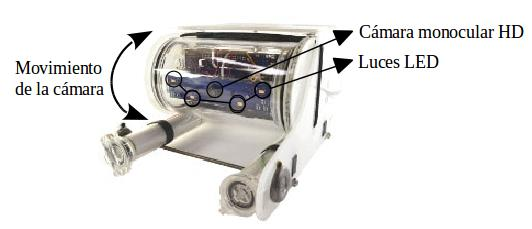
\includegraphics[width=0.7\textwidth]{openrov}
	\caption{Robot móvil OpenROV}
	\label{imagen:openrov}
\end{figure}
Si bien se cuenta con un conjunto de plataformas robóticas adaptadas para tareas de exploración, hasta el momento no se han desarrollados sistemas basados en visión que permitan incluirse en la etapa de navegación y mapeo de dichos vehículos, siendo la presente investigación la primera en abordar la tarea de la reconstrucción del suelo recorrido haciendo uso únicamente de una cámara de vídeo, sensor presente en todas las plataformas robóticas antes mencionados.

\section{Justificación y planteamiento del problema}


Cuando se habla de construir un mosaico 2D, se hace referencia al proceso de recortar y alinear imágenes, de tal forma que puedan ser representadas todas juntas en una sola gran imagen. Es importante considerar que las imágenes para este tipo de aplicaciones son capturadas desde diferentes ubicaciones de la cámara, a diferencia del proceso para elaborar imágenes panorámicas, en las cuales esta ubicación es una constante. Esta característica trae consigo uno de los principales problemas en la construcción de mosaicos, y se debe al efecto paralaje. Este efecto está asociado a la diferencia entre las posiciones aparentes de los objetos, según el punto desde donde se observa.

En la figura \ref{imagen:paralaje} se aprecia un ejemplo ilustrativo de esta definición, en la cual, si nos fijamos en el punto de vista \textbf{A}, se observa el triángulo a la izquierda del circulo, mientras que desde le punto \textbf{B} este orden se encuentra invertido. 

\begin{figure}[H]
	\centering
	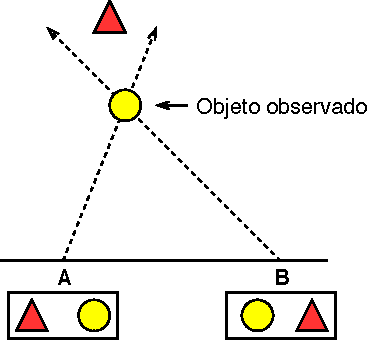
\includegraphics[width=6.5cm]{paralaje}
	\caption[Efectos en el cambio del punto de vista]{Efectos en el cambio del punto de vista.}
	\label{imagen:paralaje}
\end{figure}

Si bien, este problema afecta en gran medida la construcción del mosaico, no es el único presente, y se intensifican en aplicaciones de mapeo submarino, en las cuales, se evidencian efectos de distorsión de los objetos, absorción y cambios en la dirección de la luz, producto de pequeñas partículas suspendidas en el agua.

\begin{wrapfigure}{r}{0.3\textwidth}
	\begin{center}
		\vspace*{-0.5in}
		
\includegraphics[width=0.3\textwidth]{hugin}
	\end{center}
	\caption{Logo del software Hugin}
\end{wrapfigure}

En el \textit{GIDM} actualmente se utilizan mecanismos manuales para la elaboración de estos mapas, en especifico, se hace uso de \textit{softwares} como Hugin\footnote{\url{hugin.sourceforge.net/}}. Este es un programa de código abierto y gratuito bajo licencia GPL\footnote{ \url{http://www.gnu.org/copyleft/gpl.html}}, el cual esta dedicado a la generación de imágenes panorámicas, incluyendo funciones para el recorte, alineación y corrección de color; además de algoritmos para la optimización de parámetros en la cámara, y corrección de distorsión. Si bien este software esta diseñado para la creación de imágenes panorámicas, permite el uso de varios tipos de proyecciones cartográficas, entre estas la rectangular, proyectando las imágenes sobre un plano recto. 

Esta practica manual, además de limitar el alcance de los sistemas embebidos para el uso en navegación automática, requiere de una inversión de tiempo importante por medio del usuario en el proceso de selección y alineación de imágenes.


Atendiendo a esta necesidad, es necesario contar con un sistema que permita realizar la reconstrucción del suelo con la menor interacción posible del ser humano. Asimismo, con el fin de poder realizar operaciones de mapeo y localización simultanea \textit{SLAM} (del ingles: Simultaneous Localization and Mapping), haciendo uso de las herramientas y robots existentes en el laboratorio, se requiere contar con un sistema basado en visión, que genere de forma automática un mapa 2D de la superficie sobre la que navega o sobrevuela el vehículo remoto, y que logre lidiar de manera efectiva ante los problemas previamente planteados.


\section{Objetivos}

\subsection{Objetivo General}

Analizar e implementar un sistema automatizado que permita la reconstrucción de un mapa en dos dimensiones, del suelo recorrido por robot, aéreo o submarino, a través de la información capturada por una cámara ubicada en su parte inferior.

\subsection{Objetivos Específicos}

\begin{itemize}
	\item Análisis comparativo de métodos vigentes en la reconstrucción de mosaicos 2D, a partir de imágenes y videos de entrada.
	\item Implementación de modulo de pre-procesamiento y corrección de entrada.
	\item Análisis comparativo de métodos de detección y descripción de puntos característicos.
	\item Implementación de módulo de alineación de imágenes mediante la detección de puntos característicos.
	\item Cuantificar el error de proyección y distorsión en los modelos 2D generados.
\end{itemize}

\section{Estructura del trabajo}

Luego de presentar el planteamiento del problema y la descripción del proyecto, la presente investigación se encuentra dividida en 5 capítulos, organizados de la siguiente manera:

En el \textit{\textbf{Capitulo 2}} se presenta una revisión del estado del arte sobre los algoritmos de generación de mosaico, en el cual se exponen los trabajos recientes y avances importantes en esta área de investigación. Al mismo tiempo, se describen los módulos principales que componen este tipo de sistemas. Luego, en base a los algoritmos y técnicas estudiadas se propone un esquema para un sistemas de generación de mosaico. Para finalizar, se presenta la librería de procesamiento de imágenes que se planteó utilizar para la implementación de los algoritmos propuestos.

El \textit{\textbf{Capitulo 3}} inicia una revisión teórica en la cual se describe el funcionamiento de los algoritmos detectores, descriptores y emparejadores de características; y posteriormente se presentan resultados de pruebas comparativas entre los mas usados para este tipo de aplicaciones. 

El módulo encargado de la alineación de imágenes en el mosaico, es descrito en el \textit{\textbf{Capitulo 4}}. Al igual que el capitulo anterior, se presenta una revisión teórica de los conceptos necesarios para su implementación. Luego, se introduce el modelo de sub mosaicos, y la implementación de un conjunto de correcciones geométricas sobre este nuevo modelo. Finalmente se muestran los resultados de los algoritmos aplicados en esta sección, seguidos de sus respectivos análisis.

En el \textit{\textbf{Capitulo 5}} se describe el modulo final del sistema, en donde se explica el funcionamiento de los algoritmos que corrigen visualmente el mosaico final. De igual forma se muestran los resultados de su implementación, seguidos de una conclusión final sobre estos.

Finalmente, en el \textit{\textbf{Capitulo 6}} se presentan las conclusiones finales, además de propuestas sobre recomendaciones y posibles implementaciones que pueden aportar mejoras y/o permitir la continuación del proyecto aquí planteado.
\chapter{Sistemas de generación de mosaico}
\label{capitulo2}
\lhead{Capítulo 2. \emph{Sistemas de generación de mosaico}}

En este capítulo se presenta una revisión teórica del estado actual de las aplicaciones e investigaciones que se han desarrollado en el área de procesamiento de imágenes, aplicado a la construcción de mosaicos, además de una reseña histórica de la evolución de dichos métodos. Debido a que la construcción de mosaicos ha sido y sigue siendo un área de investigación muy activa, existe una gran variedad de métodos y técnicas que se han empleado para este fin. En este sentido se presenta una clasificación de estos algoritmo en base al modo de abordar los módulos principales en los sistemas de generación de mosaico.

Con esto se pretende recuperar y trascender el conocimiento acumulado en esta área de estudio, además de familiarizar al lector con los conceptos básicos, necesarios para la comprensión del presente trabajo. Luego, se presenta el modelo del sistema de generación de mosaico propuesto en base a los algoritmos y técnicas que se han utilizado en las investigaciones mas recientes de esta área. Finalmente se introduce la librería de procesamiento de imágenes que se seleccionó para la implementación de todos los módulos necesarios.

\section{Estado del arte}

La elaboración de mosaicos para la construcción de mapas del suelo, se ha desarrollado incluso antes desde la era digital de la computadoras. Desde que el proceso de registrar fotografías ha existido, se comenzaron a usar para elaborar mapas topográficos \cite{primeros-mapas}, donde imágenes adquiridas a partir de globos aerostáticos o altas colinas eran unidas manualmente. Posteriormente, producto de los avances en materia de aeronáutica, el interés por la aerofotografía se incrementó en gran medida. En este mismo sentido se utilizaban aviones para el registro de imágenes a mayores altitudes, y se cubrían mayores áreas en menor cantidad de tiempo. Pero debido a que no se alcanzaban suficiente altura, y se mantenía la necesidad de registrar grandes áreas, era requerido que los mapas se construyan mediante fotografías que se superpongan, de igual forma esta tarea se llevaba a cabo mediante técnicas manuales por medio de expertos.

La necesidad de registrar áreas aun mas grandes siguió avanzando, motivado por la llegada de los satélites que eran capaces de enviar a tierra la información que obtenían de las cámaras. Los avances tecnológicos en materia de computación, y el creciente aumento de datos para esta aplicación, promovieron el desarrollo de técnicas de procesamiento digital de imágenes para dar solución a este tipo de problemas.

Con el desarrollo de cámaras cada vez mas pequeñas y portátiles, así como también la llegada de vehículos no tripulados mas compactos ---ROV, UAV, AUV--- trajeron consigo grandes avances y nuevas técnicas por parte de centros de investigación en el área de la física, robótica y visión por computadora, que buscaron aportar soluciones para la realización automática de mosaicos, con un gran enfoque en las aplicaciones mas desafiantes como los ambientes submarinos.

Tal y como se ha mencionado el proceso de generación de mosaico involucra varios pasos principales, si bien se ilustran gráficamente en la figura \ref{imagen:mosaic-process}, los podemos definir como sigue:

\begin{itemize}
	\item \textbf{Registro:} De su termino en inglés \textit{image-registration}, consiste en establecer la correspondencia geomántica entre las imágenes que componen la misma escena. Para esto, es necesario estimar la transformación geométrica que logra alinear dichas imágenes en el mismo plano.
	
	\item \textbf{Alineación:} También llamada proyección, consiste en alinear las imágenes registradas en un sistema de referencia común, es decir, con respecto a un plano re referencia. En este caso se utiliza la transformación geométrica calculada en el paso anterior.
	
	\item \textbf{Fusión:} En este paso se busca corregir los errores fotométricos o discontinuidades presentes en el mosaico luego del proceso de alineación. Estos errores aparecen, producto de errores en la estimación de las transformaciones o a cambios en la perspectiva de los objetos observados
\end{itemize}

Si bien, se han propuesto una gran cantidad de algoritmos por parte de distintos grupos de investigación en todo el mundo, esta tarea aun sigue siendo desafiante, debido mayormente a los procesos de registro y fusión de las imágenes.

Específicamente el proceso para estimar correspondencias entre las imágenes es un problema complicado, en principio debido a la naturaleza no plana de los suelos estudiados; por otro lado la reducción de discontinuidades, o inconsistencias entre imágenes consecutivas sigue siendo una tarea desafiante. De modo que la mayoría de avances e implementaciones en esta área están encaminados en resolver estos dos problemas principales, o bien mejorar los resultados de trabajos previos.

De esta forma se propone una clasificación de los algoritmos de mosaicos basada en como estos abordan los procesos de registro y fusión, además para cada clasificación se realiza una revisión teórica de cada categoría, así como también los diferentes métodos y modificaciones que han aplicado los distintos desarrolladores. 

\begin{figure}[H]
	\centerline{
		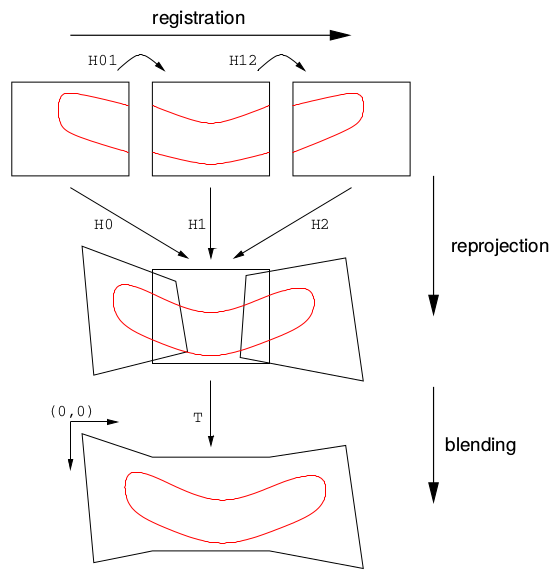
\includegraphics[width=10cm]{registration-process}}
	\caption{Proceso básico para la generación de mosaico, poner referencia, cambiar a español}
	\label{imagen:mosaic-process}
\end{figure}

\section*{Clasificación basada en el registro de imágenes}

Este proceso es muy importante para la creación de mosaicos, y básicamente es la base para estos. Cuando se registran imágenes, primero lo que se busca es encontrar la relación, o la correspondencia entre estas, teniendo en cuanta que pudieron haber sido capturadas desde distintos puntos de vista, distintos instantes de tiempo, distinta perspectiva, o incluso distintas cámaras. Luego de encontrar las zonas o puntos correspondientes, se busca estimar una matriz de transformación geométrica que permita alinearlas todas en un sistema de referencia común. Se puede decir que el registro ha sido exitoso, si se logra estimar una matriz de transformación tal que todos los puntos correspondientes se puedan unir.

Las relaciones entre las imágenes se pueden establecer utilizando distintos métodos, ya sea, emparejando puntos coincidentes, regiones enteras, o bien usando la propiedad de correlación de fase en el dominio de la frecuencia. Estos métodos para establecer correspondencias son discutidos a continuación.

\subsection*{Algoritmos en el dominio espacial}

Los algoritmos en esta categoría utilizan la información de los píxeles para establecer la relación entre imágenes, es decir, se utiliza el valor de los píxeles (intensidad) y se trata de establecer la correspondencia de estos según la ubicación en la que se encuentran. Estos se pueden separar en dos técnicas principales: basados en área o en puntos clave.

% Basados en Area

Los algoritmos basados en área, buscan relacionar dos ventanas o regiones en dos imágenes que correspondan a la misma escena. El concepto principal consiste en mover la región de interés desde la primera imagen hacia la segunda, buscando que la diferencia entre las intensidades sea la menor posible, es decir,  se trata de estimar la mejor matriz de transformación que logre reducir la diferencia de intensidades al alinear las regiones estudiadas (citar). Algunos trabajos importantes en esta clasificación utilizaron algoritmos como NCC (citar), y el MI (citar), donde estos proporcionan una métrica de igualdad entre dos imágenes. El el primer caso, el NCC mide la similitud entre las regiones estudiadas según los valores de intensidades, mientras que el MI la mide en base a la cantidad de información que comparten estas imágenes en términos de entropía. Al emplear esta técnica se logra emparejar las imágenes a nivel de píxel. Si bien se logran buenos resultados, el proceso de iterar para optimizar los parámetros de transformación y el calculo del error para cada píxel sobre las regiones, se convierte computacionalmente costoso.

% Basados en datos de Navegación



% Basados en Características

Para reducir el tiempo de computo, se utilizan algoritmos basados en la relación de características, en los cuales se tratan de detectar puntos o regiones en distintas imágenes, que correspondan con la misma ubicación. Estas características detectadas en las imágenes, se pueden evidenciar en forma de puntos aislados, curvas continuas o regiones conectadas. Luego se puede encontrar la transformación geométrica que relaciona las características de origen con las de destino, en muchos casos resolviendo una ecuación lineal. En este caso, el proceso de registro así como también el resultado del mosaico, será tan bueno como el algoritmo de detección que se utilice.

Tal y como se mencionaron los tipos de características que se pueden extraer, podemos clasificar de forma general los algoritmos de detección. Ya sea si trabajan con características locales, como lo son aquello que detectan puntos aislados. o mas globales como los basados en detección de contornos.

\subsubsection*{Detectores locales}

Al usar este tipo de algoritmos se busca encontrar la relación entre una serie de puntos dispersos que se corresponden entre dos imágenes, donde las características locales mas comunes que se suelen detectar serian esquinas, bordes, manchas, entre otros. Posteriormente el proceso de registro se completa al estimar la transformación geométrica con dicha relación de puntos, en este caso resolviendo una ecuación lineal.

Una de las ventajas principales de esta técnica para la generación de mosaicos, es que puede trabajar con imágenes consecutivas que no posean un alto nivel de cobertura. Siempre y cuando la cantidad de puntos detectados, y correctamente emparejados entre el par de imágenes supere el mínimo necesario para la solución del sistema de ecuaciones.

Diversos algoritmos detectores de características locales se han venido desarrollando desde hace mucho tiempo, y en la actualidad estos avances han permitido que el uso de este método traiga consigo muchas ventajas sobre el resto, desde variedad de aplicaciones, robustez ante distinto tipo de escenas, y velocidad de computo (siempre en función del detector a utilizar), lo que lo convierte en uno de los mas usados para la construcción de mosaicos.

\subsubsection*{Detectores globales}

Al utilizar este tipo de detectores, se busca encontrar formas, contornos, texturas, o regiones sobresalientes que se mantengan invariantes ante cambios del punto de vista o iluminación. Al igual que con los detectores locales, aquí se busca extraer tanto la posición, como el tamaño y la orientación de estas regiones.

El resto del proceso para completar la etapa de registro se mantiene igual con este método, donde la transformación geométrica se obtiene a partir de la correspondencia entre las posiciones y orientaciones de las regiones de interés que se lograron extraer. Si bien tienen buen rendimiento ante cambios de movimiento desafiantes, su uso implica un aumento en el tiempo de computo. Entre las investigaciones mas importantes dentro de esta categoría se pueden encontrar (citar).

\subsection*{Algoritmos en el dominio frecuencial}

Ya se ha visto que los algoritmos que operan en el dominio espacial cubren la mayoría de las aplicaciones e investigaciones. Sin embargo se pueden encontrar métodos que obtienen los parámetros óptimos para la transformación a partir de cálculos en el dominio de la frecuencia. 

Estos algoritmos utilizan la propiedad de correlación de fase para lograr su objetivo. Donde para un par de imágenes que se encuentran relacionadas por una simple traslación, el funcionamiento consiste en calcular la correspondiente transformada de \textit{Fourier}, luego el espectro de la potencia cruzada entre ambas. De aquí, se asegura que la fase del espectro de la potencia cruzada corresponde con la diferencia de traslación entre las dos imágenes. Finalmente el proceso continua similarmente a los métodos anteriores, alineando las imágenes según la transformación obtenida, seguido del proceso de fusionarlas.

Tal y como se explicó este proceso para una traslación, se tienen diversos trabajos como (citar) que añaden modificaciones para permitir otro tipo de transformaciones a parte de la rotación, e incluso otros que admiten cambios en la escala (citar). Si bien, los trabajos mencionados presentaron importantes, se requiere de un buen porcentaje de cobertura entre las imágenes, presenta limitaciones en los grados de libertad de las transformaciones geométricas que se pueden estimar.


\section*{Clasificación basada en el fusión de imágenes}

Si bien el proceso de registro de imágenes es fundamental para lograr un mosaico correcto, el paso final de unir las imágenes también es de gran importancia. Teniendo en cuenta que se busca aparentar que todas las imágenes componen una sola, es vital que se logre un mapa final sin inconsistencias o discontinuidades producto de los cambios en iluminación, objetos en movimiento, entre otros.

Debido a la importancia de este paso, numerosos métodos para lidiar con este tipo de problemas se han desarrollado, lo que nos permite también clasificar los algoritmos de generación de mosaico según como aborden este problema. Entre los métodos mas utilizados encontramos: fusionar las imágenes mediante cambios suavizados o buscan la mejor linea de corte entre estas.

\subsection*{Transición suavizada}

Los algoritmos de esta categoría buscan minimizar la diferencia entre dos imágenes suavizando los bordes donde se superponen. FALTA INTRO

El método mas simple para fusionar dos imágenes, consiste en realizar una suma ponderada sobre el área de superposición entre ambas, ponderando la intensidad de cada imagen a la mitad. Al realizar esta operación se suelen tener efectos indeseados como el efecto fantasma, donde se pueden observar duplicados del mismo objeto con cierto nivel de desvanecimiento. Esto de sebe a errores en el proceso de alineación de las imágenes, diferencia en la iluminación, o incluso a objetos móviles. 

Para evitar esto, se utiliza un proceso de fusión que consiste en realizar una suma ponderada entre ambas imágenes, pero dando mayor ponderación a las regiones que se encuentren mas cerca del centro de la imagen, y menor a aquellas que se encuentren cerca el borde. Si bien, se logra reducir posibles discontinuidades entre los bordes originales, el efecto fantasma aun se puede apreciar para imágenes con fuertes problemas de alineación.

Considerando este problema, y con el objetivo de realizar una unión mas robusta, se desarrolló un esquema piramidal de fusión ponderada. El proceso consiste en obtener una imagen laplaciana para distintos tamaños de escala formando así una pirámide, al mismo tiempo se va creando para cada escala una mascara, la cual será la mascara original difuminada por el efecto del filtro gaussiano. Luego para cada nivel de la pirámide se aplica el algoritmo de fusión ponderada descrito previamente donde la mascara  difuminada pondera el valor de cada píxel. Entre los trabajos que aplican este algoritmo obteniendo resultados notables se tienen (citar), logrando reducir en gran medida el efecto duplicado en las regiones de superposición.

\subsection*{Linea de corte óptima}

En lugar de buscar reducir las posibles discontinuidades a partir de una suave transición a través del borde entre dos imágenes, en este tipo de algoritmo se busca modificar este borde. Es decir, se trata de encontrar la linea de corte en el área de superposición que logre reducir la discontinuidad de texturas entre ambas imágenes. La diferencia principal de este método sobre los anteriores, es que se toma en cuenta la información presente en la región que se desea fusionar, permitiendo que se logre remover errores producidos por el efecto paralaje, o debido a objetos móviles dentro de la escena. Por otra parte, como las regiones resultantes luego de la linea de corte no se comparten información, se pueden presentar discontinuidades producto de grandes diferencias de iluminación.


\section{Esquema propuesto}

\begin{figure}[H]
	\centerline{
		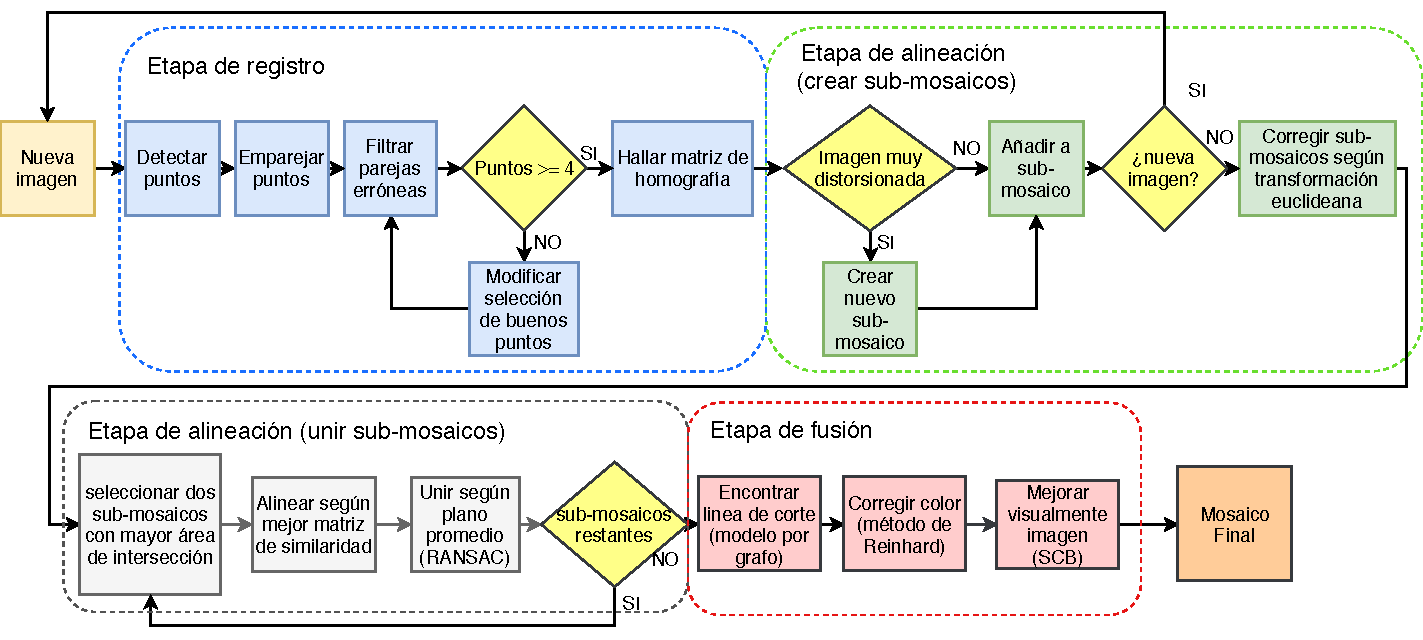
\includegraphics[width=1.21\textwidth]{esquema-general}}
		\caption{Esquema propuesto para la construcción del mosaico}
	
	\label{imagen:esquema}
\end{figure}

\section{Librería de desarrollo}

\subsection{OpenCV}
\chapter{Detección de puntos de interés}
\label{capitulo3}
\lhead{Capítulo 3. \emph{Detección de puntos de interés}}


\section{Introducción}


\section{Revisión teórica}

\subsection{Detectores y descriptores de características}

Antes mencionar la evolución de los algoritmos de detección de puntos de interés, primero es necesario definir que son estos. Los puntos de interés, puntos clave, o \textit{"features"} (en español: características) como son comúnmente llamados, son regiones en una imagen que contienen patrones específicos, lo que hace que puedan ser fácilmente seguidos o ubicados en otra imagen. Tuytelaars y Mikolajczyk \cite{Tuytelaars} definen un punto característico local como \textit{``un patrón en la imagen que difiere de su vecindario directo''}. De esta forma, se considera que los puntos característicos deben proporcionar la posibilidad de ser identificados en diferentes imágenes con el objetivo de emparejarlos.

Para alcanzar este objetivo los detectores y extractores de puntos característicos deben cumplir con ciertas propiedades que les permita funcionar bajo distintas condiciones, en concreto se busca que estos algoritmos cumplan con las siguientes propiedades:

\begin{itemize}
	\item \textbf{Robustez:} El algoritmo debe ser capaz de detectar la misma ubicación del punto característico independientemente ante cambios en la escala, rotación, traslación, iluminación, transformaciones geométricas, artefactos de compresión y ruido.
	
	\item \textbf{Repetibilidad:} El algoritmo debe ser capaz de detectar el mismo punto característico de la misma escena bajo cambios en el punto de vista.
	
	\item \textbf{Exactitud:} El detector debe localizar el punto característico de manera precisa (misma ubicación de pixel). Especialmente para tareas de alineación de imágenes.
	
	\item \textbf{Generalidad:} El algoritmo debe ser capaz de detectar puntos que pueden ser usadas en distintas aplicaciones, es decir, que detecte varios tipos de características (esquinas, burbujas, etc.)
	
	\item \textbf{Eficiencia:} El algoritmo debe ser capaz de detectar puntos característicos en nuevas imágenes a gran velocidad, para soportar aplicaciones en tiempo real.
	
	\item \textbf{Cantidad:} El algoritmo debe detectar todos, o casi todos los puntos característicos presentes en la imagen. 
	
\end{itemize}



\begin{figure}[H]
	\centering
	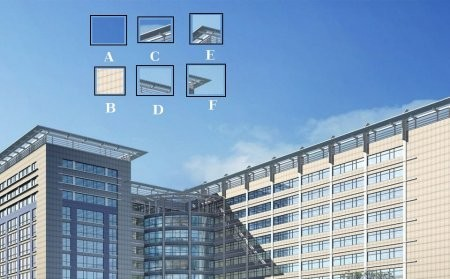
\includegraphics[width=0.7\textwidth]{features}
	\caption{Caracterización de regiones en una imagen}
	\label{imagen:features}
\end{figure}

Llegados a este punto es necesario definir el funcionamiento de los algoritmos detectores, y que consideran estos como puntos característicos, basados en la definición previamente planteada. Atendiendo a la imagen \ref{imagen:features}, se puede observar que se caracterizan seis áreas de interés. Analizando estos segmentos, vemos que \textbf{\textit{A}} y \textbf{\textit{B}} corresponden con superficies planas, lo que hace que sea muy difícil identificar la ubicación exacta de estas superficies en la imagen original. Por otro lado, tenemos las regiones \textbf{\textit{C}} y \textbf{\textit{D}}, las cuales corresponden con bordes en la imagen, si bien, se puede limitar en gran medida el área de búsqueda hacia toda las regiones del mismo bordes, sigue siendo difícil acertar con la ubicación correcta. Por ultimo, analizando las regiones \textbf{\textit{E}} y \textbf{\textit{F}} tenemos que corresponden a esquinas de la imagen original, en este caso se puede identificar fácilmente la ubicación exacta de la región en la imagen.

A partir de esta idea, en la cual se consideran las esquinas como regiones fácilmente identificables en una imagen, en \textit{1988} nace el primer algoritmo de detección de puntos de interés llamado Detector de esquinas de Harris \cite{harris} (nombre original en inglés: Harris Corner Detector), y como su nombre lo indica está basado en la detección de esquinas.

Retomando el concepto planteado previamente, este detector busca la diferencia de intensidad de una región con su entorno directo, es decir, se detectará una esquina para aquellas regiones que presenten una alta variación de intensidad, al desplazar la ventana estudiada en cualquier dirección. En la figura \ref{imagen:harris-window} se puede apreciar visualmente como funciona esta ventana de búsqueda.

\begin{figure}[H]
	\centering
	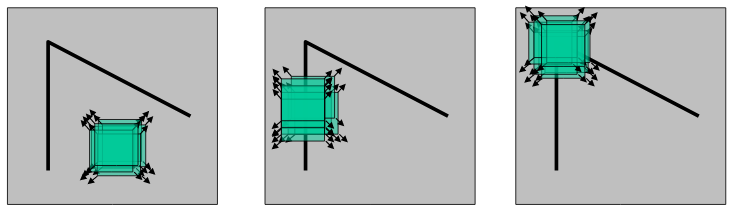
\includegraphics[width=0.9\textwidth]{harris-window}
	\caption{Ventana de búsqueda para de detección de esquinas}
	\label{imagen:harris-window}
\end{figure}

Cuando se trabajan con detectores de características, se desea que estos sean invariantes ante la mayor cantidad de variables posibles, tal y como se menciona en la propiedad de robustez que deben tener estos algoritmos. Si bien el detector presentado anteriormente es invariante ante la traslación y la rotación (ya que las esquinas se mantienen como esquinas si son rotadas o desplazadas), no funciona de la misma forma ante cambios de escala. Como se observa en la figura \ref{imagen:corner-scale}, una región considerada como esquina, se podría considerar plana si es ampliada.

\begin{figure}[H]
	\centering
	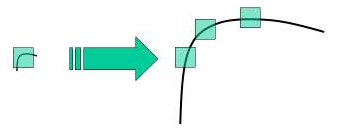
\includegraphics[width=0.85\textwidth]{corner-scale}
	\caption{Efecto del escalado sobre las esquinas}
	\label{imagen:corner-scale}
\end{figure}

Con el fin de conseguir detectar los mismos puntos ante cambios en la escala de la imagen, Lindeberg, T. \cite{log} propone un algoritmo detector de ``manchas'' multi-escala a través de la búsqueda de un máximos en el espacio de escala, el cual se crea utilizando un operador laplaciano. El Laplaciano de Gaussianas \textit{LoG} (del ingles: Laplacian-of-Gaussian), es una combinación lineal de segundas derivadas utilizado para detectar burbujas o manchas en una imagen. El funcionamiento es el siguiente: Dada una imagen de entrada, la representación para cada escala $-s-$ de la imagen se define como la convolución de la imagen con un filtro Gaussiano con desviación estándar $s$.

Este resultado brinda una fuerte respuesta positiva para burbujas oscuras y respuestas fuertes negativas para burbujas claras, ambas de un tamaño 2$s$, donde $s$ es la escala. De esta forma las caracteristicas detectadas presentan una fuerte relación entre el tamaño de las estructuras en la imagen y el grado de difusión del filtro gaussiano. Donde la desviación estándar del filtro se usa para controlar la escala cambiando que tanto se difumina la imagen.

Llegados aquí, una vez se haya detectado la ubicación de los puntos característicos en la imagen, la información de la localidad de este debe ser codificada y almacenada, y de esta forma lograr tener un descriptor único de la región con el objetivo final de ubicarlo en otra imagen. Con este fin se desarrollaron los algoritmos descriptores, los cuales una vez tengan la ubicación de los puntos característicos se encargan de convertir la información de su alrededor en una serie de números, o un vector que permita diferenciar un punto clave de otro. Esta información también es necesaria que sea invariante ante las variable mencionadas previamente, para lograr una identificación eficiente del mismo punto en distintas imágenes bajo distintas condiciones.

Partiendo de estos problemas, y del hecho que el calculo del operador LoG es computacionalmente costoso, en \textit{2004 D. Lowe} crea el detector y descriptor \textit{SIFT} \cite{sift} (del inglés: Scale Invariant Feature Transform), en el cual el espacio de escala es construido en forma piramidal con la diferencia de gaussianas DoG (del inglés: Difference of Gaussians). En este sentido, El operador DoG ofrece una aproximación al LoG, donde se calcula sin convolución restando niveles de escala adyacentes de una pirámide gaussiana. El proceso para la detección y descripción de puntos de interés de este algoritmo, consta de cuatro pasos principales:

En primer lugar, realiza una detección de máximos en el espacio de la escala aplicando la diferencia gaussiana \textit{DoG}. Para esto, se aplica el filtro gaussiano con distintos tamaños de media (se tienen distintas escalas), luego restando estas imágenes para distintos pares de escalas se logra la diferencia de gaussiana. Posteriormente se buscan los máximos locales a lo largo del espacio (coordenadas X,Y) para cada correspondiente escala. Este proceso de detección se puede visualizar en la figura \ref{imagen:sift-escalas}.

\begin{figure}[H]
	\centering
	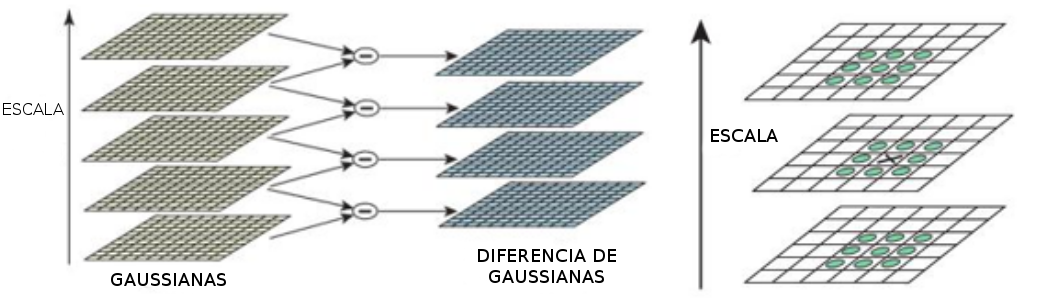
\includegraphics[width=0.85\textwidth]{sift-escalas}
	\caption{Detección de máximos en el espacio de la escala DoG}
	\label{imagen:sift-escalas}
\end{figure}

En segundo lugar para la localización de puntos de interés, se descartan los puntos encontrados en el paso anterior que no superen cierto valor de umbral, es decir, que no estén lo suficientemente contrastados con su entorno. Con esta etapa el algoritmo solo toma en cuenta los puntos claves mas fuertes por cada escala. Además, con el objetivo de eliminar los bordes suficientemente contrastados que no correspondan con esquinas, el algoritmo usa una matriz hessiana para calcular las curvaturas principales, y así quedarse solo con esquinas.

Para garantizar la invarianza con respecto a la rotación, se toman los píxeles vecinos al punto clave y se calcula la magnitud y dirección del gradiente en esa región. Con esto se hace un histograma de la magnitud del gradiente en cada dirección, donde el pico mayor del histograma indica la orientación. En el caso que exista un pico mayor al 80\% del pico principal, este se utiliza para crear otro punto de interés en la misma posición pero con la distinta rotación.

Finalmente para crear el vector descriptor por cada punto clave se crea una matriz de 16x16 alrededor de este, dividida en 4 subregiones de 4x4 píxeles con un histograma de orientaciones para cada uno. Seguidamente, el descriptor del punto será el vector con los valores de los histogramas de las regiones 4x4 concatenados. La figura \ref{imagen:descriptor} la representación del descriptor de SIFT.

\begin{figure}[H]
	\centering
	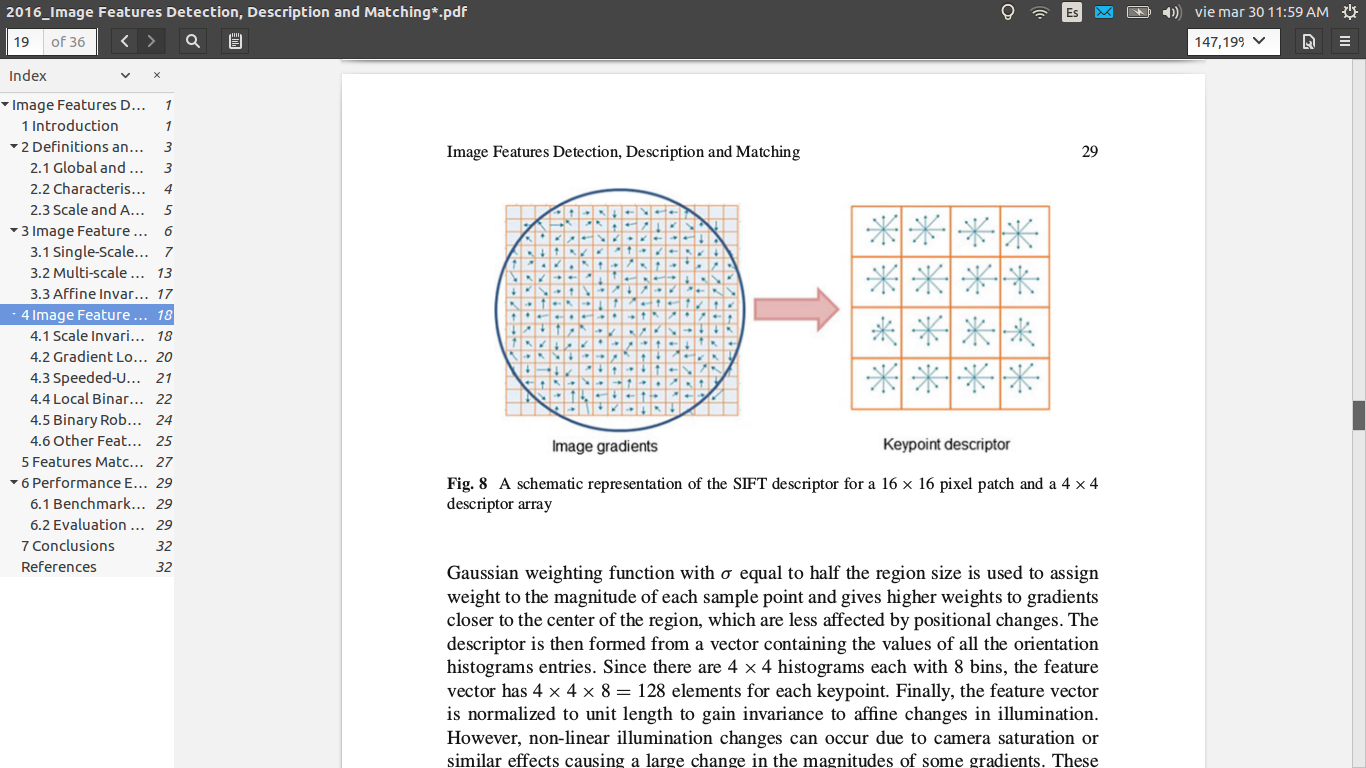
\includegraphics[width=0.7\textwidth]{sift-descriptor}
	\caption{Descriptor del algoritmo SIFT}
	\label{imagen:descriptor}
\end{figure}


En el año 2006, un grupo de tres  personas Bay, H., Tuytelaars, T. and Van Gool, L. desarrollan \textit{SURF} \cite{surf}, el cual es un detector y descriptor de características basado en SIFT, pero con modificacioes que aumentan su velocidad de detección. Si bien, sacrifica un poco de rendimiento y precisión, lo hace mas provechoso para aplicaciones embebidas que demanden mayor velocidad de computo y menor uso de recursos, como por ejemplo \textit{SLAM}. El proceso para la extracción de características por parte de este algoritmo se compone de los siguientes pasos:

Como primer paso, en lugar de aproximar el laplaciano de Gauss \textit{LoG} (del inglés: Laplacian of Gaussians) con la diferencia de Gaussianas (DoG) como lo hace SIFT, este algoritmo aproxima LoG con cuadrados para promediar la imagen. La ventaja de aplicar filtros con cuadrados es que con la ayuda de imágenes integrales el cálculo computacional se reduce en gran medida.

\begin{figure}[H]
	\centering
	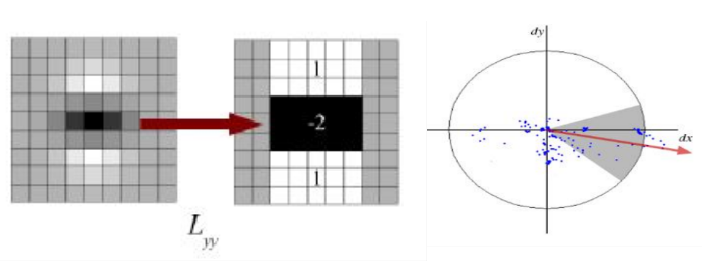
\includegraphics[width=0.8\textwidth]{surf}
	\caption{Deteccion y descripción mediante el algoritmo SURF}
	\label{imagen:surf}
\end{figure}

En función de identificar la orientación, el algoritmo utiliza la respuesta wavelet Haar en horizontal y vertical en un vecindario de 6$s$ (donde $s$ es la escala evaluada) píxeles al rededor del punto de interés, Luego estas respuestas son representadas como puntos en el espacio, para luego calcular la orientación dominante con la suma de todos los resultados dentro de una ventana deslizante de apertura 60$^\circ$. En la figura \ref{imagen:surf} se puede visualizar en el lado izquierdo, la aproximación que realiza de la derivada de segundo orden del filtro gaussiano, y su aproximación con un filtro cuadrado. Del lado derecho se ilustra el vector de orientación en función a la distribución de puntos estudiados.

El siguiente avance importante en los algoritmos de detección aparece en el año 2011 con \textit{ORB} \cite{orb} (del inglés: Oriented FAST and Rotated BRIEF), este utiliza una combinación del detector FAST (del inglés: Features from Accelerated Segment Test) y del descriptor BRIEF (del inglés: Binary Robust Independent Elementary Features), este nuevo algoritmo esta caracterizado por su alta velocidad de procesamiento manteniendo un buen rendimiento, gracias al uso de un descriptor binario. 

Como se mencionó utiliza el algoritmo FAST, el cual consiste en encontrar esquinas evaluando los píxeles en un perímetro circular, de esta forma, un punto será detectado como esquina si la cantidad de píxeles de color opuesto al evaluado, supera cierto valor de umbral (ver izquierda en la figura \ref{imagen:orb}), posteriormente con el fin de aumentar la robustez, es aplicado el algoritmo de clasificación de esquinas de $Harris$. De igual forma se realiza con una estructura piramidal evaluando varias escalas (al igual que SIFT).

\begin{figure}[H]
	\centering
	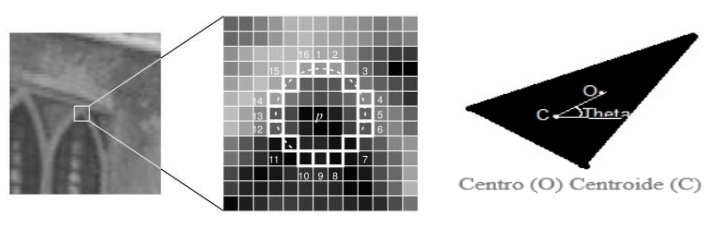
\includegraphics[width=0.9\textwidth]{orb}
	\caption{Deteccion y descripción mediante el algoritmo SURF}
	\label{imagen:orb}
\end{figure}

Como el algoritmo FAST no toma en cuenta la orientación, en el ORB se modificó para que calculara la orientación de la siguiente forma: Se considera una región ubicada en el centro del punto estudiado, luego se calcula el centroide de la región en función a la intensidad de los puntos. De esta forma, la dirección del vector desde el punto central  hasta el centroide es asignado como vector de orientación. Observando a la derecha en \ref{imagen:orb} se aprecia un ejemplo del lugar del centroide \textit{(C)} y del centro \textit{(O)} par auna región en particular.


Para el descriptor utiliza BRIEF, a diferencia de los anteriores (SIFT y SURF) este es un descriptor binario y no vectorial. El descriptor BFIEF produce una palabra de $n$-bits usando el algoritmo \textit{Local Binay Tests} (LBT), el problema de esta representación es que no es muy robusta ante cambios en la rotación. Para resolver esto ORB utiliza la información de la orientación previamente calculada en el paso de detección para aplicar LBT en esa orientación.

Los algoritmos de detección que se mencionaron hasta este momento tienen una caracteristica en común, y es que cuando trabajan con el esquema piramidal lo hacen bajo el espacio de escala Gaussiano, el cual es una instancia particular de difusion lineal. De esta forma, al utilizar este filtro no se respetan los limites naturales de los objetos y se difumina del mismo nivel toda la region de la imagen cuando se avanza entre nieveles de escala.

Enfocándose en esta característica, en el año de \textit{2012} se desarrolla el detector y descriptor llamado KAZE \cite{kaze} por parte de \textit{Pablo Fernández Alcantarilla}. Este novedoso algoritmo opera completamente en un espacio de escala no lineal, y para ello utilizan un esquema de división de operadores aditivos (\textit{AOS}, del inglés: Additive Operator Splitting), que les permite obtener espacios de escala no lineales de forma eficiente. De este modo se puede realizar un difuminado localmente adaptativo, posibilitando que se remueva el ruido en las imágenes, manteniendo información importante sobre los bordes de los objetos al avanzar en el espacio de escala. En la figura \ref{imagen:kaze} se puede observar como afecta en los bordes de los objetos el aplicar un filtro de difusión lineal, y uno que no lo es, bajo el esquema propuesto por este algoritmo.

\begin{figure}[H]
	\centering
	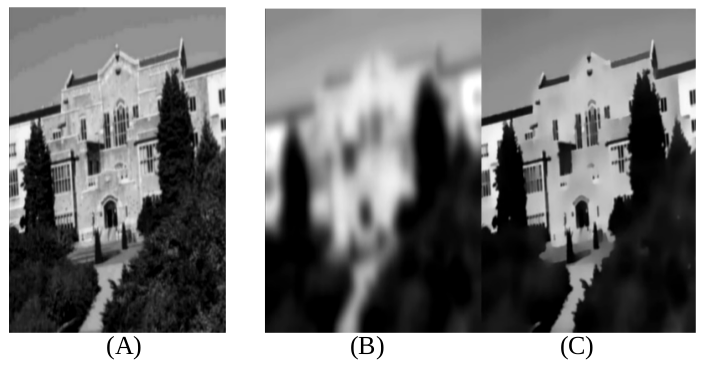
\includegraphics[width=0.85\textwidth]{kaze}
	\caption[Filtro no lineal propuesto por KAZE]{\textit{(A)}: imagen original, \textit{(B)} filtro lineal Gaussiano, \textit{(C)} filtro no lineal usado en KAZE}
	\label{imagen:kaze}
\end{figure}

Bajo este mismo esquema de difusión no lineal, el mismo autor en el año \textit{2013} desarrolla la versión acelerada de este algoritmo que recibe el nombre de \textit{A-KAZE} \cite{akaze} (del ingles: Accelerated KAZE). Esta mejora se utiliza un esquema basado en difusión explícita rápida \textit{FED} (del ingles: Fast Explicit Difussion) en lugar de \textit{AOS}, el cual es un nuevo esquema piramidal que incrementa en gran medida la velocidad de computo para construir el espacio de escala no lineal.

Para el calculo de la orientación el primer algoritmo \textit{KAZE} utiliza un descriptor para la orientación similar al que emplea SURF. Este encuentra la orientación dominante en un área circular de radio 6$s$ ($s$ corresponde con la escala), y para cada muestra del círculo se calcula la derivada de primer orden en las direcciones $X$ e $Y$, y se ponderan con una gaussiana centrada en el punto de interés. Luego, las respuestas de estas derivadas son representadas como puntos en un espacio vectorial, donde la orientación dominante se haya sumando las respuestas dentro de un segmento de circulo deslizante con apertura de 60$^\circ$.

Por otro lado, la versión acelerada \textit{A-KAZE} emplea un descriptor basado en una versión modificada del algoritmo de diferencia local binaria \textit{LDB} \cite{ldb} (del ingles: Local Difference Binary), llamado M-LBD (del ingles: Modified Local Difference Binary), el cual aprovecha al máximo la información del espacio de escala no lineal. La modificación consiste en hacer un sub-muestreo de cada región que divide la zona del descriptor, en lugar de calcular el promedio de todos los píxeles de la región, es decir, se tienen muestras de cada subdivisión para distintas escalas.


\subsection{Emparejadores de puntos característicos}

Emparejadores

\section{Implementación y resultados de modulo comparativo}

\section{Conclusiones}

Resumen
\chapter{Alineación de imágenes}
\label{capitulo4}
\lhead{Capítulo 4. \emph{Alineación de imágenes}}

\section{Introducción}

De la sección anterior estudiamos la primera etapa del proceso de registro de imágenes, estableciendo la correspondencia de puntos entre estas. Ahora bien, en esta sección se continúa la etapa de registro pero abordando el tema de las transformaciones geométricas, en primer lugar presentando una descripción y explicación de su estructura y seguido del proceso de su estimación a partir de los puntos previamente obtenidos. Una vez la etapa de registro este completa, se profundiza en el proceso para la alineación de imágenes en un plano común, presentando los algoritmos utilizados para su implementación, así como también técnicas para reducir el error acumulado de las etapas anteriores. Finalmente se presentas resultados por separado de cada proceso previamente descrito, con su respectivo análisis.

\section{Revisión teórica}

A continuación se expone una revisión de los conceptos básicos que involucran una transformación geométrica, donde se plantea una jerarquía de los distintos niveles de transformaciones basadas en sus propiedades geométricas. Una vez se tengan claros estos conceptos, se presentan los métodos matemáticos que permiten obtener dichas transformaciones. 

\subsection{Transformaciones geométricas}

El siguiente paso en el proceso de registro, luego de establecer la correspondencia entre las imágenes, es encontrar la transformación geométrica que permite alinearlas. Para comprender su funcionamiento primero es necesario introducir el concepto de espacio proyectivo, sobre el cual se efectuarán dichas transformaciones. En base a esto comenzaremos presentando la notación homogénea para puntos y lineas en este espacio.

Una linea en el espacio representada por la ecuación $ax + by + c = 0$, se puede expresar en forma vectorial de la forma $(a,\, b,\, c)$. Así, los vectores $k(a,\, b,\, c)$ representan todo el conjunto de rectas que son equivalentes --- $(ka)x + (kb)y + (k)c = 0$ ---, para cualquier $k\neq0$. De esta forma, se conoce como un vector homogéneo al vector particular que pertenezca a un grupo de vectores bajo esta relación de equivalencia. En base a este concepto se introduce la definición \ref{espacio-p} de espacio proyectivo.

\begin{displayquote}
	\vspace{-1.5cm}
	\begin{definition}
		El espacio proyectivo ${\rm I\!P}^2$ está conformado por el grupo de rectas o vectores equivalentes en el conjunto ${\rm I\!R}^2-\{0\}$, es decir, excluyendo la recta $(0,\, 0,\, 0)$.
		\label{espacio-p}
	\end{definition}
\end{displayquote}

Conociendo el espacio proyectivo, y la notación de vectores homogéneos, es importante introducir el concepto de puntos homogéneos, y establecer una relación que nos permita transformarlos a su espacio euclidiano original. 

Teniendo un punto $\vec{x}=(x,\, y)$, este pertenece a la recta $\vec{l}=(a,\, b,\, c)$ si logra satisfacer su ecuación --- $ax + by + c = 0$ ---. Si lo escribimos en forma vectorial, tendríamos $(x,\, y,\, 1)(a,\, b,\, c) = 0$, esto es añadiendo un 1 como tercer componente del punto $\vec{x}$. Similar al concepto previo de vectores homogéneos, se tiene que el conjunto de puntos $k(x,\, y,\, 1)$ son representaciones equivalentes del mismo punto, ya que todo ese conjunto pertenece a la misma recta --- $k(x,\, y,\, 1)(a,\, b,\, c) = 0 \to (ka)x + (kb)y + (k)c = 0$ ---. Así, añadiendo esta coordenada, tenemos que los puntos son representados como vectores homogéneos y pertenecen al espacio ${\rm I\!P}^2$. De esta forma se introduce la siguiente definición \ref{punto-homogeneo} que relaciona la siguiente conversión: ${\rm I\!P}^2 \to {\rm I\!R}^2$.
\begin{displayquote}
	\vspace{-1.5cm}
	\begin{definition}
		La representación de un vector homogéneo es de la forma $\vec{x} = (x_1,\, x_2,\, x_3)$, representando el punto $(x_1/x_3,\, x_2/x_3)$ en ${\rm I\!R}^2$, con $x_3 \neq 0$.
	\end{definition} 
	\label{punto-homogeneo}
\end{displayquote}

Teniendo claros los conceptos de representación homogénea, se presenta formalmente la definición de una homografía (\ref{def-homografia}) o transformación geométrica en el espacio proyectivo.
\begin{displayquote}
	\vspace{-1.5cm}
	\begin{theorem}
		Una transformación $h : {\rm I\!P}^2 \to {\rm I\!P}^2$ es una homografia si y solo si existe una matriz no singular $\vec{H}_{3x3}$, para la cual, cualquier punto en ${\rm I\!P}^2$ representado por un vector $\vec{x}$ se cumple que $h(\vec{x}) = \vec{H}\,\vec{x}$.
		\label{def-homografia}
	\end{theorem} 
\end{displayquote}

Existen varias formas de describir las transformaciones geométricas, la primera es algebraica, en la cual se muestra la estructura de la matriz de transformación, y la segunda es analizando las variables que se preservan, o que se mantienen invariantes luego de aplicar dicha transformación. Adicionalmente, cada transformación geométrica está caracterizada por los grados de libertad, o la cantidad de parámetros que cada una puede variar sobre la imagen de entrada. Esta definición se introduce a continuación (\ref{def-dof}).
\begin{displayquote}
	\vspace{-1.5cm}
	\begin{definition}
		Los grados de libertad \textit{DoF} (del inglés: Degrees of Freedom), son la cantidad mínima de parámetros independientes que pueden especificar el movimiento de un objeto. En otras palabras, es la mínima cantidad de movimientos independientes que puede realizar un objeto. En el caso de transformaciones geométricas, corresponde con el numero de componentes "libres" que permiten especificar dicha transformación.
		\label{def-dof}
	\end{definition} 
\end{displayquote}

En base a los grados de libertad, a las propiedades geométricas y al tipo de invarianza que presenten, se tienen cuatro niveles de transformaciones geométricas: isometría, similaridad, afín y perspectiva. Estos son descritos a continuación.
%${\rm I\!P}^2$, ${\rm I\!R}$ 
%%%%%%%%%%%%%%%%%%%%%%%%%%%%%%%%%%%%%%%%%%%%%%%%%%%%%%%%%%
\subsubsection*{ISOMETRÍA}

Este termino proviene del griego iso (igual) metria (medida), y tal como su nombre lo indica, ésta transformación se caracteriza fuertemente por mantener iguales las longitudes entre todos los puntos. Ésta se compone por una combinación de rotaciones y translaciones --- transformaciones euclidianas --- donde se modela el movimiento de un objeto rígido. En la ecuación \ref{matriz-isometria} se puede observar su representación matricial.

\begin{equation}
	\begin{pmatrix}
	{x'}\\{y'}\\{1}
	\end{pmatrix} = 
	\begin{bmatrix}
	{\cos \theta}&{-\sin \theta}&{tx}\\
	{\sin \theta}&{\cos \theta}&{ty}\\
	{0}&{0}&{1}
	\end{bmatrix}
	\begin{pmatrix}
	{x}\\{y}\\{1}
	\end{pmatrix}
	\label{matriz-isometria}
\end{equation}
\begin{displaymath}
(x', \,y', \,1) \to (x',\, y') 
\end{displaymath}
Esta matriz es posible expresarla por bloques, como se muestra a continuación:
\begin{displaymath}
\vec{x'}= 
\begin{bmatrix}
{\mathtt{R}}&{\vec{t}}\\
{\vec{0}}&{1}
\end{bmatrix}
\vec{x}
\label{bloque-isometria}
\end{displaymath}
Donde $ \mathtt{R} $ sería una matriz ortogonal de rotación $2\times2$, $ \vec{t} $ es un vector columna de translación de 2 componentes y $\vec{0} $ es un vector fila nulo de 2 componentes.
\begin{itemize}
	\item \textbf{Invarianza:} Distancia entre puntos, ángulo entre lineas y área.
	\item \textbf{3 Grados de libertad:} Ángulo de rotación, traslación en eje $x$, traslación en eje $y$. Puede ser calculada a partir de dos puntos correspondientes.
\end{itemize}

%%%%%%%%%%%%%%%%%%%%%%%%%%%%%%%%%%%%%%%%%%%%%%%%%%%%%%%%%%
\subsubsection*{SIMILARIDAD}

Esta transformación es una combinación de una isometría con un escalado, en este caso el escalado es de igual magnitud en los ejes $x$ e $y$. La representación matricial se observa en la ecuación \ref{matriz-similaridad}.

\begin{equation}
\begin{pmatrix}
{x'}\\{y'}\\{1}
\end{pmatrix} = 
\begin{bmatrix}
{s\, \cos \theta}&{-s\, \sin \theta}&{tx}\\
{s\, \sin \theta}&{s\, \cos \theta}&{ty}\\
{0}&{0}&{1}
\end{bmatrix}
\begin{pmatrix}
{x}\\{y}\\{1}
\end{pmatrix}
\label{matriz-similaridad}
\end{equation}
\begin{displaymath}
(x', \,y', \,1) \to (x',\, y')
\end{displaymath}
Esta matriz es posible expresarla por bloques, como se muestra a continuación:
\begin{displaymath}
\vec{x'}= 
\begin{bmatrix}
{s\mathtt{R}}&{\vec{t}}\\
{\vec{0}}&{1}
\end{bmatrix}
\vec{x}
\label{bloque-similaridad}
\end{displaymath}
Donde $ \mathtt{R} $ sería una matriz ortogonal de rotación $2\times2$, $s$ es el factor de la escala, $ \vec{t} $ es un vector columna de translación de 2 componentes y $\vec{0} $ es un vector fila nulo de 2 componentes.

\begin{itemize}
	\item \textbf{Invarianza:} Cociente de longitudes, Ángulo entre lineas y área.
	\item \textbf{4 Grados de libertad:} Ángulo de rotación, traslación en eje $x$, traslación en eje $y$. Puede ser calculada a partir de dos puntos correspondientes.
\end{itemize}

%%%%%%%%%%%%%%%%%%%%%%%%%%%%%%%%%%%%%%%%%%%%%%%%%%%%%%%%%%
\subsubsection*{AFÍN}

La transformación afín (también llamada afinidad) está compuesta por una transformación lineal (rotación, sesgo, homotecia), seguida de una translación. En está se tiene una transformación mas compleja que las anteriores, ya que se incluyen algunas deformaciones que no permiten conservar la forma original de los objetos. De igual forma puede incluirse un escalado, pero a diferencia de la anterior, éste puede ser de distinta magnitud en los ejes $x$ e $y$. La representación matricial se observa en la ecuación \ref{matriz-afin}.

\begin{equation}
\begin{pmatrix}
{x'}\\{y'}\\{1}
\end{pmatrix} = 
\begin{bmatrix}
{a_{11}}&{a_{12}}&{tx}\\
{a_{2s1}}&{a_{22}}&{ty}\\
{0}&{0}&{1}
\end{bmatrix}
\begin{pmatrix}
{x}\\{y}\\{1}
\end{pmatrix}
\label{matriz-afin}
\end{equation}
\begin{displaymath}
(x', \,y', \,1) \to (x',\, y')
\end{displaymath}
Esta matriz es posible expresarla por bloques, como se muestra a continuación:
\begin{displaymath}
\vec{x'}= 
\begin{bmatrix}
{\mathtt{A}}&{\vec{t}}\\
{\vec{0}}&{1}
\end{bmatrix}
\vec{x}
\label{bloque-afin}
\end{displaymath}
Donde $ \mathtt{A} $ sería una matriz ortogonal $2\times2$ no singular, $\vec{t} $ es un vector columna de translación de 2 componentes y $\vec{0} $ es un vector fila nulo de 2 componentes.

\begin{itemize}
	\item \textbf{Invarianza:} Lineas paralelas, cociente de longitudes de lineas paralelas.
	\item \textbf{6 Grados de libertad:} 4 componentes de la matriz lineal, traslación en eje $x$, traslación en eje $y$. Puede ser calculada a partir de tres puntos correspondientes.
\end{itemize}

%%%%%%%%%%%%%%%%%%%%%%%%%%%%%%%%%%%%%%%%%%%%%%%%%%%%%%%%%%
\subsubsection*{PROYECTIVA}

Por último se presenta la transformación proyectiva u homografía. Las transformaciones mostradas anteriormente  tienen en común la ultima fila de la matriz que la describe --- $(0,\, 0,\, 1)$ ---, lo cual hace que el tercer componente de la representación homogénea nunca cambie de 1. Por esta razón se dice que estas transformaciones son de coordenadas no-homogéneas. El caso de la homografía es distinto, ya que se tiene una transformación lineal de coordenadas homogéneas (definición \ref{punto-homogeneo}). La representación matricial se puede ver en la ecuación \ref{matriz-perspectiva}.

\begin{equation}
\begin{pmatrix}
{x'}\\{y'}\\{w}
\end{pmatrix} = 
\begin{bmatrix}
{h_{11}}&{h_{12}}&{h_{13}}\\
{h_{21}}&{h_{22}}&{h_{23}}\\
{h_{31}}&{h_{32}}&{h_{33}}
\end{bmatrix}
\begin{pmatrix}
{x}\\{y}\\{1}
\end{pmatrix}
\label{matriz-perspectiva}
\end{equation}
\begin{displaymath}
	(x', \,y', \,w) \to (x'/w,\, y'/w),\, w \neq 0
\end{displaymath}
Esta matriz es posible expresarla por bloques, como se muestra a continuación:
\begin{displaymath}
\vec{x'}= 
\begin{bmatrix}
{\mathtt{A}}&{\vec{t}}\\
{\vec{v}}&{u}
\end{bmatrix}
\vec{x}
\label{bloque-perspectiva}
\end{displaymath}
Donde $ \mathtt{A} $ sería una matriz ortogonal $2\times2$ no singular, $\vec{v}$ es un vector fila de 2 componentes, $\vec{t}$ es un vector columna de translación de 2 componentes, $\vec{0} $ es un vector fila nulo de 2 componentes y $u$ es el factor de escala de la transformación.

\begin{itemize}
	\item \textbf{Invarianza:} cociente cruzado (cociente de cocientes de longitudes), puntos de contacto (intersecciones).
	\item \textbf{8 Grados de libertad:} Si bien la matriz cuenta con 9 componentes, al escalar todos los componentes por $u$, la transformación quedaría especificada por los 8 valores restantes.
\end{itemize}
%%%%%%%%%%%%%%%%%%%%%%%%%%%%%%%%%%%%%%%%%%%%%%%%%%%%%%%%%%
En la figura \ref{imagen:transformaciones} se ilustra gráficamente los tipos de transformaciones descritas previamente.

\begin{figure}[H]
	\centering
	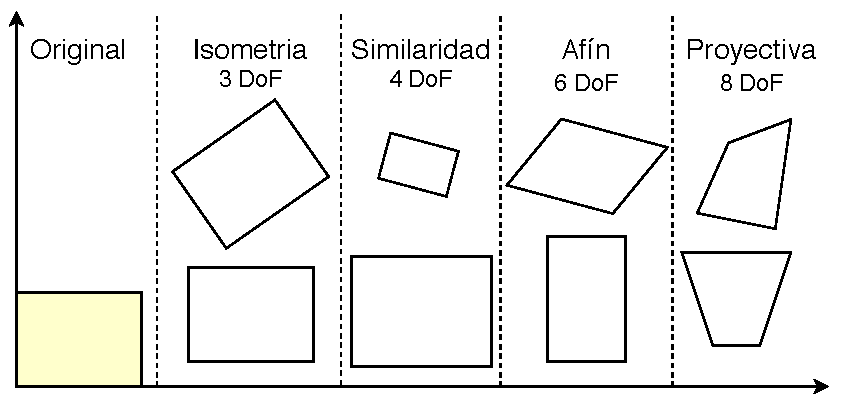
\includegraphics[width=14.5cm]{transformaciones.pdf}
	\caption[Tipos de transformaciones geométricas]{Tipos de transformaciones geométricas}
	\label{imagen:transformaciones}
\end{figure}

Las transformaciones proyectivas, al igual que las anteriores puede ser descompuesta en una serie de transformaciones de menor jerarquía, tal y como se muestra en la ecuación \ref{composicion-homografia} para la proyectiva.

\begin{equation}
\mathtt{H} = \mathtt{H}_\mathsf{S} \mathtt{H}_\mathsf{A} \mathtt{H}_\mathsf{P} = 
\begin{bmatrix}
{s\mathtt{R}}&{\vec{t}}\\
{\vec{0}}&{1}
\end{bmatrix}
\begin{bmatrix}
{\mathtt{K}}&{\vec{0}}\\
{\vec{0}}&{1}
\end{bmatrix}
\begin{bmatrix}
{\mathtt{I}}&{\vec{0}}\\
{\vec{v}}&{u}
\end{bmatrix} =
\begin{bmatrix}
{\mathtt{A}}&{\vec{t}}\\
{\vec{v}}&{u}
\end{bmatrix}
\label{composicion-homografia}
\end{equation}

Donde los sub-índices de las matrices corresponden con $\mathsf{S}$ = similaridad, $\mathsf{A}$ = Afín, $\mathsf{P}$ = Proyectiva. $\mathtt{R}$ es una matriz de rotación (no singular) $2\times2$,  $\mathtt{K}$ es una matriz $2\times2$ triangular superior normalizada tal que det$\mathtt{K}=1$ (para remover la escala y rotación), $\vec{t}$ es un vector de translación de 2 componentes, $\mathtt{I}$ es una matriz identidad $2\times2$, $\vec{v}$ es un vector de 2 componentes, $\mathtt{A}$ es una matriz no singular y $u\neq0$.

Las transformaciones proyectivas al estar compuestas por un grupo de transformaciones  también cumplen con las siguientes aserciones: \\
\textit{$\,$(i)$\,\,$}  El inverso de una homografía, es también una homografía.\\
\textit{(ii)} La composición de dos homografía es una homografía.\\
En base a esto, siempre es posible encontrar una matriz de transformación que pueda relacionar dos planos.


%%%%%%%%%%%%%%%%%%%%%%%%%%%%%%%%%%%%%%%%%%%%%%%%%%%%%%%%%%
\subsection{Estimación de Homografía}

El ultimo nivel de transformación estudiadas posee ocho grados de libertad (\textit{8-DoF}), con lo cual es posible estimar los parámetros de dicha transformación con tan solo 8 valores independientes. Por otro lado, conociendo que la homografía es una transformación que preserva la naturaleza de los objetos --- transforma puntos en puntos, lineas en lineas y planos en planos --, solo es posible relacionar dos imágenes mediante una homografía, siempre y cuando la escena que capturen corresponda con un plano. ver figura \ref{imagen:planos}.


\begin{figure}[h]
	\centering     %%% not \center
	\subfigure[]{\label{fig:a}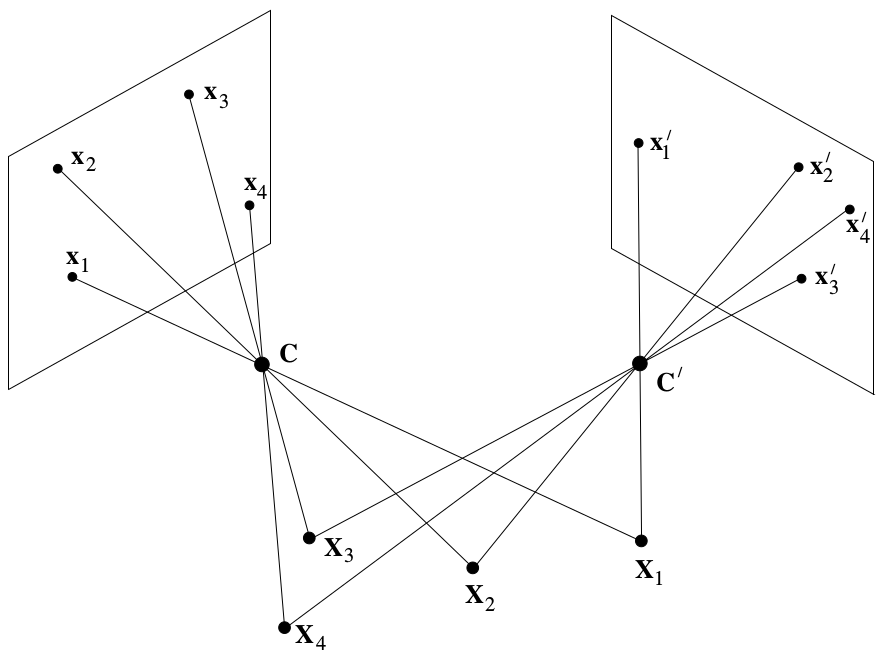
\includegraphics[width=.45\textwidth]{planos2}}\hspace{5mm}%}
	\subfigure[]{\label{fig:b}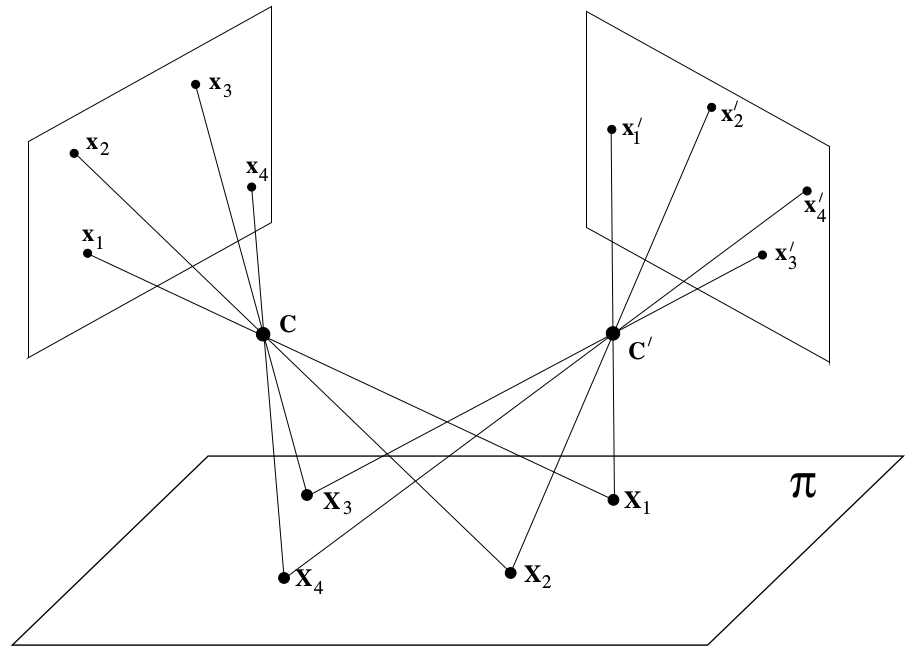
\includegraphics[width=.45\textwidth]{planos1}}
	\caption[Relacion de homografías]{Los puntos $\mathbf{C}$ y $\mathbf{C'}$ corresponden con los centros de la cámara en las distintas posiciones, Los puntos $\vec{x_i}$ y $\vec{x'_i}$ son la intersección de los puntos de la escena $\vec{X_i}$ en el plano de la imagen (formación de la imagen). Si la cámara se mueve no se podrá relacionar los planos de las imágenes con una homografía (izquierda), a menos que los puntos de la escena se encuentren todos en un mismo plano (derecha). Adaptado de \cite{zisserman}.}
	\label{imagen:planos}
\end{figure}

El primer paso para la estimación de la transformación consiste en encontrar 4 pares correspondientes de puntos, como cada punto en 2D posee 2-DoF ($x$ e $y$ del plano euclidiano de la imagen) con 4 puntos se tienen los 8-DoF. Luego por cada par de puntos se tienen (a partir de la ecuación \ref{matriz-perspectiva}) las siguientes relaciones: 
\begin{displaymath}
x'_i = \frac{x'}{w} = \frac{h_{11}x_i+h_{12}y_i+h_{13}}{h_{31}x_i+h_{32}y_i+h_{33}}, \qquad y'_i = \frac{y'}{w} = \frac{h_{21}x_i+h_{22}y_i+h_{23}}{h_{31}x_i+h_{32}y_i+h_{33}}
\end{displaymath}
Como se observa cada par de puntos genera dos ecuaciones lineales, mostradas a continuación luego de simplificar:
\begin{displaymath}
{x'_i ( h_{31}x_i+h_{32}y_i+h_{33} ) = h_{11}x_i+h_{12}y_i+h_{13}}
\end{displaymath}
\begin{displaymath}
{y'_i ( h_{31}x_i+h_{32}y_i+h_{33} ) = h_{21}x_i+h_{22}y_i+h_{23}}
\end{displaymath}
Escrito en forma matricial se puede expresar de la siguiente forma:
\begin{displaymath}
\mathtt{A}_i\vec{h}=\vec{0}
\end{displaymath}
Donde 
\begin{displaymath}
\mathtt{A}_i =
\begin{bmatrix}
-x_i&-y_i&-1&0&0&0&x'_ix_i&x'_iy_i&x'_i\\
0&0&0&-x_i&-y_i&-1&y'_ix_i&y_i'y_i&y'_i
\end{bmatrix}
\end{displaymath}
Y
\begin{displaymath}
\vec{h}^\mathtt{T} = (h_{11},\, h_{12},\, h_{13},\, h_{21},\, h_{22},\, h_{23},\, h_{31},\, h_{32},\, h_{33})
\end{displaymath}
Dado que 1 pareja arroja 2 ecuaciones lineales, 4 parejas arrojarían 8 ecuaciones, y se puede resolver el sistema para un factor multiplicativo dado por $h_{33}$ ($h_{33}=1$). La única restricción que tiene esta sistema de ecuaciones para asegurar un resultado único, es que no se tengan 3 puntos que residan en la misma linea. Con esto se tiene el siguiente sistema de ecuaciones:
\begin{displaymath}
\mathtt{A}\vec{h}=
\begin{bmatrix}
-x_1&-y_1&-1&0&0&0&x'_1x_1&x'_1y_1&x'_1\\
0&0&0&-x_1&-y_1&-1&y'_1x_1&y_1'y_1&y'_1\\
-x_2&-y_2&-1&0&0&0&x'_2x_2&x'_2y_2&x'_2\\
0&0&0&-x_2&-y_2&-1&y'_2x_2&y_2'y_2&y'_2\\
-x_3&-y_3&-1&0&0&0&x'_3x_3&x'_3y_3&x'_3\\
0&0&0&-x_3&-y_3&-1&y'_3x_3&y_3'y_3&y'_3\\
-x_4&-y_4&-1&0&0&0&x'_1x_1&x'_1y_1&x'_4\\
0&0&0&-x_4&-y_4&-1&y'_4x_4&y_4'y_4&y'_4
\end{bmatrix}
\begin{bmatrix}
h_{11}\\h_{12}\\h_{13}\\h_{21}\\h_{22}\\h_{23}\\h_{31}\\h_{32}\\h_{33}
\end{bmatrix}
= 0
\end{displaymath}
Añadiendo la condición de 	 $\left | \mathtt{H} \right | = 1$ para evitar la solución trivial $\vec{h}=0$. Luego se puede resolver mediante el método de descomposición en valores singulares SVD (del inglés: Singular Value Decomposition) con $\mathtt{A} = \mathtt{U}\mathtt{S}\mathtt{V}^\mathtt{T}$, donde $\mathtt{U}$ y $\mathtt{V}$ son matrices ortogonales; y $\mathtt{S}$ es una matriz formada con los valores singulares de $\mathtt{A}$ en su diagonal principal, ordenados en orden descendente. Finalmente el vector singular unitario correspondiente con el menor valor singular es la solución $\vec{h}$.

En este punto, la matriz encontrada se puede usar para transformar $\vec{x} \to \vec{x'}$, o bien se puede usar la inversa ($\mathtt{H^{-1}}$) para realizar el mapeo en sentido contrario.

Dada la naturaleza no plana de las escenas del mundo real, o bien debido a la inexactitud al medir los puntos cuando se captura una imagen, es muy poco probable que los puntos correspondientes radiquen en un mismo plano. Por otra parte es muy común que para aplicaciones de mapeo automático se cuenten con una gran cantidad de puntos correspondientes, con lo cual se tiene un sistema sobre determinado. En este caso es necesario realizar aproximaciones que permitan encontrar ya no la única homografía, sino la mejor, en función a los datos con los que se cuenten. Para esto es usual el uso de algoritmos que estiman la matriz buscando minimizar alguna función de coste.

Uno de los algoritmos mas usados para encontrar el mejor modelo está basado en el método RANSAC (del inglés: Random Sample Consensus), el cual es explicado a continuación.

%%%%%%%%%%%%%%%%%%%%%%%%%%%%%%%%%%%%%%%%%%%%%%%%%%%%%%%%%%
\subsubsection*{RANSAC}

Este es un método iterativo que permite calcular los parámetros de un modelo, a partir de un conjunto de datos que presentan valores atípicos. En nuestro caso, se tiene un conjunto sobre determinado de pares de puntos correspondientes, de los cuales se deben seleccionar los mejores 4 pares para estimar la mejor matriz de transformación, siendo la mejor aquella que logre minimizar la función de coste planteada.


Como ya se ha mencionado, las escenas que se estudian no son completamente planas, lo que provoca una inexactitud al estimar la transformación. Para lograr establecer un modelo, el método RANSAC considera solo los mejores datos que se logren ajustar a él, en este sentido se definen los \textit{inliers} y \textit{outliers}, donde los \textit{inliers} son aquellos valores que logran encajar en el modelo deseado, mientras que los \textit{outliers} son aquellos que no logran hacerlo. Por ejemplo: si se tienen un conjunto de puntos cuya distribución corresponden con el plano del suelo, estos serian los \textit{inliers}, y por otro lado aquellos puntos que no pertenecen a este plano serian los \textit{outliers}, ya sea por un emparejamiento erróneo o que pertenezcan a un segmento de distinta altitud de la escena. En la figura \ref{imagen:ransac} se ilustra esta distinción.

\begin{figure}[h]
	\centering
	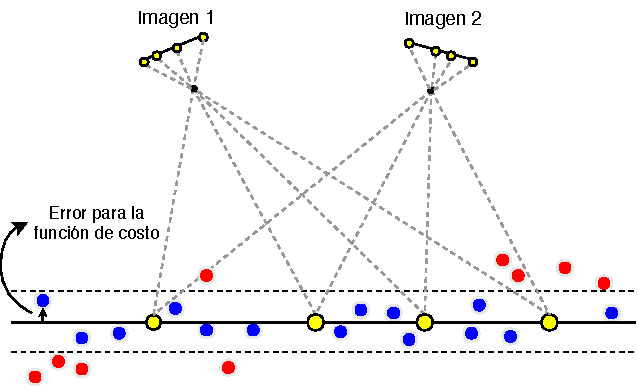
\includegraphics[width=14cm]{ransac.pdf}
	\caption[Mejor modelo - RANSAC]{Representación de un plano visto lateralmente. Los puntos amarillos corresponden con los utilizados para establecer el modelo (para calcular la matriz). Los puntos azules corresponden con los \textit{inliers}, mientras que los rojos con los \textit{outliers}. La distancia para la función de coste se mide desde cada punto hasta el plano modelo, considerando únicamente los \textit{inliers}.}
	\label{imagen:ransac}
\end{figure}

Ahora bien es necesario establecer la función de costo que buscará minimizar el algoritmo. En este caso se intenta disminuir el error cuadrático medio, donde el error es medido con la distancia de los puntos (inliers) correspondientes. Tal y como se observa en la figura \ref{imagen:ransac} el método RANSAC establece un perímetro que le permite distinguir \textit{inliers} de \textit{outliers}, ahora bien una vez se logran distinguir, el algoritmo solo considera los mejores para obtener el costo o peso asociado al modelo estimado, calculando para esto la distancia desde cada inlier hasta el plano. Este proceso se puede apreciar en el algoritmo \ref{ransac}.

\begin{figure}[hb]
	\centering
	\begin{minipage}{\linewidth}
		\begin{algorithm}[H] %or another one check
			\caption{Estimación de matriz de transformación RANSAC}
			\label{ransac}
			\SetAlgoLined
			\Begin{
				\While{No se llegue al maximo de iteraciones}
				{
					Se toman 4 parejas correspondientes\;
					Se calcula la matriz de homografía\;
					Se aplica la matriz sobre los puntos de origen\;
					Se calcula el error basado en distancia\tcp*{Solo considerando \textit{inliers}}
					\If{Error $<$ MejorError}
					{
						Guardar matriz como la mejor\;
						Guardar Error como el mejor\;
					}
				}
			}
		\end{algorithm}
	\end{minipage}
\end{figure}



%%%%%%%%%%%%%%%%%%%%%%%%%%%%%%%%%%%%%%%%%%%%%%%%%%%%%%%%%%
\section{Generación de sub-mosaicos}

El proceso mas simple para la generación de un mosaico consiste en añadir imágenes siguiendo los procesos planteados previamente, estableciendo el registro, y luego aplicando la matriz de transformación para lograr referenciarlas en el plano del mosaico. Ahora bien para el caso del primer par de imágenes, esta practica implica que se hallo la transformación desde la nueva añadida hacia la primera, tomando esta primera como plano de referencia. Esto se conoce como el proceso básico para la elaboración de mosaicos, en el cual se considera la primera imagen como referencia global para la construcción del mapa. La selección errónea de una imagen de referencia puede generar grandes distorsiones en el mosaico (especialmente para mapas grandes), y considerando el sistema simple, si no se cuenta con una primera imagen que se encuentre muy bien alineada con el plano del suelo, se comprometerá gravemente el resultado final del mosaico.

En busca de resolver este problema, \textit{Bellavia et. al.} en \cite{bellavia-ref,bellavia-ransac} plantean el modelo de sub mosaicos para lograr reducir el error geométrico producto de la mala selección de la imagen de referencia. Este sistema propone una estrategia para la selección del mejor plano de referencia que logre minimizar el error de distorsión, mediante la construcción de pequeños segmentos de mosaico que se alinean bajo el esquema básico, pero que poseen localmente poca distorsión geométrica.

\begin{figure}[h]
	\centering
	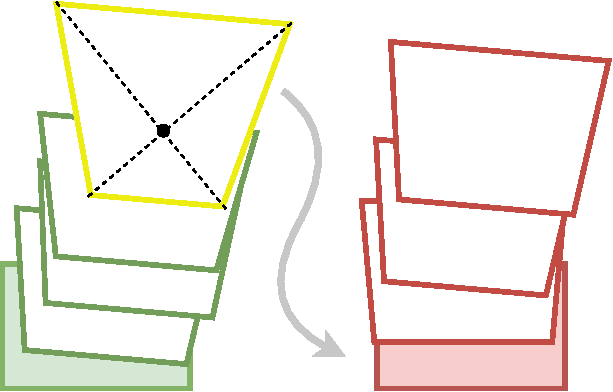
\includegraphics[width=0.6\linewidth]{submosaico.pdf}
	\caption[Generación de sub mosaicos]{Los cuadros verde y rojo son dos sub mosaico temporalmente continuos. El cuadro amarillo se convierte en el rojo relleno por presentar mucha distorsión.}
	\label{imagen:generacion-submosaico}
\end{figure}

La generación de los sub mosaicos consiste en el siguiente proceso: refiriéndonos a la figura \ref{imagen:generacion-submosaico}, se selecciona como referencia la primera imagen (cuadro verde relleno), se añaden imágenes al sub mosaico sucesivamente hasta que la siguiente presente mucha distorsión (cuadro amarillo), en este punto se crea un nuevo sub mosaico (cuadros rojos) y se añade aquella que presentó mucha distorsión como referencia para el nuevo sub mosaico. Donde el error es medido en función al área y el cociente entre semi-diagonales.

Siguiendo este proceso se van construyendo sub mosaicos hasta que no se cuenten con mas imágenes. Una vez se han creado todos los sub-mosaicos es necesario unirlos. En este punto cada sub mosaico considera la primera imagen como el plano de referencia, por lo tanto es necesario definir cual será la referencia bajo la cual éstos deben unirse. Para esto se utiliza la homografía que logre disminuir el error de distorsión sobre todos las imágenes del sub mosaico, esta transformación se define como \textit{homografía promedio}. El proceso para su obtención se detalla a continuación.



\subsection{Matriz de transformación promedio}\label{seccion-hpromedio}

Refiriéndonos a la figura \ref{imagen:homografia-promedio}, se observan los dos sub mosaicos que se desean unir, los cuales son temporalmente continuos, en la imagen superior se observan los sub mosaicos $S_j,\,S_k$ (marcos verde oscuro y verde claro) alineados y considerando la imagen de referencia del primero (verde lleno) como imagen de referencia global. En el segundo caso se muestran ambos alineados pero considerando la imagen de referencia del segundo (rojo lleno) como imagen de referencia global. 
\begin{figure}[h]
	\centering
	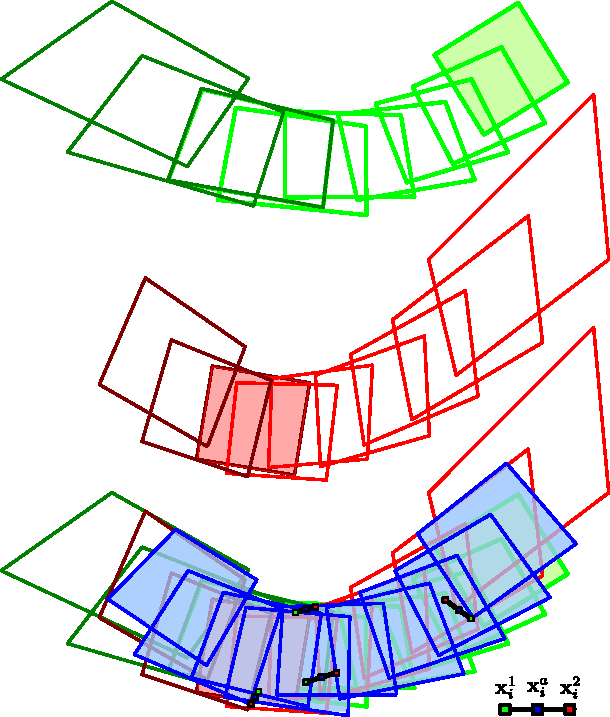
\includegraphics[width=8cm]{homografia-promedio.pdf}
	\caption[Estimación de homografia promedio]{Estimación de homografía promedio en base a 4 pares de puntos correspondientes, de \cite{bellavia-ref}}
	\label{imagen:homografia-promedio}
\end{figure}

Para encontrar la homografía promedio se aplica un algoritmo basado en el método RANSAC, el cual consiste en obtener 4 pares de puntos correspondientes ($x^1_i   \leftrightarrow x^2_i$) entre los dos sub mosaicos (verde y rojo) para un número fijo de iteraciones, seguidamente para dichos puntos se calcula el punto medio ($x^a_i$), luego se calcula la matriz que transforma los puntos del primer sub mosaico hacia los puntos medios ($x^a = \mathtt{H}x^1$), después se aplica la homografía en el primer sub mosaico y se obtiene la distorsión para dicha transformación. Finalmente la matriz que logre minimizar la distorsión global en el nuevo sub mosaico es seleccionada como la homografía promedio. Éste proceso se muestra mejor estructurado en el algoritmo \ref{homografia-promedio}.


\begin{spacing}{0.8}
	\begin{algorithm}[h] %or another one check
		\caption{Calculo de matriz de homografia promedio}
		\label{homografia-promedio}
		\SetAlgoLined
		\Begin{
			\While{no se alcanza el maximo de iteraciones}{
				Seleccionar 4 puntos aleatorios del primer sub-mosaico\;
				Seleccionar los 4 puntos correspondientes en el segundo sub-mosaico\;
				Salcular el punto medio para cada par de puntos correspondientes\;
				Calcular la transformacion desde los puntos del primer sub-mosaico hasta los puntos medios\;
				Aplicar transformacion en el primer sub-mosaico\;
				Calcular error de distorsión en el primer sub-mosaico\;
				\eIf{el error es menor que el mas bajo obtenido}{
					Guardar el error como el mas bajo\;
					Guardar la matriz de transformación como la mejor\;
				}{
				Restaurar valores del primer sub-mosaico\;
			}	
		}
		Aplicar mejor matriz al primer sub-mosaico\;
	}
\end{algorithm}
\end{spacing}

El criterio para determinar el grado de distorsión de la imagen se observa en la ecuación \ref{eq-error}, tal y como se propone en \cite{bellavia-ref}:

\begin{equation}
E = \max\limits_{I_i\in S_j\cap S_k} (E^O + E^C + E^A + E^\alpha)
\label{eq-error}
\end{equation}


Siendo $I_i$ una imagen perteneciente al par de sub mosaicos $S_j,S_k$. Con lo cual se considera la imagen que presente mas distorsión en el sub mosaico que se intenta unir. El error de cada tipo de error se encuentra normalizado en el rango $0\to 1$. 

\begin{figure}[h]
	\centering
	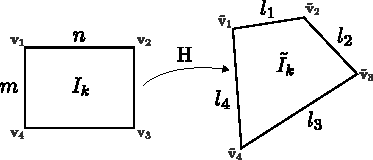
\includegraphics[width=0.6\linewidth]{distorsion.pdf}
	\caption[Distorsion de imagen]{Parámetros para el calculo de distorsión de una imagen, de \cite{bellavia-ref}}
	\label{imagen:distorsion}
\end{figure}

Considerado los parámetros mostrados en la figura \ref{imagen:distorsion} se describen los componentes del error en la ecuación \ref{eq-error}.

$E^O$ mide el error sobre lados opuestos de la imagen.
\begin{equation}
E^O = 1 - \frac{1}{2}  \left(  \frac{\min (l_1, l_3)}{\max (l_1, l_3)} +  \frac{\min (l_2, l_4)}{\max (l_2, l_4)} \right)
\end{equation}

$E^C$ mide el error sobre lados consecutivos, siendo $m > n$.
\begin{equation}
E^C = 1 - \frac{\min (r, \frac{m}{n})}{\max (r, \frac{m}{n})}
\end{equation}

Donde $r$ es el mínimo cociente entre lados consecutivos, expresado como:
\begin{displaymath}
r = \left( \frac{l_1}{l_2},\, \frac{l_2}{l_3},\, \frac{l_3}{l_4},\, \frac{l_4}{l_1} \right)
\end{displaymath}

$E^A$ mide el error del área
\begin{equation}
E^A = 1 - \frac{\min (A_{\tilde{I}_k},\, mn)}{\max (A_{\tilde{I}_k},\, mn)}
\end{equation}

$E^\alpha$ mide el error sobre los ángulos internos. 
\begin{equation}
E^\alpha = (\max (\cos\alpha_{12},\, \cos\alpha_{23},\, \cos\alpha_{34},\, \cos\alpha_{41}))^5
\end{equation}


\subsection{Selección de puntos característicos}\label{seleccion-grid}

Según se estudió en el método RANSAC, la estimación de una buena homografía depende de la distribución de los puntos en la escena. Es posible contar con una gran cantidad de puntos extraídos y emparejados en una sección de la escena que no corresponde con el mejor modelo del plano de ésta, lo que indica que la matriz de homografía se ajuste a dicha región por ofrecer menor peso en la función de coste. En cambio, el resultado esperado es que se tenga una mejor distribución de puntos en la escena de modo que se tenga una ponderación de igual magnitud para todas las regiones del suelo.

\begin{figure}[hb]
	\centering
	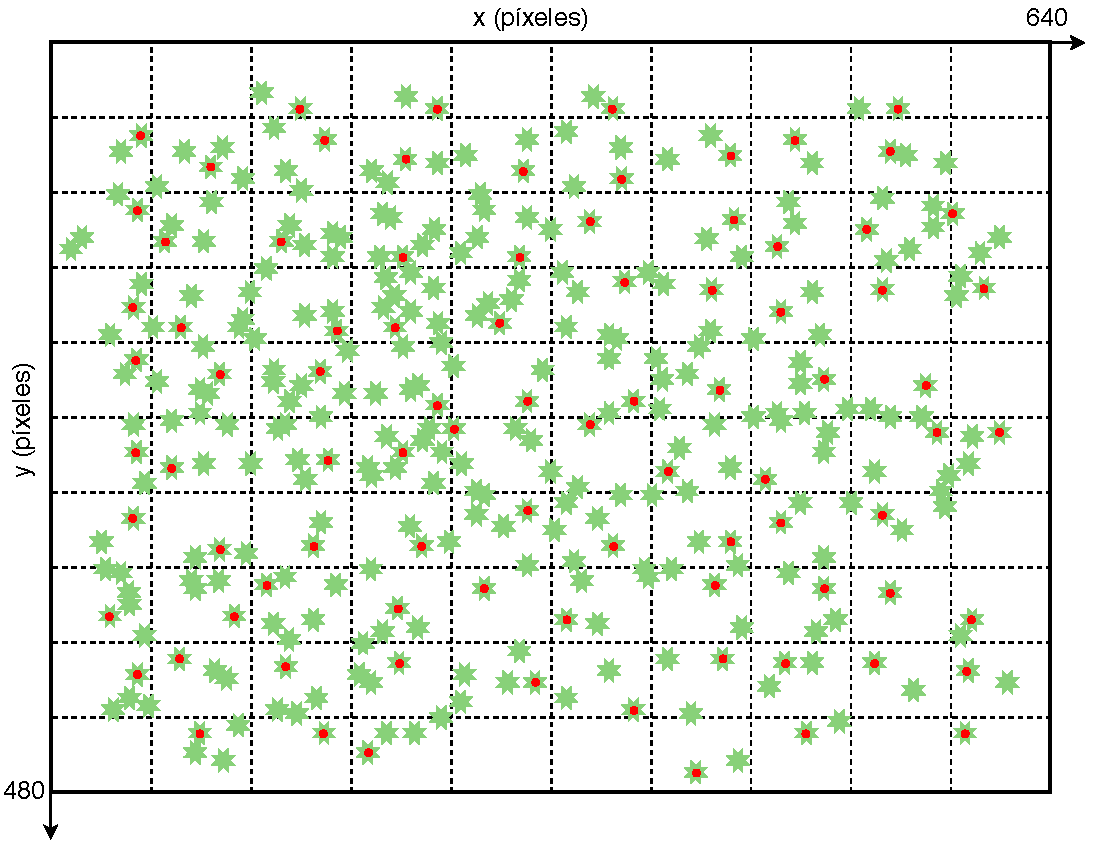
\includegraphics[width=0.8\linewidth]{celdas.pdf}
	\caption[Selección de mejores parejas]{Selección de mejores parejas en cada celda. Los puntos verdes corresponden con las parejas detectadas, y los puntos rojos serian las mejores pareas por cada celda.}
	\label{imagen:celdas}
\end{figure}

Para solucionar este problema, \textit{Eilbol et. al.} en \cite{grid} propone una segmentación espacial de los puntos emparejados entre dos imágenes, seguida de un proceso de selección con el objetivo de mejorar la distribución, y de esta forma ponderar de igual forma todas las secciones del plano. Básicamente el proceso consiste en dividir la imagen en $n\times m$ celdas, y por cada celda seleccionar la mejor pareja de puntos. Teniendo como resultado un máximo de $n\times m$ parejas entre imágenes. Esta división y selección se puede observar en la figura \ref{imagen:celdas}.

\begin{figure}[ht]
	\centering     %%% not \center
	\subfigure[30 inliers y 10 outliers (mejor modelo)]{\label{fig:grid-plano-a}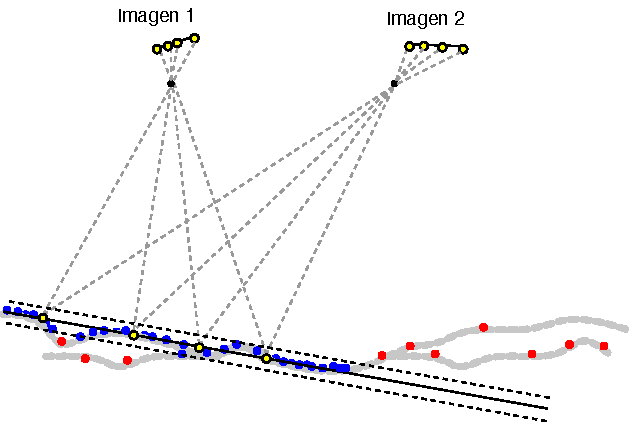
\includegraphics[width=0.8\textwidth]{grid-plano1.pdf}}%\hspace{10mm}%}
	
	\subfigure[10 inliers y 5 outliers (mejor modelo)]{\label{fig:grid-plano-b}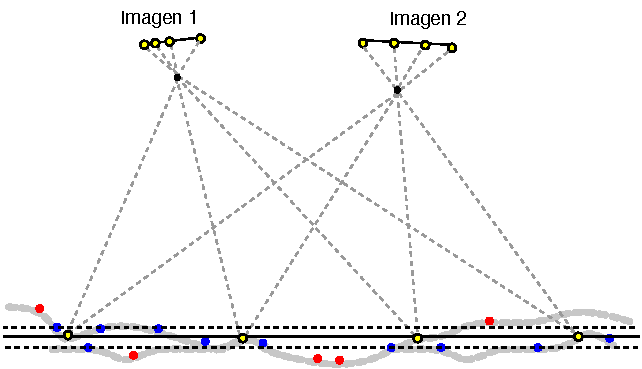
\includegraphics[width=0.8\textwidth]{grid-plano2.pdf}}
	\caption[Selección de mejores puntos, ejemplo con plano]{Ambas imágenes representan la vista lateral del plano de un suelo. En (a) se presenta el mejor modelo del plano con la cantidad original de parejas, mientras que en (b) se muestra el mismo proceso pero luego de haber seleccionado las parejas con enlace mas fuerte por cada región (según \ref{imagen:celdas}).}
	\label{imagen:grid-plano}
\end{figure}

Refiriéndonos a la figura \ref{imagen:grid-plano}, se observa como en \ref{fig:grid-plano-a} una fuerte aglomeración de parejas en una sección del plano (región con muchos puntos característicos) produce que la estimación de la matriz de homografía le asigne una alta ponderación al modelo del plano que se ajusta a esta región.

Por otro lado, en la figura  \ref{fig:grid-plano-b} se observa como se puede mejorar la estimación de la transformación, al seleccionar solo las mejores parejas por cada región, de esta forma la ponderación se distribuye de mejor manera a lo largo del plano del suelo.

\subsection{Seguimiento de puntos}\label{seguimiento-puntos}

Ya hemos visto el proceso simple de relacionar dos imágenes, donde luego de aplicar la transformación a la nueva imagen, ésta presentará cierto nivel de distorsión, afectando que imágenes siguientes logren establecer una relación robusta de puntos.

La primera propuesta consiste en buscar parejas de puntos correspondientes entre la nueva imagen y el mosaico (todas las imágenes añadidas previamente), pero esto trae consigo un bajo desempeño computacionalmente cuando se cuenta con un mosaico de gran tamaño. Si bien se puede restringir el área de búsqueda hacia el mínimo cuadro que encierra la ultima imagen transformada, el efecto de distorsión mencionado afecta la detección e identificación de puntos correspondientes.

\begin{figure}[h]
	\centering     %%% not \center
	\subfigure[]{\label{fig:ec-a}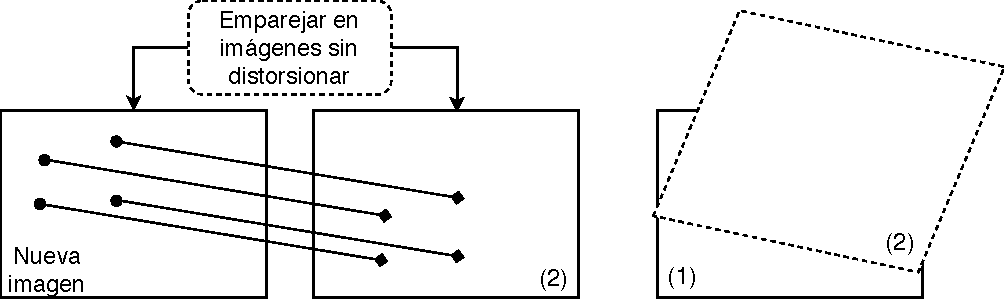
\includegraphics[width=.7\textwidth]{track1.pdf}}
	
	\subfigure[]{\label{fig:ec-b}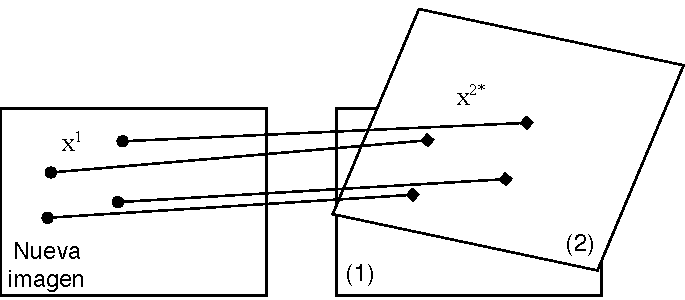
\includegraphics[width=.5\textwidth]{track2.pdf}}
	
	\caption[Seguimiento de puntos]{Seguimiento de puntos. En (a) se realiza la extracción y emparejamiento en las imágenes originales, luego los puntos detectados en la imagen (2) son transformados por la homografía que ubica esa imagen en el mosaico. finalmente en (b) se halla la matriz de transformación para la nueva imagen usando la nueva correspondencia.}
	\label{imagen:track}
\end{figure}

Para solucionar este problema se propone realizar una extracción de puntos característicos para todas las imágenes en su versión original, y una vez se conozca la matriz de transformación que ubica una imagen en el mosaico, se puede de igual forma transformar la ubicación de los puntos detectados hacia la nueva ubicación. Este proceso se encuentra ilustrado en la figura \ref{imagen:track}.

Definiendo $\vec{x}^1_i$ como los puntos que corresponden a la nueva imagen, $\vec{x}^2_i$ como los que corresponden a la última añadida con sus dimensiones y posición original, y $\vec{x}^{2*}_i$ serian aquellos de la ubicación en el mosaico. Primero se realiza la detección para encontrar la correspondencia $\vec{x}^1_i \leftrightarrow \vec{x}^2_i$, luego se transforman los puntos $x^2_i$ a su ubicación correspondiente en el mosaico $x^{2*} = \mathtt{H}^*\vec{x}^2$ ($\mathtt{H}^*$ conocida). Finalmente se encuentra la matriz de transformación para la nueva imagen con la siguiente relación: $\vec{x}^{2*} = \mathtt{H}\vec{x}^1$.



\subsection{Relación con vecinos}\label{seccion-vecinos}

Tal y como se ha planteado el proceso de registro hasta este punto, consiste establecer relación entre dos imágenes para estimar la homografía que permite alinearla. Esta practica es ideal cuando se tiene un movimiento continuo del robot al explorar el suelo, o bien cuando se tiene un bajo porcentaje de superposición (ver figura \ref{fig:vecinos1-a}), con lo cual se dificulta que una tercera imagen se relacione con la primera. Por otro lado, cuando estás condiciones no se cumplen, es necesario plantear soluciones que aprovechen toda la información posible de las imágenes para tener un sistema mucho mas robusto. En base a esto se planteó una técnica de búsqueda por vecinos para mejorar la etapa de registro, el proceso consiste en buscar relaciones de puntos entre imágenes que no sean temporalmente continuas, es decir, intentar relacionar una imagen con un grupo de todas aquellas inmediatamente anteriores, y que tengan información en común (intersección), a las cuales llamaremos imágenes vecinas (ver figura \ref{fig:vecinos1-b}).


\begin{figure}[h]
	\centering     %%% not \center
	\subfigure[]{\label{fig:vecinos1-a}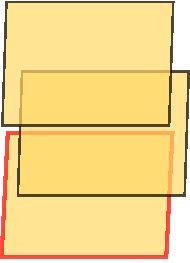
\includegraphics[height=.40\textwidth]{vecinos1.pdf}}\hspace{10mm}%}
	\subfigure[]{\label{fig:vecinos1-b}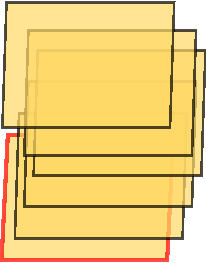
\includegraphics[height=.40\textwidth]{vecinos2.pdf}}
	\caption[Superposición de imagenes vecinas, mismo sentido]{En función a la ultima imagen añadida (superior), todas las imágenes con marco de color negro son considerados como vecinos. En el caso de la figura (b) una búsqueda en la que solo se considere la imagen anterior no aprovecha toda la información de aquellas con las que se intersecta}
	\label{imagen:vecinos1}
\end{figure}

Los casos presentados en la figura \ref{imagen:vecinos1} es aquel donde el movimiento del robot es monótono en un mismo sentido, pero también se puede presentar el caso en el cual este movimiento no se mantiene, con el cual una imagen distinta a la anterior puede aportar mas información para establecer la correspondencia con el mosaico. Este caso se ilustra en la figura \ref{imagen:cambio-sentido}, en \ref{fig:cambio-sentido-a} el movimiento es continuo hacia arriba, en \ref{fig:cambio-sentido-b} el movimiento cambia pero solo se considera la ultima imagen añadida, en \ref{fig:cambio-sentido-c} el sentido también cambia pero se consideran ambas imágenes para establecer la relación de homografía.

\begin{figure}[hb]
	\centering     %%% not \center
	\subfigure[]{\label{fig:cambio-sentido-a}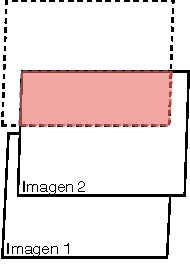
\includegraphics[width=.29\textwidth]{vecinos3.pdf}}\hspace{5mm}%}
	\subfigure[]{\label{fig:cambio-sentido-b}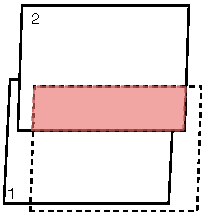
\includegraphics[width=.29\textwidth]{vecinos4.pdf}}\hspace{5mm}%
	\subfigure[]{\label{fig:cambio-sentido-c}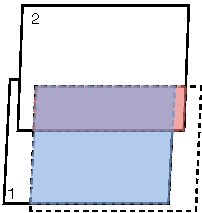
\includegraphics[width=.29\textwidth]{vecinos5.pdf}}
	
	\caption[Superposición de imágenes vecinas, cambio de sentido]{En rojo se muestra el área de superposición entre la nueva imagen (bordes punteados) y la última añadida (2), mientras que en azul se muestra aquella que comparte con una imagen no consecutiva (1).}
	
	\label{imagen:cambio-sentido}
\end{figure}

Considerando toda la información posible, se tiene un sistema que se adapta a una gran variedad de circunstancias que se pueden presentar en la exploración cuando se hace uso de un robot no tripulado. En este sentido se presenta en el algoritmo \ref{registro-completo} el proceso final para establecer la correspondencia de una imagen con el mosaico, es decir, el proceso de registro de imágenes.

\begin{figure}[h]
	\centering
	\begin{minipage}{.8\linewidth}
		\begin{algorithm}[H] %or another one check
			\caption{Relacionar imágenes}
			\label{registro-completo}
			\SetAlgoLined
			$I_{i+1}$ $\equiv$ Imagen nueva\;
			$I_{i}$ $\equiv$ ultima imagen añadida al mosaico\;
			$V_{i}$ $\equiv$ vecinos de $I_{i}$\;
			\While{puntos emparejados $\ge$ 4}{
				Emparejar puntos de $I_{i+1}$ con $I_{i}$\;
				\If{$I_{i}$ tiene vecinos}{
					\ForEach {vecino de $I_{i}$}{
						Emparejar puntos de $I_{i+1}$ con $V_{i}$\;
					}
				}
				descartar malos emparejamientos\;
				aplicar busqueda sectorizada\;
				\If{puntos totales emparejados $\le$ 3}{
					modificar criterio para descartar\;
					\If{criterio para descartar llega al minimo}{
						terminar \tcp*{no es posible emparejar imagen}
					}
				}
			}
		\end{algorithm}
	\end{minipage}
\end{figure}

%%%%%%%%%%%%%%%%%%%%%%%%%%%%%%%%%%%%%%%%%%%%%%%%%%%%%%%%%%%%%%%%%%%%%%%%
\section{Corrección euclidiana}\label{seccion-ec}

La concatenación de un gran grupo de imágenes en la formación de un mosaico, suele traer consigo un error de distorsión acumulado producto de la estimación de la mejor matriz de homografía, afectando en muchos casos el tamaño original de las imágenes. Para resolver este problema \textit{A. Elibol y R. Garcia} en \cite{elibol} proponen un método de corrección global basado en transformaciones de isometría.

Considerando que un robot de exploración (aéreo o submarino) con una cámara dirigida hacia abajo presenta pocas variaciones de rotación (ángulo de cabeceo y balanceo), además de intentar mantener una altura constante con el suelo, las transformaciones que describan su movimiento debería estar descrita por esos grados de libertad (rotación y translación, sin escala). En este sentido, se utiliza un modelo del sub mosaico que utiliza solamente transformaciones de isometría (ecuación \ref{matriz-isometria}). Aí mismo, al no contar con datos de navegación, como GPS que no está presente en aplicaciones bajo el agua, el método propuesto presenta una buena aproximación para reducir el error de tamaño en las imágenes del extremo del mosaico. Este proceso se encuentra listado a continuación, además se ilustra gráficamente en la figura \ref{imagen:correcion-e}.
\begin{figure}[h]
	\centering     %%% not \center
	\subfigure[]{\label{fig:ec-a}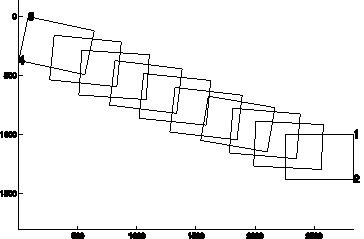
\includegraphics[width=.45\textwidth]{ec-1.pdf}}\hspace{5mm}%}
	\subfigure[]{\label{fig:ec-b}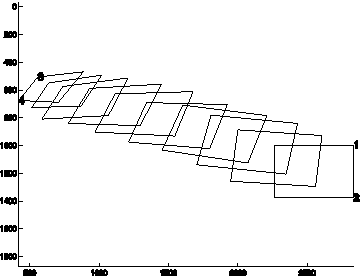
\includegraphics[width=.45\textwidth]{ec-2.pdf}}
	\subfigure[]{\label{fig:ec-c}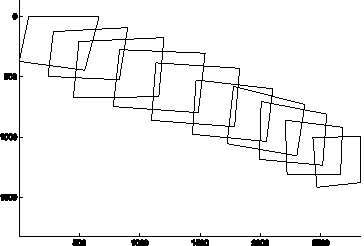
\includegraphics[width=.8\textwidth]{ec-3.pdf}}
	\caption[Correción euclidiana]{Correción euclidiana. (a) muestra el mosaico usando unicamente tranformaciones de isometría, (b) muestra el mosaico usando transformaciones de perspectiva, y (c) muestra el mosaico tras aplicar la corrección. de \cite{elibol}}
	
	\label{imagen:correcion-e}
\end{figure}
\begin{enumerate}%for capital roman numbers.
	\item Alinear imágenes usando transformaciones de Isometría
	\item Seleccionar coordenadas del borde del mosaico
	\item Alinear imágenes usando transformaciones de perspectiva
	\item Seleccionar mismas coordenadas del paso (2)
	\item Hallar homografía desde desde los puntos (2) hasta (4)
	\item Aplicar transformación a todas las imágenes del mosaico.
\end{enumerate}

Con respecto  a la selección de los puntos frontera del mosaico, el primer par se selecciona considerando aquellos de la primera imagen que se encuentren mas alejados del centro de la última, y para el ultimo par se consideran aquellos de la última imagen mas alejados del centro de la primera.

\section{Resultados}

En esta sección se presentan los resultados de aplicar los métodos descritos previamente, así como su análisis correspondiente. Debido a la estructura que presenta del proyecto, se muestran los resultados por separado de aquello módulos que se enfocan en el registro de pares de imágenes, mientras que para aquellos métodos que trabajan con múltiples imágenes se muestran resultados de algoritmos conjuntos.

\subsection*{Selección de puntos característicos}

A continuación se muestran los resultados de aplicar el método descrito en la 
sección \ref{seleccion-grid}. Para esto se estudia tanto analítica como visualmente el resultado de aplicar esta técnica. Al mismo tiempo se analiza el error de estimar una matriz de homografía según la distancia de los puntos correspondientes luego de aplicarla. 

Para cada conjunto se seleccionó un par de imágenes con las que se busca ejemplificar las mejoras que este método ofrece en la etapa de registro. Para una mejor visualización de los datos obtenidos, se propone un estudio de la distribución de las parejas según la distancia espacial que presenten, medida en píxeles. Conjuntamente se presenta para cada distribución las imágenes alineadas, donde se ilustran las parejas con mejor y peor distancia. Para lograr esta distinción se fijaron de color verde las pareas que presente mejor distancia, mientras que aquellas que tengan 3 veces mas distancia que la mejor, se denotan en color rojo. Para ambos casos se muestran de color azul los puntos correspondientes en la nueva imagen.

Por otra parte se analiza numéricamente el error en función a la distancia en las parejas de puntos. Para esto se estudia el error cuadrático medio, el cual mide el promedio de la diferencia entre el valor deseado y el obtenido, y se calcula usando la ecuación \ref{eqn-ECM}.
\begin{equation}\label{eqn-ECM}
	ECM = \frac{1}{n} \sum_{i}^{n} \left( \hat{\mathbf{D}} - \mathbf{D} \right)^2
\end{equation}

Donde $\hat{\mathbf{D}}$ es el valor deseado o esperado, y $\mathbf{D}$ es el valor obtenido, en este caso se trabaja con la distancia entre los puntos luego de aplicar la matriz de transformación. Lo ideal seria que al aplicar la matriz sobre los primeros puntos, con lo cual la distancia deseada entre ellos se considera igual a cero ($\hat{\mathbf{D}}$=0).

A continuación se muestran los resultados para imágenes de los conjuntos de datos \textit{Chuspa}, \textit{Mochima} y \textit{Grava}. Es importante considerar que para todos los casos se utilizó el extractor de puntos SIFT y el emparejador FLANN, también que las imágenes se trabajaron con una resolución de $640 \times 480$, a excepción del conjunto \textit{Grava} que presentan una resolución de $1280 \times 760$.

\subsubsection*{Chuspa}

En la figura \ref{imagen:grid:0233-match} se muestran las parejas detectadas, en la imagen superior se muestran todas las pareas posibles, mientras que en la inferior aquellas seleccionadas por el algoritmo propuesto. En la figura \ref{imagen:grid:0233-hist} se observan los histogramas de distribución según la distancia espacial. Finalmente en la figura \ref{imagen:grid:0233-align} se observa para cada caso las imágenes alineadas en un mismo plano.

\begin{figure}[h]
	\centering     %%% not \center
	\subfigure[]{\label{fig:hist1-a}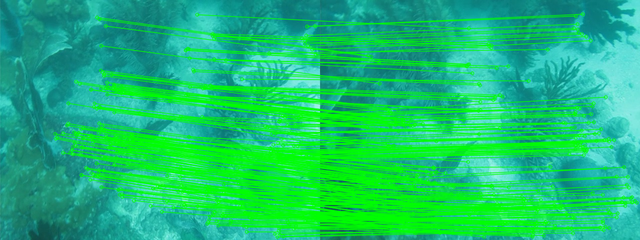
\includegraphics[width=1\textwidth]{resultados/grid/0233-3_4match}}\hspace{1mm}%}
	\subfigure[]{\label{fig:hist1-b}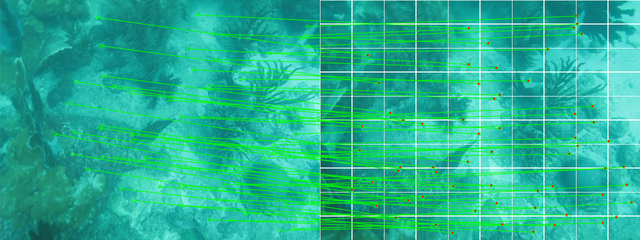
\includegraphics[width=1\textwidth]{resultados/grid/0233-3_4Gmatch}}
	
	\caption[Selección de puntos caracteristicos sobre el conjunto \textit{Chuspa}]{Selección de puntos característicos sobre el conjunto \textit{Chuspa}}
	\label{imagen:grid:0233-match}
\end{figure}

\begin{figure}[h]
	\centering     %%% not \center
	\subfigure[]{\label{fig:hist1-a}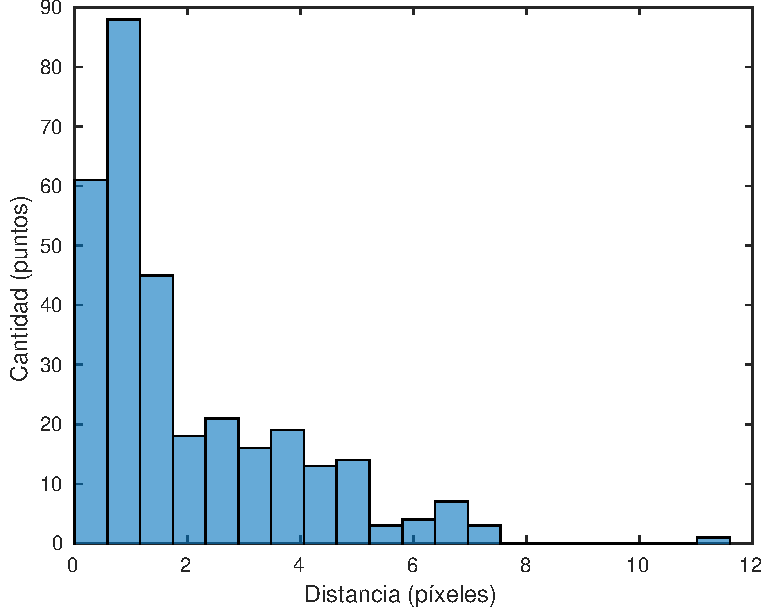
\includegraphics[height=.40\textwidth]{resultados/grid/0233-3_4.pdf}}\hspace{3mm}%}
	\subfigure[]{\label{fig:hist1-b}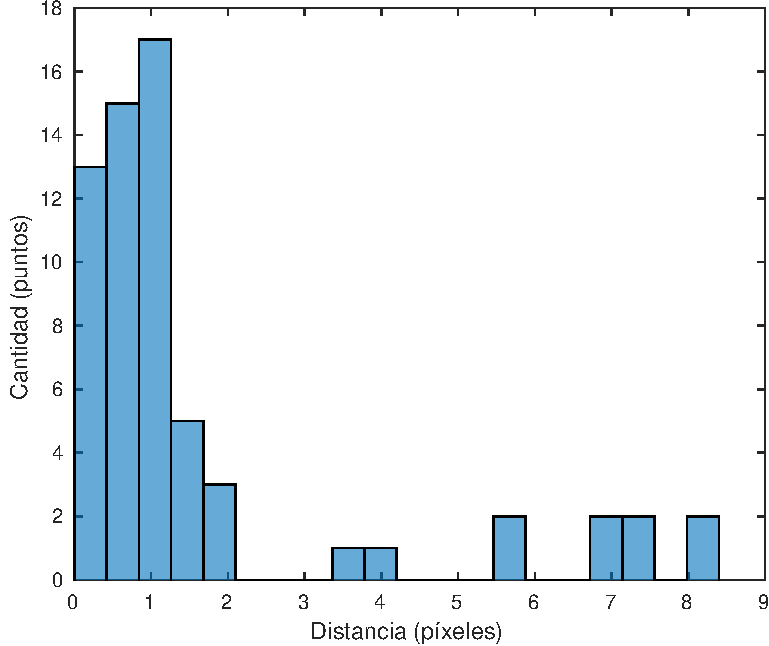
\includegraphics[height=.40\textwidth]{resultados/grid/0233-3_4G.pdf}}
	
	\caption[Histograma de la distancia de parejas sobre el conjunto \textit{Chuspa}]{Histograma de la distancia de parejas sobre el conjunto \textit{Chuspa}}
	\label{imagen:grid:0233-hist}
\end{figure}

\begin{figure}[h]
	\centering     %%% not \center
	\subfigure[]{\label{fig:hist1-a}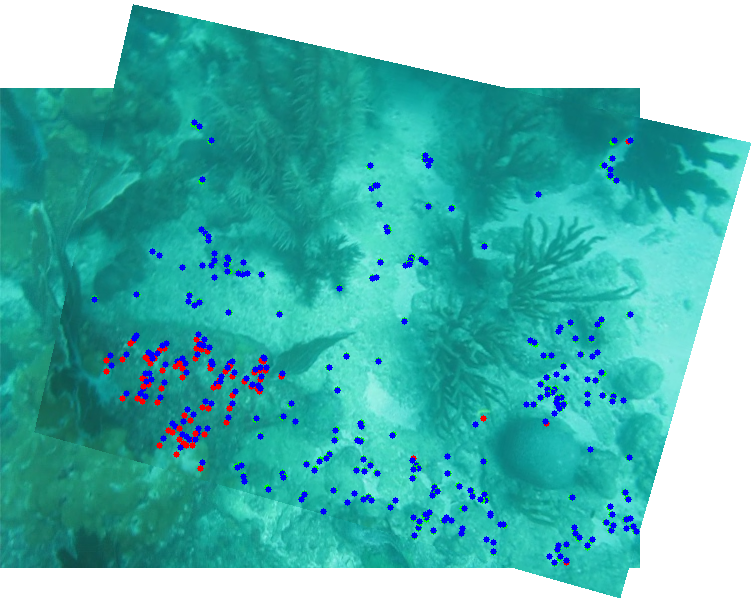
\includegraphics[width=.49\textwidth]{resultados/grid/0233-3_4.png}}\hspace{1mm}%}
	\subfigure[]{\label{fig:hist1-b}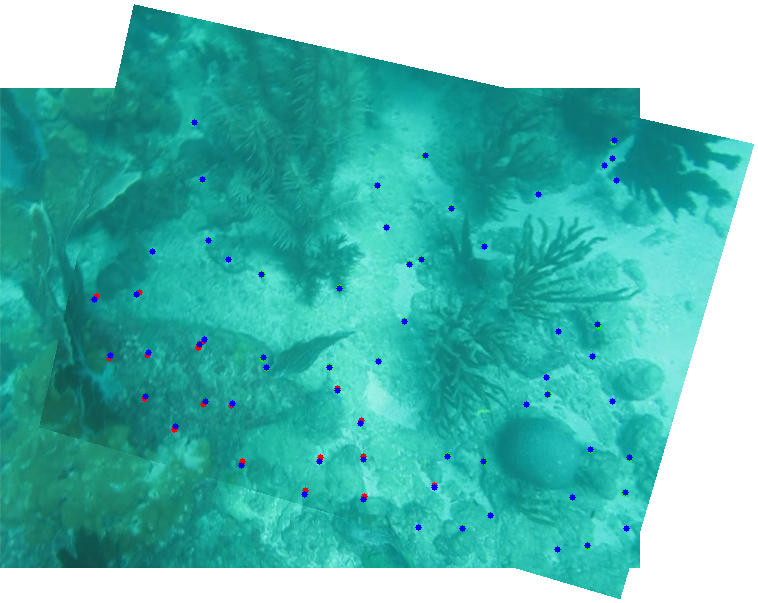
\includegraphics[width=.49\textwidth]{resultados/grid/0233-3_4G.png}}
	
	\caption[Distribucion de parejas en imágenes del conjunto \textit{Chuspa}]{Distribucion de parejas en imágenes del conjunto \textit{Chuspa}}
	\label{imagen:grid:0233-align}
\end{figure}


\subsubsection*{Grava}
En la figura \ref{imagen:grid:0233-match} se muestran las parejas detectadas, en la imagen superior se muestran todas las pareas posibles, mientras que en la inferior aquellas seleccionadas por el algoritmo propuesto. En la figura \ref{imagen:grid:0233-hist} se observan los histogramas de distribución según la distancia espacial. Finalmente en la figura \ref{imagen:grid:0233-align} se observa para cada caso las imágenes alineadas en un mismo plano.

\begin{figure}[h]
	\centering     %%% not \center
	\subfigure[]{\label{fig:hist1-a}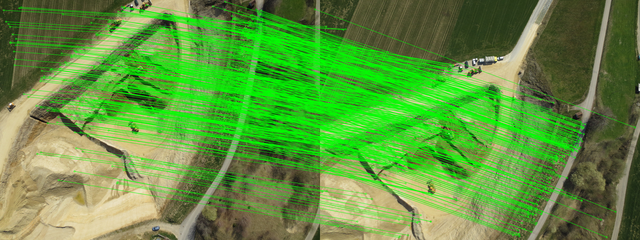
\includegraphics[width=1\textwidth]{resultados/grid/geomatch}}\hspace{1mm}%}
	\subfigure[]{\label{fig:hist1-b}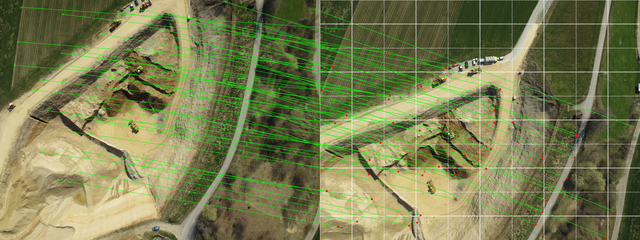
\includegraphics[width=1\textwidth]{resultados/grid/geomatchG}}
	
	\caption[Selección de puntos caracteristicos sobre el conjunto \textit{Grava}]{Selección de puntos característicos sobre el conjunto \textit{Grava}}
	\label{imagen:grid:geo-match}
\end{figure}

\begin{figure}[h]
	\centering     %%% not \center
	\subfigure[]{\label{fig:grid-geo-hist-a}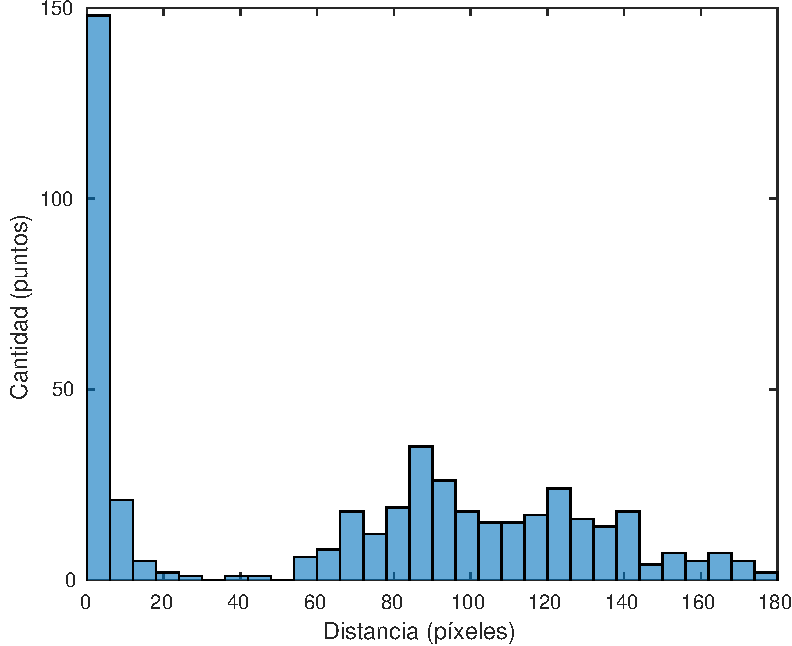
\includegraphics[height=.40\textwidth]{resultados/grid/geo-big-1_2.pdf}}\hspace{3mm}%}
	\subfigure[]{\label{fig:sub-geo-b}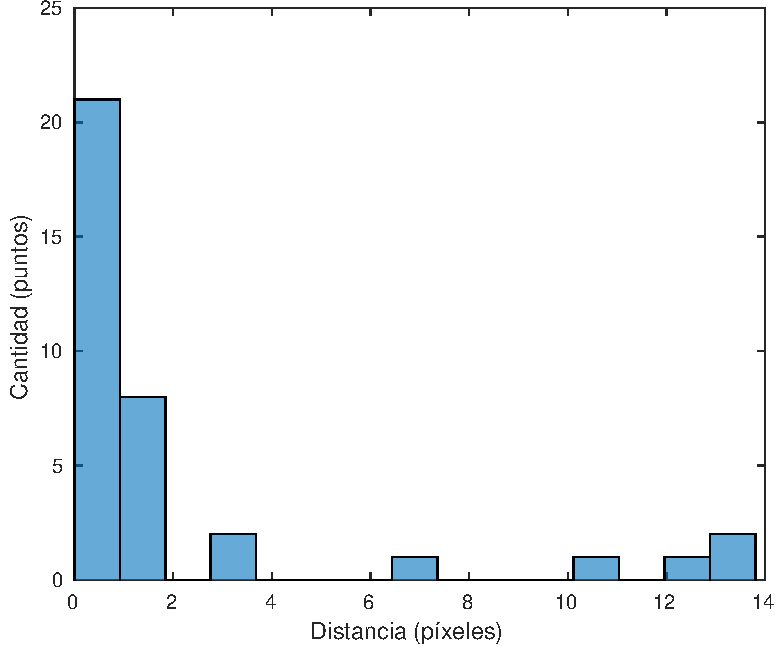
\includegraphics[height=.40\textwidth]{resultados/grid/geo-bigG-1_2.pdf}}
	
	\caption[Histograma de la distancia de parejas sobre el conjunto \textit{Grava}]{Histograma de la distancia de parejas sobre el conjunto \textit{Grava}}
	\label{imagen:grid:geo-hist}
\end{figure}
\begin{figure}[h]
	\centering     %%% not \center
	\subfigure[]{\label{fig:hist1-a}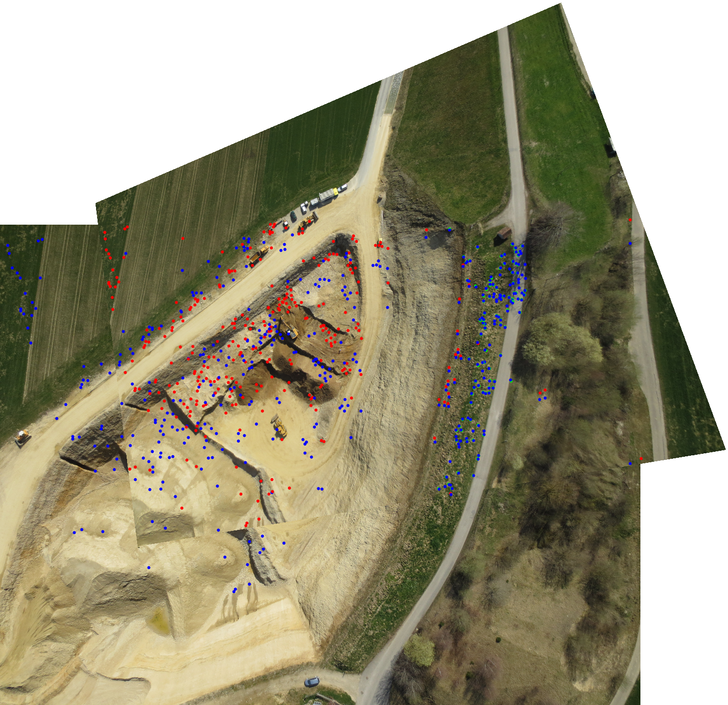
\includegraphics[width=.49\textwidth]{resultados/grid/geo.png}}\hspace{1mm}%}
	\subfigure[]{\label{fig:geo-align-b}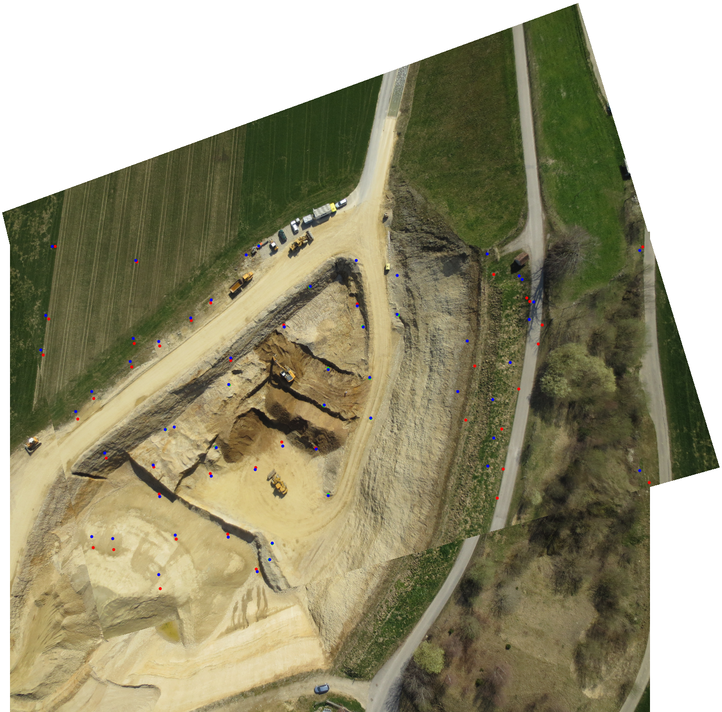
\includegraphics[width=.49\textwidth]{resultados/grid/geoG.png}}
	
	\caption[Distribucion de parejas en imágenes del conjunto \textit{Grava}]{Distribucion de parejas en imágenes del conjunto \textit{Grava}}
	\label{imagen:grid:geo-align}
\end{figure}



%\subsubsection*{Chuspa 2}

%En la figura \ref{imagen:grid:0234-match} se muestran las parejas detectadas, en la imagen superior se muestran todas las pareas posibles, mientras que en la inferior aquellas seleccionadas por el algoritmo propuesto. En la figura \ref{imagen:grid:0234-hist} se observan los histogramas de distribución según la distancia espacial. Finalmente en la figura \ref{imagen:grid:0234-align} se observa para cada caso las imágenes alineadas en un mismo plano.

%\begin{figure}[h]
%	\centering     %%% not \center
%	\subfigure[]{\label{fig:hist1-a}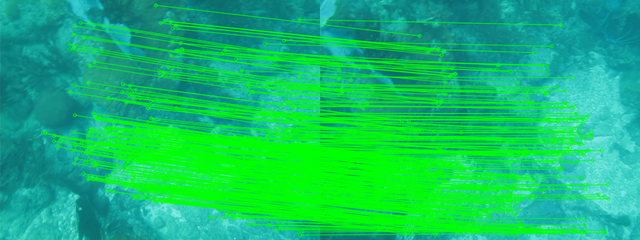
\includegraphics[width=1\textwidth]{resultados/grid/0234match}}\hspace{1mm}%}
%	\subfigure[]{\label{fig:hist1-b}\includegraphics[width=1\textwidth]{resultados/grid/0234matchG}}
	
%	\caption[Histogramas 1]{Histogramas 1}
%	\label{imagen:grid:0234-match}
%\end{figure}


%\begin{figure}[h]
%	\centering     %%% not \center
%	\subfigure[]{\label{fig:hist1-a}\includegraphics[height=.35\textwidth]{resultados/grid/0234-4_5.pdf}}\hspace{3mm}%}
%	\subfigure[]{\label{fig:hist1-b}\includegraphics[height=.35\textwidth]{resultados/grid/0234-4_5G.pdf}}
	
%	\caption[Histogramas 1]{Histogramas 1}
%	\label{imagen:grid:0234-hist}
%\end{figure}
%\begin{figure}[h]
%	\centering     %%% not \center
%	\subfigure[]{\label{fig:hist1-a}\includegraphics[width=.49\textwidth]{resultados/grid/0234-4_5.png}}\hspace{1mm}%}
%	\subfigure[]{\label{fig:hist1-b}\includegraphics[width=.49\textwidth]{resultados/grid/0234-4_5G.png}}
	
%	\caption[Histogramas 1]{Histogramas 1}
%	\label{imagen:grid:0234-align}
%\end{figure}


\subsubsection*{Mochima}

En la figura \ref{imagen:grid:0752-match} se muestran las parejas detectadas, en la imagen superior se muestran todas las pareas posibles, mientras que en la inferior aquellas seleccionadas por el algoritmo propuesto. En la figura \ref{imagen:grid:0752-hist} se observan los histogramas de distribución según la distancia espacial. Finalmente en la figura \ref{imagen:grid:0752-align} se observa para cada caso las imágenes alineadas en un mismo plano.

\begin{figure}[h]
	\centering     %%% not \center
	\subfigure[]{\label{fig:hist1-a}\includegraphics[width=1\textwidth]{resultados/grid/0752match}}\hspace{1mm}%}
	\subfigure[]{\label{fig:hist1-b}\includegraphics[width=1\textwidth]{resultados/grid/0752matchG}}
	
	\caption[Selección de puntos caracteristicos sobre el conjunto \textit{Mochima}]{Selección de puntos característicos sobre el conjunto \textit{Mochima}}
	\label{imagen:grid:0752-match}
\end{figure}

\begin{figure}[h]
	\centering     %%% not \center
	\subfigure[]{\label{fig:hist1-a}\includegraphics[height=.35\textwidth]{resultados/grid/0752-4_5.pdf}}\hspace{3mm}%}
	\subfigure[]{\label{fig:sub-0752-b}\includegraphics[height=.35\textwidth]{resultados/grid/0752-4_5G.pdf}}
	
	\caption[Histograma de la distancia de parejas sobre el conjunto \textit{Mochima}]{Histograma de la distancia de parejas sobre el conjunto \textit{Mochima}}
	\label{imagen:grid:0752-hist}
\end{figure}

\begin{figure}[h]
	\centering     %%% not \center
	\subfigure[]{\label{fig:hist1-a}\includegraphics[width=.49\textwidth]{resultados/grid/0752.png}}\hspace{1mm}%}
	\subfigure[]{\label{fig:hist1-b}\includegraphics[width=.49\textwidth]{resultados/grid/0752G.png}}
	
	\caption[Distribucion de parejas en imágenes del conjunto \textit{Mochima}]{Distribucion de parejas en imágenes del conjunto \textit{Mochima}}
	\label{imagen:grid:0752-align}
\end{figure}


\begin{table}[h]
	\centering
	\caption[Error cuadrático medio sobre la distancia de las parejas]{Error cuadrático medio sobre la distancia de las parejas}
	\label{tabla:ECM}
	\begin{tabular}{@{}lcccc@{}}
		\toprule
		\multicolumn{2}{l}{}           			 & Chuspa  & Grava & Mochima \\ \midrule
		\multirow{2}{*}{ECM} &\hfill Antes \hfill\vline& 3.69    &7664.50& 4.98    \\
							& Después      \vline& 3.46    & 20.06 & 3.92    \\
							
		\bottomrule 
	\end{tabular}
\end{table}

La distribución de puntos presentada en los histogramas nos revela información sobre la calidad de la transformación, donde el caso ideal se cumple cuando todos los puntos coinciden, es decir, todas las parejas tienen distancia igual a cero --- una sola barra agrupada a la izquierda ---, por lo tanto, buscar esta distribución debe ser el fin del presente algoritmo de selección, si bien no es posible lograr el caso ideal, se busca el mejor caso posible. 

Para realizar un correcto análisis de los datos presentados, es preciso estudiar la información de los histogramas en conjunto con las imágenes alineadas, de esta forma podemos apreciar la distribución de los puntos según la calidad a lo largo de las imágenes. Si bien es muy poco probable lograr el histograma ideal, es necesario contar con que los puntos agrupados hacia las distancias cortas (izquierda) se encuentren repartidos espacialmente por la mayor parte de las imágenes. Esto es para evitar que el modelo del plano resultante se ajuste dando mayor importancia a una pequeña región de la imagen.

Esta distribución indeseada puede traer consigo un problema común cuando se realiza emparejamiento simple (todas las parejas posibles), y es que la cantidad de parejas con poca distancia se encuentren ubicadas en una misa región, dando mayor importancia a dicha región para la estimación de la matriz de transformación. Si bien se suelen tener pocos puntos con mucha distancia, éstos suelen estar esparcidos por el resto de la imagen para estos casos. Dado que esta distribución en la imagen según la distancia no es posible visualizarla en el histograma, en las imágenes alineadas se facilita dicha distinción.

Considerando este factor, se puede observar en cada histograma que luego de aplicar la selección planteada, se muestra una fuerte agrupación de buenas parejas, y además se puede asegurar que la mayoría se encuentra distribuida a lo largo de toda la imagen. Para complementar el análisis, de forma que se pueda asegurar la misma o una mejor relación de parejas con corta y grandes distancias se presenta en la tabla \ref{tabla:ECM} el error cuadrático medio sobre cada par de imágenes antes y después de aplicar el método. De esta forma dada la reducción de muestras, se puede asegurar que el promedio de la calidad de emparejamientos luego de la selección mejora para los casos mostrados.

Un claro ejemplo de las mejoras que ofrece esta técnica la podemos apreciar con las imágenes del conjunto \textit{Grava}. En su primer histograma (figura \ref{fig:sub-geo-b}) se muestra una cantidad importante de parejas con media y elevada distancia (puntos alejados de la distancia cero), donde éstas corresponden con \textit{outliers} del modelo seleccionado. Si bien la cantidad  de \textit{inliers} (agrupación a la izquierda del histograma) es elevada, éstas se encuentran en una pequeña región de la imagen. Dicha distribución se aprecia en la figura \ref{imagen:grid:geo-align} con los parejas de puntos \textit{azul-verde}. 

Este error se produce ya que el terreno presente en la imagen esta compuesto por planos a distintas altitudes, con lo cual la matriz de transformación se ajusta a aquel plano que presente mayor cantidad de parejas, resultando en un par de imágenes con un fuerte error de alineación. 

El algoritmo propuesto logra reducir este error, tal y como se observa en la nueva distribución (histograma en la sub figura \ref{fig:sub-geo-b}) la mayoría de las parejas tienen una corta distancia, y además se asegura que éstos se encuentres dispersos por todas las celdas de la imagen. En la figura \ref{fig:geo-align-b} se puede observar la mejora en la alineación luego de aplicar la selección, si bien empeora un poco la alineación del antiguo plano modelo (plano presente a la derecha), el error global se minimiza en mayor medida. 

Analizando el histograma resultante para el resto de casos, se tiene una leve mejora en la distribución de parejas, logrando una reducción relativa de parejas con distancia elevada, y como se planteó anteriormente, se asegura también una distribución correcta de las nuevas parejas en toda la imagen, aseveración que no es posible realizar con el primer histograma. La reducción relativa de parejas con altas distancias se evidencia en la tabla \ref{tabla:ECM}, donde el error cuadrático medio se reduce para todos los casos evaluados. Esto indica que el promedio de las distancias (relación de cortas y largas distancias en las parejas) disminuye.

\subsection*{Seguimiento de puntos}

A continuación se muestran resultados obtenidos tras aplicar el método descrito en la sección \ref{seguimiento-puntos}. En primer lugar se presenta un resultado utilizando el conjunto \textit{ScottReef 25}, para el cual se observa en la figura \ref{fig:seg:SR-a} un conjunto de imágenes alineadas usando el método que consiste en establecer el registro entre la nueva imagen, y el mosaico previo, es decir, se buscan relaciones de puntos en el conjunto de imágenes previamente deformadas. Por otra parte en la figura \ref{fig:seg:SR-b} se aprecia el mismo conjunto de imágenes alineadas con el método propuesto, en el cual el registro se establece con las imágenes sin deformar, y realizando el seguimiento de puntos utilizando la matriz correspondiente.

Adicionalmente de la clara mejora en la transformación hallada, en el mosaico \ref{fig:seg:SR-a} no fue posible continuar alineando imágenes debido a la alta distorsión de los puntos característicos en la imagen. Caso contrario, en el nuevo mosaico es posible de continuar el crecimiento, conteniendo una imagen adicional, luego de la cual el proceso fue detenido intencionalmente. 

\begin{figure}[h]
	\centering     %%% not \center
	\subfigure[]{\label{fig:seg:SR-a}\includegraphics[width=0.30\textwidth]{resultados/seguimiento/SR-old}}\hspace{1mm}%}
	\subfigure[]{\label{fig:seg:SR-b}\includegraphics[width=0.30\textwidth]{resultados/seguimiento/SR-new}}
	
	\caption[Seguimiento de puntos: \textit{ScottReef 25}]{Mejora del seguimiento de puntos en conjunto \textit{ScottReef 25}. La figura (a) está compuesta por 5 imágenes, registro entre nueva imagen y mosaico (imágenes anteriores alineadas). La figura (b) está compuesta por 6 imágenes, registro entre nueva imagen e imagen anterior sin deformar}
	\label{imagen:seg:SR}
\end{figure}

Por otra parte, se presenta un resultado utilizando el conjunto \textit{Chuspa}. Similar al caso anterior, la cantidad de imágenes que se pueden añadir al mosaico utilizando el método de registro simple es muy limitada. Esto se puede observar en la figura \ref{fig:seg:0234-b}, ahí se presenta la máxima cantidad de imágenes que fue posible añadir (6 imágenes), mientras que en la figura \ref{fig:seg:0234-a} se muestran la cantidad de puntos que fue posible relacionar, en este caso el mínimo necesario (4 puntos). 

Luego de utilizar el método propuesto, la posibilidad de realizar el emparejamiento es muy elevada, ya que el registro entre imágenes se realiza siempre en las mejores condiciones (imágenes sin deformar). En este caso se tiene como resultado el de la figura \ref{fig:seg:0234-c}, donde se muestra un total de 19 imágenes, luego de las cuales el proceso fe detenido intencionalmente.

\begin{figure}[H]
	\centering
	\begin{varwidth}{0.49\linewidth}  % this is a must
		\centering
		\subfigure[]{\label{fig:seg:0234-a}\includegraphics[width=1\linewidth]{resultados/seguimiento/0234-old-match}}\\
		\subfigure[]{\label{fig:seg:0234-b}\includegraphics[width=1\linewidth]{resultados/seguimiento/0234-old}}
	\end{varwidth}
	\begin{varwidth}{0.50\linewidth}  % this is a must
		\centering
		\subfigure[]{\label{fig:seg:0234-c}\includegraphics[width=0.9\linewidth]{resultados/seguimiento/0234-new}}
		\color{white}
		\color{black}
	\end{varwidth}
	
	\caption[Mejora de aplicar seguimiento de puntos]{Incremento de la cantidad de imágenes al aplicar el método de seguimiento de puntos} 
	\label{imagen:seg:0234}
\end{figure}


\subsection*{Relación con vecinos}

A continuación se muestran resultados obtenidos tras aplicar el método descrito en la sección \ref{seccion-vecinos}. En este caso se presenta un mosaico utilizando imágenes del conjunto \textit{Mochima}. En la figura \ref{fig:vec:0752-a} se tiene un mosaico construido bajo el esquema simple, en el cual se relaciona la nueva imagen con la última añadida. Tal y como se observa en el mapa de la trayectoria mostrado en \ref{fig:vec:0752-c} hay un cambio en el recorrido --- La segunda imagen se posiciona debajo de la numero 1, luego la número 3 cambia el movimiento hacia arriba, donde el resto continúa con la trayectoria ---. Esto produce que la tercera imagen se relacione con la segunda solo bajo una pequeña área de superposición, produciendo el error de alineación (mostrada en la sección marcada).

En la figura \ref{fig:vec:0752-b} se muestra el resultado de un esquema que establece el registro de imágenes aprovechando la información de aquellas que se encuentren espacialmente cercanas. En este sentido, destacando la sección marcada es posible observar la mejora que éste método ofrece para este particular caso, logrando alinear correctamente la tercera imagen, utilizando la primera, con la cual comparte gran área de superposición.  



\begin{figure}[h]
	\centering     %%% not \center
	\subfigure[]{\label{fig:vec:0752-a}\includegraphics[width=0.29\textwidth]{resultados/vecinos/0752-old}}\hspace{1mm}%}
	\subfigure[]{\label{fig:vec:0752-b}\includegraphics[width=0.29\textwidth]{resultados/vecinos/0752-new}}\hspace{1mm}%}
	\subfigure[]{\label{fig:vec:0752-c}\includegraphics[width=0.29\textwidth]{resultados/vecinos/0752-newmap}}
	
	\caption[Busqueda de vecinos: \textit{Búsqueda por vecinos: \textit{Mochima}}]{Búsqueda por vecinos en mosaico compuesto por 8 imágenes. En (a) se muestra el registro de la nueva imagen con la anterior. En (b) el registro de la nueva imagen con las anteriores espacialmente cercanas. En (c) se muestra el mapa del mosaico en (b). Los puntos corresponden con el centro de la imagen, y el número con el orden de inclusión en el mosaico.}
	\label{imagen:vecinos:0752}
\end{figure}


\subsection*{Homografía promedio}

A continuación se muestran resultados obtenidos tras aplicar el método descrito en la sección \ref{seccion-hpromedio}. En el primer caso se muestra la unión de dos sub mosaicos del conjunto de imágenes \textit{Chuspa}. En la figura \ref{fig:h:0234-a} se observa dos sub mosaicos alineados en un mismo plano, y considerando la imágen de referencia del primero (cuadro marcado) como referencia global. Por otro lado en la figura \ref{fig:h:0234-b} se observa el mismo sub mosaico, pero considerando la imagen de referencia del segundo (cuadro marcado) como referencia global. 

Como se puede apreciar, ambos sub mosaicos presentan un elevado nivel de distorsión producto de la mala elección de la imagen de referencia. Ahora bien, al utilizar el método descrito anteriormente, es posible alinearlos logrando reducir el error de distorsión, tal y como se observa el resultado en la figura \ref{fig:h:0234-c}. 

En este caso el error fue obtenido según la ecuación \ref{eq-error}, donde se obtuvo un error de 2.56838 para el sub mosaico en \ref{fig:h:0234-a}, un error de 3.09599 para el sub mosaico en \ref{fig:h:0234-b}, y finalmente se logró reducir el error hasta 2.06248 para obtener el mosaico en \ref{fig:h:0234-c}.

\begin{figure}[h]
	\centering     %%% not \center
	\subfigure[]{\label{fig:h:0234-a}\includegraphics[width=0.32\textwidth]{resultados/hpromedio/0234-ref1}}\hspace{1mm}%}
	\subfigure[]{\label{fig:h:0234-b}\includegraphics[width=0.50\textwidth]{resultados/hpromedio/0234-ref2}}\hspace{1mm}%}
	\subfigure[]{\label{fig:h:0234-c}\includegraphics[width=0.66\textwidth]{resultados/hpromedio/0234-avg}}
	
	\caption[Homografía promedio: \textit{Mochima}]{Homografía promedio. (e) es el resultado luego de aplicar el método iterativo RANSAC sobre los sub mosaicos (a) y (b).}
	\label{imagen:avgh:0234}
\end{figure}

Otro resultado interesante se obtuvo utilizando imágenes del conjunto \textit{ScottReef 25}. En la figura \ref{fig:h:SR-a} se muestran dos sub mosaicos que consideran como referencia la imagen marcada con el cuadro verde, por otro lado el segundo sub mosaico está compuesto por una sola imágen, con lo cual se toma esta como referencia para realizar la segunda etapa de alineación, mosatrada en la figura \ref{fig:h:SR-b}. Finalmente, en la sigura \ref{fig:h:SR-c} se ilustra el par de sub mosaicos alineados según la homografía promedio que logra reducir en mayor medida el error de distorsión global. 

\begin{figure}[h]
	\centering     %%% not \center
	\subfigure[]{\label{fig:h:SR-a}\includegraphics[width=0.25\textwidth]{resultados/hpromedio/SR-ref0}}\hspace{1mm}%}
	\subfigure[]{\label{fig:h:SR-b}\includegraphics[width=0.20\textwidth]{resultados/hpromedio/SR-ref1}}\hspace{1mm}%}
	\subfigure[]{\label{fig:h:SR-c}\includegraphics[width=0.25\textwidth]{resultados/hpromedio/SR-avg}}
	
	\caption[Homografía promedio: \textit{ScottReef 25}]{Homografía promedio. }
	\label{imagen:avgh:SR}
\end{figure}

Un mosaico puede estar compuesto por una gran cantidad de sub mosaicos, si bien el proceso para unirlos ya se ilustró, se muestra el criterio para la selección sobre cuales se deben unir en primer lugar. Para esto se selecciona el par de sub mosaicos que presente mayor área de superposición a medida que se va construyendo. Es importante destacar que cuando se evalúan dos sub mosaicos ya corregidos, se considera la matriz de homografía promedio para determinar el área de superposición.

En la figura \ref{imagen:jerarquia0234} se observa la jerarquía con la que se seleccionan los sub mosaicos para ser alineados en el mosaico final. En este caso se redujo el criterio para detener el proceso de construcción de un sub mosaico, de modo que se cuente con una mayor cantidad de ellos y se ilustre de mejor manera el proceso.

Se muestran 9 sub mosaicos, compuestos por un total de  23 imágenes. Se observa como se unen los primeros cuatro sub mosaicos (desde izquierda a derecha) hasta un punto que se tiene otro par que presenta mayor área de superposición, con lo cual el proceso continúa con éstos. Siguiendo ese orden se tiene finalmente en la parte superior de la imagen el mosaico final.

\begin{figure}[H]
	\centering
	\includegraphics[width=1\linewidth]{resultados/jerarquia-reducido.pdf}
	\caption[Selección de sub mosaicos]{Jerarquía para selección de sub mosaicos}
	\label{imagen:jerarquia0234}
\end{figure}



\subsection*{Corrección euclidiana}

A continuación se muestran resultados obtenidos tras aplicar el método descrito en la sección \ref{seccion-ec}. Los cuales buscan reducir el error sobre el tamaño de las imágenes producto de la suma de errores al estimar la matriz de homografía. 

En primer lugar se muestra un resultado utilizando 12 imágenes del conjunto \textit{ScottReef 25}. En la figura \ref{imagen:ec:SR_1} se observa el mosaico construido únicamente con transformaciones de isometría. A la izquierda de observa el mosaico a color, y a la derecha el mapa con las coordenadas medidas en píxeles.

En el mapa (\ref{fig:ec:SRE-a}) se muestran los 4 puntos marcados con color verde que corresponden con el borde del mosaico. Por otro lado se muestra en la figura \ref{fig:ec:SRP-b} el mapa del mosaico creado usando transformaciones de perspectiva sin ningún tipo de correcciones. También se muestra en esa misma imagen en color rojo los 4 puntos correspondientes a los extremos del mosaico. Ahora bien, teniendo esta correspondencia de 4 pares de puntos, es posible hallar una matriz de transformación de perspectiva para lograr alinear los extremos del mosaico en \ref{fig:ec:SRP-b} con el \ref{fig:ec:SRP-a}. Luego de encontrar dicha transformación y aplicarla al segundo mosaico se obtiene el mosaico mostrado en la figura  \ref{imagen:ec:SR_3}.

Se puede observar en los tres mapas de coordenadas la ubicación relativa de los puntos frontera del mosaico. Considerando el origen en la esquina superior izquierda, se tiene que el mosaico construido con matrices de isometria no supera los 3.000 píxeles de longitud en el eje $y$, mientras que el construido con matrices de perspectiva logra superar los 11.000 píxeles. finalmente luego de la corrección la distancia entre los puntos del extremo logran coincidir en ambos mosaicos.


Se presenta otro resultado utilizando 30 imágenes del conjunto \textit{Chuspa}. Similar al caso anterior se muestran en las figuras \ref{imagen:ec:0234_1}, \ref{imagen:ec:0234_2} y \ref{imagen:ec:0234_3} el mosaico construido con matrices de isometría, matrices de perspectiva y el mosaico corregido respectivamente.

\begin{figure}[H]
	\centering     %%% not \center
	\subfigure[]{\label{fig:ec:SRE-a}\includegraphics[height=0.6\textwidth]{resultados/ec/SR-e}}\hspace{1mm}%}
	\subfigure[]{\label{fig:ec:SRE-b}\includegraphics[height=0.6\textwidth]{resultados/ec/SR-emap}}\hspace{1mm}%}
	\caption[Mosaico con transformaciones de Isometria]{Mosaico con transformaciones de Isometria del conjunto \textit{ScottReef 25}}
	\label{imagen:ec:SR_1}
\end{figure}

\begin{figure}[H]
	\centering     %%% not \center
	
	\subfigure[]{\label{fig:ec:SRP-a}\includegraphics[height=0.6\textwidth]{resultados/ec/SR-f}}\hspace{1mm}%}
	\subfigure[]{\label{fig:ec:SRP-b}\includegraphics[height=0.6\textwidth]{resultados/ec/SR-fmap}}\hspace{1mm}%}
	
	\caption[Mosaico con transformaciones de Perspectiva]{Mosaico con transformaciones de Perspectiva del conjunto \textit{ScottReef 25}}
	\label{imagen:ec:SR_2}
\end{figure}

\begin{figure}[H]
	\centering     %%% not \center
	\subfigure[]{\label{fig:ec:SRC-a}\includegraphics[height=0.6\textwidth]{resultados/ec/SR-ec}}\hspace{1mm}%}
	\subfigure[]{\label{fig:ec:SRC-b}\includegraphics[height=0.6\textwidth]{resultados/ec/SR-ecmap}}
	\caption[Mosaico con corrección de Isometria]{Mosaico con corrección de Isometria del conjunto \textit{ScottReef 25}}
	\label{imagen:ec:SR_3}
\end{figure}


\begin{figure}[H]
	\centering     %%% not \center
	\subfigure[]{\label{fig:ec0234-a}\includegraphics[height=0.60\textwidth]{resultados/ec/0234-e}}\hspace{1mm}%}
	\subfigure[]{\label{fig:ec0234-b}\includegraphics[height=0.60\textwidth]{resultados/ec/0234-emap}}\hspace{1mm}%}
	\caption[Mosaico con transformaciones de Isometria]{Mosaico con transformaciones de Isometria del conjunto \textit{Chuspa}}
	\label{imagen:ec:0234_1}
\end{figure}

\begin{figure}[H]
	\centering     %%% not \center
	
	\subfigure[]{\label{fig:ec1-a}\includegraphics[height=0.6\textwidth]{resultados/ec/0234-f}}\hspace{1mm}%}
	\subfigure[]{\label{fig:ec1-b}\includegraphics[height=0.6\textwidth]{resultados/ec/0234-fmap}}\hspace{1mm}%}
	
	\caption[Mosaico con transformaciones de Perspectiva]{Mosaico con transformaciones de Perspectiva del conjunto \textit{Chuspa}}
	\label{imagen:ec:0234_2}
\end{figure}

\begin{figure}[H]
	\centering     %%% not \center
	\subfigure[]{\label{fig:ec2-a}\includegraphics[height=0.65\textwidth]{resultados/ec/0234-ec}}\hspace{1mm}%}
	\subfigure[]{\label{fig:ec2-b}\includegraphics[height=0.65\textwidth]{resultados/ec/0234-ecmap}}
	\caption[Mosaico con corrección de Perspectiva]{Mosaico con corrección de Perspectiva del conjunto \textit{Chuspa}}
	\label{imagen:ec:0234_3}
\end{figure}

Con respecto a las coordenadas del mosaico corregido, si bien la posición de los puntos con coincide totalmente, la distancia entre estos si lo hace. Esto es debido a un desplazamiento del mosaico corregido para poder definirlo completamente con coordenadas positivas. 

\section{Resumen}

En este capítulo se describieron los principios básicos que permiten alinear imágenes bajo un mismo sistema de referencia, utilizando la información que proveen los extractores de características locales. Para esto se introdujeron los distintos niveles de transformaciones geométricas en base a los grados de libertad que ofrece cada una y a la cantidad de variables que preservan de las imágenes, además del proceso para su obtención.

Luego se introdujeron los diversos problemas que se tienen al realizar la alineación bajo el esquema mas simple. En función a esto se buscó resolver errores producidos por la mala selección de la imagen de referencia, por realizar el registro con las imágenes deformadas, y por solo considerar la ultima imagen añadida para establecer la referencia necesaria.

Finalmente se presentaron los resultados que validan los métodos descritos, obteniendo de estos mejoras claras sobre la geometría del mosaico y la robustez para su construcción.



\chapter{Unión de imágenes}
\label{capitulo5}
\lhead{Capítulo 5. \emph{Unión de imágenes}}


\section{Introducción}
El objetivo final de la creación de un mosaico, es lograr un mapa que represente de la mejor forma la trayectoria recorrida. Esto es, que sea visualmente congruente y que no presente ningún tipo de discontinuidades de modo que todo parezca una misma imagen. De las primeras etapas se manifiestan muchos errores producto de los problemas ya planteados, si bien a lo largo del proceso éstos se intentan reducir lo mas posible, siempre es necesaria la etapa final de fusión para lograr los objetivos propuestos.

En esta sección se describen los algoritmos utilizados para lograr fusionar las imágenes del mosaico. Como ya se especificó, fueron seleccionados aquellos que presentaron resultados importantes en diversos estudios externos, y se implementaron en conjunto para lograr resultados mucho mas robustos. Estos se detallan a continuación en el orden de aplicación sobre el mosaico: linea de corte, ajuste de color y finalmente la fusión ponderada.

Por ultimo, al final del capítulo se muestran los resultados con su respectivo análisis de aplicar cada uno de los algoritmos aquí descritos.
\clearpage


\section{Linea de costura}\label{seccion-corte}

Este es el primer algoritmo aplicado al mosaico luego de todas las correcciones geométricas, ya que el resto de métodos requieren conocer de antemano los límites de cada imagen. 
A diferencia de los anteriores, este tipo de algoritmos es el único que toma en cuenta la información que comparten las imágenes en el área que tienen en común, con lo cual su implementación logra corregir la mayor cantidad de imperfecciones. 


\subsection{Modelo por grafo}

Este es un método derivado de la teoría de grafos, donde la idea es separar un grafo con conexiones simples en dos grafos separados con un mínimo costo de separación. Se define un grafo $\mathcal{G} = \langle \mathcal{N}, \mathcal{E} \rangle$ como un conjunto de nodos $\mathcal{N}$, conectados por enlaces $\mathcal{E}$. Cada enlace conecta dos nodos y tiene asociado un costo o peso $\mathcal{W}(p, q) \,\, p,q \in \mathcal{N}$ --- cuando se habla de conexión simple, se refiere a que el costo en los enlaces está asociado para ambas direcciones $\mathcal{W}(p, q) = \mathcal{W}(p, q)$ ---. Se dice que dos grafos están separados si no se tiene ningún enlace que conecte dos nodos entre los grafos. Definimos $\mathcal{S}$ y $\mathcal{T}$ como los grafos separados que se tienen luego de aplicar el corte en $\mathcal{G}$. El método para determinar el mejor corte, se basa en encontrar el camino entre los enlaces que logra separa un grafo en dos, con el mínimo costo de corte \cite{graph-cut}, donde el costo del corte es la suma de los pesos de todos los enlaces del camino seleccionado.

En el conjunto de nodos presentes en el grafo se cuentan con dos especiales llamados nodos terminales, el inicio ($\mathtt{I}$) y el final ($\mathtt{F}$), donde el resto de píxeles en la imagen corresponden con un nodo no terminal. En aplicaciones de visión por computadora, cuando se desea unir dos imágenes en una región de intersección, lo que se busca es lograr un etiquetado de píxeles que permita distinguir que nodos corresponden a cada imagen en el área de intersección.

Se presenta en la ecuación \ref{funcion-corte} la función de coste que etiqueta los nodos, y minimiza el costo del corte.
\begin{equation}
C(f) = \sum_{_p\in \mathcal{N}}^{} D_p(f_p) + \sum_{_p,_q \in \mathcal{N} - \{\mathtt{I},\mathtt{F}\}}^{} \mathcal{W}_p,_q (f_p, f_q)
\label{funcion-corte}
\end{equation}
Donde $p$ es un nodo que pertenece al conjunto de nodos no terminales $\mathcal{N} - \{\mathtt{I},\mathtt{F}\}$. El término $D_p(f_p)$ es el costo de asignar una etiqueta $f_p$ ($f_p \in \{0,\,1\}$) al nodo $p$ --- en este caso una etiqueta binaria, asociando el píxel a una imagen u otra ---. El término $\mathcal{W}_{p,q} (f_p, f_q)$ es el costo de asociar una etiqueta al nodo $p$ y una distinta al nodo $q$.

Una gran diferencia de intensidades entre píxeles adyacentes representa un fuerte indicador de la existencia de un borde o contorno entre dos objetos, es decir, que el costo de un enlace se puede definir como el inverso de la diferencia entre la intensidad de los píxeles que conecta. Siendo $I(p)$ la intensidad de un píxel $p$, se defina el coso de cada enlace como:
\begin{equation}
\mathcal{W}_p,_q = 255 - |I(p) - I (q)|
\label{costo-corte}
\end{equation}
Si bien se consideran los parámetros necesarios con esa función, se obtienen resultados mucho mas robustos usando una función exponencial \cite{graph-opencv}:
\begin{equation}
\mathcal{W}_p,_q = e^{\left(\frac{255-|I(p) - I (q)|}{2 \sigma}  \right) }
\label{costo-corte}
\end{equation}
Donde $\sigma$ es la desviación estándar de la imagen, y siendo válido para los casos en los que $f_p \neq f_q$. Esto indica que dos nodos continuos pertenecen a distintos grafos ($\mathcal{S,T}$) y a su vez que son separados por la linea de corte.

\begin{figure}[h]
	\centering
	\includegraphics[width=1\linewidth]{grafo-completo.pdf}
	\caption[Corte por grafo]{De izquierda a derecha: imagen original, creación de nodos y enlaces, se asignan los pesos y se halla la linea de corte, finalmente se binariza la imagen según las etiquetas para crear una mascara.}
	\label{imagen:grafo}
\end{figure}

Refiriéndonos a la figura \ref{imagen:grafo}, se observa el proceso de modelar una imagen mediante un grafo con conexiones simples y usando un esquema de 4 vecindad --- 4 vecindad solo considera a los píxeles superior, inferior y laterales como vecinos ---, donde cada cuadro está compuesto por el inverso de la diferencia de intensidades entre dos imágenes, representado en escala de grises. Al final se tiene una imagen compuesta por dos grafos separados, donde $\mathtt{I} \in \mathcal{S}$ y $\mathtt{F} \in \mathcal{T}$ donde a cada nodo del grafo se le asigna un valor binario dependiendo de la etiqueta resultante el algoritmo de minimización del costo de corte.


\section{Corrección de color}\label{seccion-color}
Cuando se tienen imágenes capturadas desde distintos puntos de vista, se suelen tener en la composición final cambios de intensidades, debido a cambios de exposición de luz en la escena. Por ellos es necesario implementar algoritmos que logran reducir la diferencia de intensidades y color entre los bordes de las imágenes. Para esto se implementa un algoritmo de mapeo de color llamado método de \textit{Reinhard} \cite{reinhard} que trabaja en el espacio de color CIELAB, descrito a continuación. 

\subsubsection*{Espacio de color CIELAB}

Conocido en ocasiones con el nombre de l*a*b, es un espacio derivado del \textit{CIE 1931 XYZ}, creado por la comisión internacional de la iluminación CIE (del francés: Comission Internationale de l'Éclairage).

\begin{figure}[h]
	\centering     %%% not \center
	\subfigure[]{\label{fig:lab-a}\includegraphics[width=.42\textwidth]{lab1}}
	\subfigure[]{\label{fig:lab-b}\includegraphics[width=.50\textwidth]{lab2}}
	
	\caption[Espacio de color CIELAB]{Espacio de color CIELAB. En (a) se aprecia el diagrama tridimensional, mientras que en (b) una vista superior del rango de colores con luminancia fija.}
	\label{imagen:lab-color}
\end{figure}

Este es un espacio de color tridimensional descrito por los ejes $a$, que extiende desde verde ($-a$) hasta rojo ($+a$), el eje $b$ que se extiende desde azul ($-b$) hasta amarillo ($+b$), y la luminancia $l$ que varia desde negro ($-l$) hasta blanco ($+l$). Esta representación se puede observar en la figura \ref{imagen:lab-color}.

Debido a que la cantidad de valores para representar los colores en este espacio es menor que en RGB, es mas rápido hacer correcciones de color en LAB, ya que un cambio en la cantidad de valor de una variable produce un cambio con importancia visual. Además de permitir trabajar la iluminación de la imagen por separado de los colores.

\subsection{Método de Reinhard}
El objetivo de esta transformación de color es lograr que la distribución de los puntos en el espacio de color LAB se transfieran entre imágenes. Para esto se utiliza la información de la media y desviación estándar sobre cada canal (L, A y B).

Para un par de imágenes $I$ e $I^*$, donde $I$ es la imagen origen e $I^*$ es la imagen que se quiere corregir, se calcula la media y desviación estándar para cada canal.
\begin{align*}
&{\langle l \rangle} \hspace{0.55cm} {\langle l^* \rangle}  &{ \sigma_l } \hspace{0.5cm} { \sigma^*_l } \\
&{\langle a \rangle} \hspace{0.48cm} {\langle a^* \rangle}  &{ \sigma_a } \hspace{0.5cm} { \sigma^*_a }  \\
&{\langle b \rangle} \hspace{0.5cm} {\langle b^* \rangle}  &{ \sigma_b } \hspace{0.5cm} { \sigma^*_b } 
\end{align*}
Luego se ajusta la distribución de la imagen objetivo restandole la media obtenida en el paso anterior:
\begin{align*}
l^* &= l^* - \langle l^* \rangle \\
a^* &= a^* - \langle a^* \rangle \\
b^* &= b^* - \langle b^* \rangle
\end{align*}
Luego se escalan los valores en función a las desviaciones estándar:
\begin{align*}
l^* &= \frac{\sigma^*_l}{\sigma_l} l^* \\
a^* &= \frac{\sigma^*_a}{\sigma_a} a^* \\
b^* &= \frac{\sigma^*_b}{\sigma_b} b^*
\end{align*}
Finalmente se le suma la media, pero en este caso de la imagen de origen (imagen del color deseado):
\begin{align*}
l^* &= l^* + \langle l \rangle \\
a^* &= a^* + \langle a \rangle \\
b^* &= b^* + \langle b \rangle
\end{align*}
Para lograr un mapeo de color correcto es necesario obtener la información de desviación estándar y media únicamente en el área de intersección entre las imágenes $I\cap I^*$. De esta forma se logra igualar estas regiones de la imagen que deben corresponder a la misma escena.


\section{Fusión de imágenes}\label{seccion-fusion}

Una vez se logre determinar la mejor linea de corte, y aplicar una corrección de color, es posible que aun se cuenten con transiciones entre imágenes con cierto nivel de discontinuidad. En este caso es conveniente aplicar algoritmos que permitan una transición suavizada entre dichos bordes.

Se tienen varias versiones de estos algoritmos que serán explicados a continuación: fusión ponderada simple o bajo un esquema piramidal.

\subsection{Fusión ponderada} \label{feathering}
Este tipo de algoritmos realiza una fusión que consiste en realizar un suma ponderada, en la cual se modifica el peso de los píxeles en función de la distancia con el borde de su imagen. Es decir, se realiza una suma de los valores de las imágenes ($\mathtt{I_1},\, \mathtt{I_2}$) en el área de intersección ($\mathtt{I_1}\cap \mathtt{I_2}$) para cada canal, dándole menor peso a los píxeles que se encuentren mas cercanos del extremo de la imagen. Cabe destacar que esta suma se normaliza para asegurar que no se supere el rango $0-255$ con el cual se representan los valores de la imagen final. La ecuación para la suma ponderada se muestra a continuación:
\begin{displaymath}
	F = (1-\alpha)\cdot \mathtt{I}_1 + \alpha\cdot \mathtt{I}_2
\end{displaymath} 
Donde el parámetro $\alpha$ varia en el rango $0\to 1$, en este caso en función a la distancia, tal y como se ilustra en la figura \ref{imagen:blend-simple}.


\begin{figure}[h]
	\centering
	\includegraphics[width=.6\linewidth]{blend1.pdf}
	\caption[Fusión ponderada simple]{Fusión ponderada simple, donde $\alpha_1$ y $\alpha_2$ corresponden con el factor multiplicativo de las imágenes 1 y 2 respectivamente ($\alpha_1 = 1 - \alpha_2$).}
	\label{imagen:blend-simple}
\end{figure}

El algoritmo de fusión ponderada bajo el esquema de transición presenta ciertas desventajas, entre estas el efecto fantasma, en el que se observan duplicados de los objetos en la escena pero con cierto grado de desvanecimiento. Si bien no será implementado, el estudio de su funcionamiento es necesario para comprender el algoritmo de fusión que trabaja bajo un esquema piramidal.

\subsection{Fusión ponderada piramidal}

El método planteado anteriormente propone una transición suavizada para imágenes que tengan una región en común. Si bien es una primera aproximación al problema aquí planteado, los algoritmos que se pretenden utilizar en etapas previas (linea de corte) eliminan ésta área de intersección, quedando don imágenes con solo un borde en común. 

Esta técnica es llamada fusión piramidal o fusión multibanda, y su proceso consiste en fusionar las imágenes para distintos niveles de escala. Refiriéndonos a la figura \ref{imagen:piramidal1}, se crea para una misma imagen distintos niveles de escala ($G_i$), donde cada nivel corresponde con una reducción a un cuarto del área del nivel anterior. La cantidad de niveles en la pirámide corresponde con la cantidad de bandas que se quieren fusionar. Es importante mencionar que el proceso de compresión y posterior expansión de una imagen, se aproxima al proceso de aplicar un filtro gaussiano, con lo cual a cada nivel creado $G_i$ recibe el nombre de gaussiana, resultando lo que se denomina una pirámide de gaussianas, tal y como se ilustra en la figura \ref{imagen:piramidal1} con 5 niveles.

\begin{figure}[h]
	\centering
	\includegraphics[width=.8\linewidth]{piramidal1.pdf}
	\caption[Construcción de pirámide de gaussianas]{Construcción de pirámide de gaussianas}
	\label{imagen:piramidal1}
\end{figure}



\begin{figure}[h]
	\centering
	\includegraphics[width=.8\linewidth]{piramidal2.pdf}
	\caption[Construcción de pirámide de laplacianas]{Construcción de pirámide de laplacianas}
	\label{imagen:piramidal2}
\end{figure}

Una vez se tiene la pirámide de gaussianas, se elabora una pirámide de laplacianas utilizando \textit{DoG}, es decir, cada nivel de esta pirámide se construye restando un nivel de la pirámide gaussiana con su nivel siguiente pero expandido (para lograr las mismas dimensiones). Al restar una imagen con ella misma pero aplicada un filtro gaussiano --- que remueve las componentes en bajas frecuencias ---, se logra una imagen que resalte las componentes en las frecuencias altas. Esta composición se puede observar en la figura \ref{imagen:piramidal2}, donde a cada imagen laplaciana $L_i$ se le sumó una constante para efectos de visualización, ya que presenta valores muy bajos al aplicar únicamente la resta.

Como ya se mencionó, este proceso se aplica para imágenes que no comparten un área de superposición, con lo cual es necesario definir mediante una mascara binaria los límites de cada imagen. Convenientemente, el proceso de determinar la línea de corte ya nos ofrece esta máscara mediante el proceso de etiquetado, con lo cual se utiliza para definir las fronteras en esta fusión.

La pirámide gaussiana que se elaboró en un principio para cada imagen a fusionar, debe también crearse para la máscara, ya que la fusión debe realizarse en cada nivel de la pirámide. Finalmente para mostrar la imagen final en la resolución original, el proceso de fusión debe realizarse escalando cada nivel hasta las dimensiones originales.

Éste proceso consiste en expandir el último nivel de la pirámide --- con su respectiva mascara---, una vez expandido se le suma el laplaciano correspondiente, devolviéndole la componente en alta frecuencia que le fue removida. En este punto se tiene el par de imágenes expandidas un nivel, además de la mascara aun afectada por el efecto del filtro gaussiano, con lo cual se efectúa una suma ponderada entre las dos imágenes similar que en la sección \ref{feathering}, pero en este caso se utiliza la mascara difuminada para determinar el peso de la suma, y donde el inverso de la mascara determina la ponderación de la segunda imagen.

En la figura \ref{imagen:blend-apple} se puede observar el resultado de aplicar una fusión bajo el esquema piramidal.

\begin{figure}[H]
	\centering     %%% not \center
	\subfigure[]{\label{fig:apple}\includegraphics[width=.30\textwidth]{apple.jpg}}
	\subfigure[]{\label{fig:orange}\includegraphics[width=.30\textwidth]{orange.jpg}}
	
	\subfigure[]{\label{fig:orange-mask}\includegraphics[width=.30\textwidth]{mask.pdf}}
	\subfigure[]{\label{fig:apple-orange}\includegraphics[width=.30\textwidth]{apple-orange.jpg}}
	
	\caption[Ejemplo de fusión pirámidal]{Fusión piramidal. Donde (a) y (b) representan las imágenes que se desean unir, (c) es la máscara para la fusión y (d) es el resultado final utilizando 9 bandas\protect\footnotemark.}
	\label{imagen:blend-apple}
\end{figure}
\footnotetext{ \url{https://compvisionlab.wordpress.com/2013/05/13/image-blending-using-pyramid/}}
%%%%%%%%%%%%%%%%%%%%%%%%%%%%%%%%%%%%%%%%%%%%%%%%%%%%%%%%%%%%%%%%%%%%%%%%%%%%%%%
\section{Resultados}

En esta sección se presentan los resultados de los algoritmos descritos en este capítulo, los cuales buscan reducir las discontinuidades y el error fotométrico en el mosaico final. Puesto que con este capítulo culmina la exposición de los módulos implementados, se presenta en la ultima parte resultados de los mosaicos obtenidos al emplear todo el sistema descrito. De esta forma se puede estudiar el rendimiento del sistema de generación de mosaico para distintos tipos de condiciones, y bajo distintas combinaciones de algoritmos.

\subsection*{Linea de corte}

A continuación se presentan los resultados del algoritmo descrito en la sección \ref{seccion-corte}.

En primer lugar estudiamos el caso en el que se tienen objetos en movimiento en el transcurso de la captura de imágenes. En la figura \ref{fig:corte:0233-a} se observa un par de imágenes alineadas según el esquema simple, en el cual se muestra completamente la ultima imagen añadida y ésta determina el borde entre las imágenes. Por otro lado en la figura \ref{fig:corte:0233-d} se muestra el mismo par unidas por la linea de corte que minimiza la diferencia entre dichas imágenes. Se aprecia también en las figuras \ref{fig:corte:0233-b} y \ref{fig:corte:0233-c} el etiquetado de píxeles (mascara) y la linea de corte respectivamente.

\begin{figure}[H]
	\centering     %%% not \center
	\subfigure[]{\label{fig:corte:0233-a}\includegraphics[width=.45\textwidth]{resultados/cut/0233-simple.jpg}}\hspace{0.005\textwidth}%
	\subfigure[]{\label{fig:corte:0233-b}\includegraphics[width=.45\textwidth]{resultados/cut/0233-mask.jpg}}
	
	\subfigure[]{\label{fig:corte:0233-c}\includegraphics[width=.45\textwidth]{resultados/cut/0233-redline.jpg}}
	\subfigure[]{\label{fig:corte:0233-d}\includegraphics[width=.45\textwidth]{resultados/cut/0233-cutline.jpg}}

	\caption[Ejemplo de fusión pirámidal]{}
	\label{imagen:cut:0233}
\end{figure}

Una mejora importante que presenta este algoritmo, es que logra reducir y hasta eliminar el error producido por el efecto paralaje. En la figura \ref{fig:corte:0234-a} se observa un par de imágenes con un error de alineación producto de un objeto a distinta altura. Por otro lado en la figura \ref{fig:corte:0233-d} se puede ver como la mejor linea de corte logra eliminar el error anterior.

\begin{figure}[H]
	\centering     %%% not \center
	\subfigure[]{\label{fig:corte:0234-a}\includegraphics[width=.49\textwidth]{resultados/cut/0234-simple.jpg}}\hspace{0.05\textwidth}%
	\subfigure[]{\label{fig:corte:0234-b}\includegraphics[width=.44\textwidth]{resultados/cut/0234-mask.jpg}}
	
	\subfigure[]{\label{fig:corte:0234-c}\includegraphics[width=.49\textwidth]{resultados/cut/0234-redline.jpg}}
	\subfigure[]{\label{fig:corte:0234-d}\includegraphics[width=.49\textwidth]{resultados/cut/0234-cutline.jpg}}
	
	\caption[Ejemplo de fusión pirámidal]{}
	\label{imagen:cut:0234}
\end{figure}

Ya hemos comentado sobre los posibles errores de alineación cuando se cuenta con distintos planos en una misma imagen. En la figura \ref{fig:corte:geo-a} se observa un par de imágenes que presentan un importante error de alineación sobre el plano en la parte inferior, mientras que en la parte superior, la sección elevada logra coincidir con el modelo hallado. En la figura \ref{fig:corte:geo-d} se aprecia el par de imágenes luego de unirse por la mejor linea de corte. Si bien se tiene un pequeño error en el costado izquierdo, se logra un par de imágenes sin discontinuidades entre ellas.

\begin{figure}[H]
	\centering     %%% not \center
	\subfigure[]{\label{fig:corte:geo-a}\includegraphics[width=.49\textwidth]{resultados/cut/geo-simple.jpg}}\hspace{0.1\textwidth}%
	\subfigure[]{\label{fig:corte:geo-b}\includegraphics[width=.39\textwidth]{resultados/cut/geo-mask.jpg}}
	
	\subfigure[]{\label{fig:corte:geo-c}\includegraphics[width=.49\textwidth]{resultados/cut/geo-redline.jpg}}
	\subfigure[]{\label{fig:corte:geo-d}\includegraphics[width=.49\textwidth]{resultados/cut/geo-cutline.jpg}}
	
	\caption[Ejemplo de fusión pirámidal]{}
	\label{imagen:cut:geo}
\end{figure}

Hasta ahora se han presentado casos en los que se lidia con un par de imágenes. En esta oportunidad de tiene un mosaico compuesto por tres imágenes, en las cuales se tiene un error producto del efecto paralaje. En este caso el algoritmo busca por la mejor linea de corte para cada par de imágenes por separado, pero logrando un mosaico final sin errores de discontinuidades.

En este ejemplo en particular se logra evidenciar una debilidad que tiene este algoritmo. Si bien es muy robusto bordeando objetos por la diferencia de texturas y bordes, es común que se cuente con discontinuidades visuales producto de cambios de iluminación.

\begin{figure}[ht]
	\centering     %%% not \center
	\subfigure[]{\label{fig:corte:espenky-a}\includegraphics[width=.47\textwidth]{resultados/cut/Espenky-simple.jpg}}
	\subfigure[]{\label{fig:corte:espenky-b}\includegraphics[width=.47\textwidth]{resultados/cut/Espenky-redline.jpg}}
	
	\subfigure[]{\label{fig:corte:espenky-c}\includegraphics[width=.47\textwidth]{resultados/cut/Espenky-cutline.jpg}}
	
	\caption[Ejemplo de fusión pirámidal]{}
	\label{imagen:cut:espenky}
\end{figure}


\subsection*{Corrección de color}

A continuación se presentan los resultados de aplicar el algoritmo en la sección \ref{seccion-color}.

De los resultados del algoritmo que busca la mejor linea de corte, se tiene que es susceptible a errores de discontinuidad producto de cambios en la exposición de luz entre imágenes, con lo cual es necesario equilibrar tal diferencia para lograr mejor continuidad en el mosaico final.

En la figura \ref{fig:color:geo-a} se observa un mosaico compuesto por tres imágenes, donde una de ellas presenta un cambio importante en la intensidad de luz. Aplicando el método descrito es posible reducir este error, tal y como se muestra en la figura \ref{fig:color:geo-b}.

\begin{figure}[H]
	\centering     %%% not \center
	\subfigure[]{\label{fig:color:geo-a}\includegraphics[width=.49\textwidth]{resultados/color/geo-no.jpg}}
	\subfigure[]{\label{fig:color:geo-b}\includegraphics[width=.49\textwidth]{resultados/color/geo-si.jpg}}
	
	\caption[Ejemplo de fusión pirámidal]{}
	\label{imagen:color:geo}
\end{figure}

Del ejemplo anterior se tiene que la imagen irregular presenta poca iluminación con respecto al resto. Caso distinto se tiene para el siguiente conjunto presentado en la figura \ref{imagen:color:0233}, donde se muestra en \ref{fig:color:geo-a} y \ref{fig:color:geo-b} el mosaico sin y con corrección de color respectivamente. 

\begin{figure}[H]
	\centering     %%% not \center
	\subfigure[]{\label{fig:color:0233-a}\includegraphics[width=0.49\textwidth]{resultados/color/0233-no.jpg}}
	\subfigure[]{\label{fig:color:0233-b}\includegraphics[width=0.49\textwidth]{resultados/color/0233-si.jpg}}
	
	\caption[Ejemplo de fusión pirámidal]{}
	\label{imagen:color:0233}
\end{figure}

Para los mosaicos anteriores se estudiaron casos en los que se tenia un cambio de iluminación uniformemente distribuido a lo largo de toda la imagen, con lo cual el se lograba un resultado deseado al utilizar un método de corrección de color lineal.

A continuación se presenta el caso en los que este cambio se produce en secciones de una imagen. En la figura \ref{fig:color:espenky-a} se observa un mosaico que presenta diversas variaciones de iluminación, tanto entre imágenes como también entre secciones de algunas de estas. Luego de aplicar la corrección de color se logra el mosaico de la figura \ref{fig:color:espenky-b}, donde si bien se observa una mejora global en la intensidad de iluminación, se tienen regiones en las cuales esta diferencia se acentúa.

\begin{figure}[H]
	\centering     %%% not \center
	\subfigure[]{\label{fig:color:espenky-a}\includegraphics[width=0.8\textwidth]{resultados/color/espenky-no.jpg}}
	\subfigure[]{\label{fig:color:espenky-b}\includegraphics[width=0.8\textwidth]{resultados/color/espenky-si.jpg}}
	
	\caption[Ejemplo de fusión pirámidal]{}
	\label{imagen:color:espenky}
\end{figure}

\subsection*{Fusión ponderada}

A continuación se presentan los resultados del algoritmo descrito en la sección \ref{seccion-fusion}.

Ya se ha observado como los algoritmos presentados anteriormente logran solventar la mayoría de inconvenientes y errores de alineación en las imágenes. Pero también se observó como se presentan casos ante los cuales los resultados no corresponden con los deseados. El siguiente ejemplo ilustra un conjunto de imágenes estudiadas anteriormente, y como se logra resolver a través de este algoritmo los errores de discontinuidad que no pudieron ser corregidos en pasos anteriores. En la figura \ref{imagen:blend:espenky} se observa como se logra reducir la discontinuidad producida por un cambio de iluminación, aplicando la fusión piramidal para distintos niveles de escalas.

\begin{figure}[h]
	\centering
	\includegraphics[width=0.75\linewidth]{/resultados/blend/blend-espenky3.pdf}
	\caption[Fusión pirámidal]{Fusión pirámidal}
	\label{imagen:blend:espenky}
\end{figure}

Es posible evaluar la calidad de la fusión de las imágenes utilizando la derivada de la imagen final, con la cual es posible identificar bordes debido a cambios o discontinuidades entre estas. En la figura \ref{imagen:blend:laplacian} podemos identificar el cambio producido en la derivada de la imagen luego de aplicar el algoritmo de fusión, donde podemos observar en la figura \ref{fig:blend:laplacian-b} como el borde es difuminado completamente, logrando una transición suavizada y una línea de corte indetectable en la imagen final. 

\begin{figure}[H]
	\centering     %%% not \center
	\subfigure[]{\label{fig:blend:laplacian-a}\includegraphics[width=0.49\textwidth]{resultados/blend/canny00.jpg}}
	\subfigure[]{\label{fig:blend:laplacian-b}\includegraphics[width=0.49\textwidth]{resultados/blend/canny09.jpg}}
	
	\caption[Fusión pirámidal]{}
	\label{imagen:blend:laplacian}
\end{figure}

\subsection*{Mosaicos completos}

\begin{figure}[h]
	\centering     %%% not \center
	\subfigure[]{\label{fig:apple}\includegraphics[width=0.9\textwidth]{resultados/full/geo2-0.jpg}}
	\subfigure[]{\label{fig:orange}\includegraphics[width=0.9\textwidth]{resultados/full/geo2-1.jpg}}
	\subfigure[]{\label{fig:orange}\includegraphics[width=0.8\textwidth]{resultados/full/geo2-map.jpg}}
		
	\caption[Fusión pirámidal]{}
	\label{imagen:full:geo2}
\end{figure}

\begin{figure}[h]
	\centering     %%% not \center
	\subfigure[]{\label{fig:apple}\includegraphics[width=0.9\textwidth]{resultados/full/0234-0.jpg}}
	\subfigure[]{\label{fig:orange}\includegraphics[width=0.9\textwidth]{resultados/full/0234-1.jpg}}
	\subfigure[]{\label{fig:orange}\includegraphics[width=0.8\textwidth]{resultados/full/0234-map.jpg}}
	
	\caption[Fusión pirámidal]{}
	\label{imagen:full:0234}
\end{figure}

\section{Resumen}
test

\chapter{Conclusiones y trabajos futuros}
\label{capitulo6}
\lhead{Capítulo 6. \emph{Conclusiones y trabajos futuros}}

En este trabajo se presentó una implementación y análisis de un sistema automatizado que permite la reconstrucción de un mapa en dos dimensiones del suelo recorrido por un robot. A partir de los algoritmos desarrollados y de los resultados obtenidos se puede concluir lo siguiente:

\begin{itemize}
	\item Se logró reunir e implementar algoritmos del actual estado del arte, y combinarlos para obtener un sistema de generación de mosaico modular y robusto ante diversos tipos de ambientes.
	
	\item Se evidenció que el algoritmo propuesto logra replicar satisfactoriamente resultados obtenidos mediante técnicas manuales en una fracción del tiempo, utilizando programas dedicados para la construcción de mosaicos. 
	
	\item El tipo de descriptores en los algoritmos de extracción de puntos característicos determinan tanto la efectividad como el tiempo de computo, siendo inversa esta relación.
	
	\item La selección parejas considerando la distribución espacial sobre la imagen ofrece una clara mejora sobre la estimación de la mejor matriz de transformación geométrica.
	
	\item Debido a la naturaleza no plana de las escenas, no es posible construir el mosaico perfecto que logra alinear las imágenes sobre el mismo plano, sin embargo, las técnicas aquí estudiadas permiten una buena aproximación sobre el plano promedio del suelo.
	
	\item Es posible evaluar la calidad de un mosaico a partir de la distorsión geométrica que presentan sus imágenes obteniendo buenos resultados, métrica utilizada para el calculo del mejor plano de referencia.
	
	\item Debido al enfoque del esquema planteado para imágenes vecinas, es posible relacionar imágenes que correspondan con la misma región para trayectorias cerradas, en el caso de contar con un gran ciclo, se corre el riesgo de perder la relación de imágenes espacialmente cercanas.
	
	\item El uso conjunto de los algoritmos para encontrar linea de corte con la fusión piramidal presentan siempre un mejor resultado visual que la fusión simple por superposición.
		
\end{itemize}

En función al tipo de mosaico que se desee construir, evaluando las condiciones de la escena es necesario tomar en cuenta las siguientes observaciones:

\begin{itemize}
	\item Para trayectorias en las que se controle la profundidad o elevación del robot, además de los ángulos cabeceo y balanceo es posible aproximar el movimiento con transformaciones geométricas de isometría (con tres grados de libertad) obteniendo buenos resultados.
	
	\item Al no contar con datos de navegación, es posible contar con desviaciones importantes sobre la trayectoria real al utilizar recorridos de larga distancia, y aún mas error si se aproxima el movimiento con transformaciones con menos de 8 grados de libertad.
	
	\item En el caso de realizar recorridos sobre una superficie plana, además de utilizar detectores menos robustos por requerir una alta velocidad de computo, es posible prescindir del algoritmo de selección de puntos, de esta forma se aprovechan los pocos puntos detectados donde la mayoría debe coincidir con el mejor modelo del plano.
	
	\item Para los casos en los que la trayectoria del robot se describe con una recta, la corrección con transformaciones de isometría ofrecen el mejor resultado, mientras que para trayectorias circulares se logra una mejor corrección utilizando los bordes laterales, superior e inferior.
	
	\item Si bien el algoritmo de corrección de color no presenta el mejor resultado para casos de iluminación no uniforme, su uso en conjunto con la fusión piramidal presenta mejores resultados que no aplicar ajuste alguno.
\end{itemize}

Si bien se lograron buenos resultados con el sistema planteado, es posible implementar mejoras tomando como referencia el presente trabajo para avanzar sobre esta linea de investigación. Para esto se consideran las siguientes recomendaciones:

\begin{itemize}
	\item Para reducir el tiempo de computo en el algoritmo para la búsqueda de una linea de corte, se recomienda implementar una reducción del espacio de nodos usando \textit{super-pixeles} mediante el algoritmo de segmentación \textit{watershed}.
	
	\item La implementación del proyecto con la librería \textit{OpenCV} utilizando el lenguaje \textit{C++}, permite adaptar el código para su uso con la plataforma \textit{CUDA}, de esta forma se aprovechan las unidades de procesamiento gráfico para acelerar la velocidad computacional del sistema.
	
	\item Con el objetivo de implementar una solución para casos de cierre de lazo (loop-closure), se recomienda realizar un mapa del recorrido para considerar como imágenes vecinas aquellas que no sean temporalmente cercanas pero que correspondan con la misma región.
\end{itemize}


	
% El estilo de la bibliografía es AAAI, definido en el archivo aaai.bst.
\label{Bibliography}
\bibliographystyle{unsrt}
\bibliography{bibliografia}
\lhead{\emph{Bibliografía}}
\addtocontents{toc}{\vspace{2em}}
	
% Apéndices
\appendix
\chapter{Instalación de librería OpenCV y dependencias}
\label{apendiceA}
\lhead{Apéndice A. \emph{Instalación de librería OpenCV y dependencias}}

% En los apéndices se incluye cualquier información que no sea esencial para la
% comprensión básica del trabajo, pero provea ejemplos y casos de estudio
% extendidos que permitan un análisis más exhaustivo.

\section{Instalación en el SO Linux bajo la distribución Ubuntu 16.04}

\section*{Dependencias}

\subsection*{Esenciales}

\begin{lstlisting}[language=bash]
$ sudo apt-get install build-essential cmake pkg-config
\end{lstlisting}

\subsection*{Codificador de imágenes}

\begin{lstlisting}[language=bash]
$ sudo apt-get install libjpeg8-dev libtiff5-dev 
libjasper-dev libpng12-dev
\end{lstlisting}

\subsection*{Codificador de vídeos}

\begin{lstlisting}[language=bash]
$ sudo apt-get install libavcodec-dev libavformat-dev 
libswscale-dev libv4l-dev
$ sudo apt-get install libxvidcore-dev libx264-dev
\end{lstlisting}

\subsection*{Interfaz de usuario con GTK}

\begin{lstlisting}[language=bash]
$ sudo apt-get install libgtk-3-dev
\end{lstlisting}

\subsection*{Para operaciones con matrices}

\begin{lstlisting}[language=bash]
$ sudo apt-get install libatlas-base-dev gfortran
\end{lstlisting}

\section*{OpenCV 3.2}

\subsection*{Seleccionar una ruta para la instalación}

\begin{lstlisting}[language=bash]
$ cd <ruta_elegida>
\end{lstlisting}

\subsection*{Descargar el código fuente de OpenCV desde el repositorio oficial}

\begin{lstlisting}[language=bash]
$ wget https://github.com/opencv/opencv/archive/3.2.0.-
tar.gz .
$ tar xvf opencv-3.2.0.tar.gz 
\end{lstlisting}

\subsection*{Descargar las librerías de los contribuidores}

\begin{lstlisting}[language=bash]
$ wget https://codeload.github.com/opencv/opencv_con-
trib/zip/master -O opencv_contrib-master.zip
$ unzip opencv_contrib-master.zip
\end{lstlisting}

\subsection*{Soporte para OpenCL}

\begin{lstlisting}[language=bash]
$ sudo apt-get install libgtkglext1 libgtkglext1-dev
\end{lstlisting}
\newpage
\subsection*{Instalar}

\begin{lstlisting}
$ cd opencv-3.2.0/
$ mkdir build
$ cd build
	
$ cmake -D CMAKE_BUILD_TYPE=RELEASE \
  -D CMAKE_INSTALL_PREFIX=/usr/local \
  -D WITH_OPENGL=ON \
  -D WITH_CUDA=OFF \
  -D ENABLE_FAST_MATH=1 \
  -D CUDA_FAST_MATH=0 \
  -D WITH_CUBLAS=1 \
  -D INSTALL_PYTHON_EXAMPLES=OFF \
  -D OPENCV_EXTRA_MODULES_PATH=../../opencv_contrib-
     master/modules \
  -DBUILD_PNG=ON \
  -DBUILD_TIFF=ON \
  -DBUILD_JPEG=OFF \
  -DBUILD_ZLIB=ON \
  -DWITH_OPENCL=ON \
  -DWITH_OPENMP=ON \
  -DWITH_FFMPEG=ON \
  -DWITH_GTK=ON \
  -DWITH_VTK=ON \
  -DWITH_TBB=ON \
  -DINSTALL_C_EXAMPLES=ON \
  -DINSTALL_TESTS=OFF \
  -D BUILD_DOCS=OFF \
  -D OPENCV_ENABLE_NONFREE=ON \
  -D BUILD_EXAMPLES=OFF ..
	
$ make
$ sudo make install
\end{lstlisting} 



\addtocontents{toc}{\vspace{2em}}
	
\backmatter
	
\end{document}
